\documentclass{llncs}
\usepackage{epsfig,url,graphics,code}
%\usepackage{xspace,amsmath,math-cmds,
%            math-envs,inference-rules,times,proof,
%            verbatim,alltt,multirow,multicol,url}

% correct bad hyphenation here
\newcommand{\cut}[1]{}
\newcommand{\anon}[2]{#2} % first arg deleted; 2nd arg admitted
\newcommand{\reminder}[1]{{\it #1 }}
\newcommand{\edcom}[1]{\textbf{{#1}}}
\newcommand{\poplversion}[1]{#1}
\newcommand{\trversion}[1]{}

\newcommand{\appref}[1]{Appendix~\ref{#1}}
\newcommand{\secref}[1]{Section~\ref{#1}}
\newcommand{\tblref}[1]{Table~\ref{#1}}
\newcommand{\figref}[1]{Figure~\ref{#1}}
\newcommand{\listingref}[1]{Listing~\ref{#1}}
%\newcommand{\pref}[1]{{page~\pageref{#1}}}

\newcommand{\eg}{{\em e.g.}}
\newcommand{\cf}{{\em cf.}}
\newcommand{\ie}{{\em i.e.}}
\newcommand{\etal}{{\em et al}}
\newcommand{\etc}{{\em etc.\/}}
\newcommand{\naive}{na\"{\i}ve}
\newcommand{\role}{r\^{o}le}
\newcommand{\forte}{{fort\'{e}\/}}
\newcommand{\appr}{\~{}}

\newcommand{\bftt}[1]{{\ttfamily\bfseries{}#1}}
\newcommand{\kw}[1]{\bftt{#1}}
\newcommand{\pads}{\textsc{pads}}
\newcommand{\padsc}{\textsc{pads/c}}
\newcommand{\padx}{\textsc{padx}}
\newcommand{\ipads}{\textsc{ipads}}
\newcommand{\ir}{\textsc{IR}}
\newcommand{\padsl}{\textsc{padsl}}
\newcommand{\padsml}{\textsc{pads/ml}}
%\newcommand{\padsd}{\textsc{pads/d}}
\newcommand{\learnpads}{{\textsc{learnpads}}}
\newcommand{\padsd}{\textsc{Gloves}}
\newcommand{\blt}{\textsc{blt}}
\newcommand{\ddc}{\textsc{ddc}}
\newcommand{\ddl}{\textsc{ddl}}
\newcommand{\C}{\textsc{C}}
\newcommand{\perl}{\textsc{Perl}}
\newcommand{\ml}{\textsc{ml}}
\newcommand{\smlnj}{\textsc{sml/nj}}
\newcommand{\ocaml}{\textsc{OCaml}\xspace}
\newcommand{\haskell}{\textsc{haskell}\xspace}
\newcommand{\ocamlbig}{\textsc{OCAML}\xspace}
\newcommand{\java}{\textsc{java}}
\newcommand{\xml}{\textsc{xml}}
\newcommand{\html}{\textsc{html}}
\newcommand{\xpath}{\textsc{xpath}}
\newcommand{\xquery}{\textsc{xquery}}
\newcommand{\datascript}{\textsc{datascript}}
\newcommand{\packettypes}{\textsc{packettypes}}
\newcommand{\erlang}{\textsc{Erlang}}
\newcommand{\camlp}{\cd{Camlp4}}
\newcommand{\ocamlnet}{\cd{Ocamlnet} \cd{2}}

\newcommand{\totalcost}[2]{\textsc{Cost}(#1,#2)}
\newcommand{\costdescription}[1]{\textsc{TC}(\mbox{\texttt{#1}})}
\newcommand{\normcostdescription}{\textsc{NTC}}
\newcommand{\costdata}[2]{ \textsc{DC} (#2 \; | \; \mbox{\texttt{#1}})}
\newcommand{\acostdata}[2]{\textsc{ADC}(#2 \; | \; \mbox{\texttt{#1}})}
\newcommand{\adc}[2]{\textsc{DC'}(#2 \; | \; \mbox{\texttt{#1}})}
\newcommand{\cardt}{\textsc{Card}}
\newcommand{\costvar}[1]{\textsc{CV}(#1)}
\newcommand{\costchar}[1]{\textsc{CA}(#1)}
\newcommand{\coststring}[1]{\textsc{CS}(#1)}
\newcommand{\costint}[1]{\textsc{CI}(#1)}
\newcommand{\costparam}[1]{\textsc{CP}(#1)}
\newcommand{\costconst}[1]{\textsc{CC}(#1)}

\newcommand{\dibbler}{Sirius}
\newcommand{\ningaui}{Altair}
\newcommand{\darkstar}{Regulus}

\newcommand{\vizGems}{Arrakis}

\newcommand{\comon}{CoMon\xspace}
\newcommand{\planetlab}{PlanetLab\xspace}
\newcommand{\monall}{Monall\xspace}
%% \newcommand{}{}


%% \newcommand{\IParray}[4]{{\tt Parray} \; #1 \; \[#2, #3, #4\]}

\newcommand{\figHeight}[4]{\begin{figure}[tb]
	\centerline{
	            \epsfig{file=#1,height=#4}}
	\caption{#2}
	\label{#3}
	\end{figure}}

\newcommand{\myalt}{\ensuremath{\; | \;}}
\newcommand{\normal}[1]{\ensuremath{\bar{#1}}}
\newcommand{\relativee}[2]{\ensuremath{{\cal R}(#1 \; || \; #2)}}
\newcommand{\srelativee}[2]{\ensuremath{{\cal S}(#1 \; || \; #2)}}
\newcommand{\addh}[2]{\ensuremath{#1 \oplus #2}}

\newcommand{\irstruct}[1]{{\tt struct}\{#1\}}
\newcommand{\irunion}[1]{{\tt union}\{#1\}}
\newcommand{\irenum}[1]{{\tt enum}\{#1\}}
\newcommand{\irarray}[1]{{\tt array}\{#1\}}
\newcommand{\irarrayFW}[2]{{\tt arrayFW}\{#1\}[#2]}
\newcommand{\irswitch}[2]{{\tt switch}(#1)\{#2\}}
\newcommand{\iroption}[1]{{\tt option}\{#1\}}
\newcommand{\setof}[1]{\lsem #1 \rsem}
\newcommand{\goto}{\Rightarrow}
\newcommand{\Pvoid}{{\tt Pvoid}}
\newcommand{\Pempty}{{\tt Pempty}}
\newcommand{\sskip}{\hspace*{5mm}}
\newcommand{\shrink}{\vspace*{-5mm}}
\newcommand{\vs}{\vspace*{2mm}}
% Semantics
\newcommand{\setalt}{{\; | \;}}
\newcommand{\denote}[1]{\lsem #1 \rsem}
\newcommand{\lsem}{{[\![}}
\newcommand{\rsem}{{]\!]}}
\newcommand{\turn}{\vdash}
\newcommand{\meta}{m}
\newcommand{\nested}{n}
\newcommand{\mytime}[1]{#1.t}
\newcommand{\myds}[1]{#1.ds}
\newcommand{\myval}[1]{#1.nest}
\newcommand{\generatedloc}{\ensuremath{\mathtt{nowhere}}}
\newcommand{\environment}{E}
\newcommand{\universe}{U}
\newcommand{\selectOne}{\ensuremath{\mathsf{earliest}}}
% core feed semantics
\newcommand{\csemantics}[3]{{\cal C}\lsem #1 \rsem_{{#2} \, {#3}}}
% feed semantics
\newcommand{\semantics}[3]{{\cal F}\lsem #1 \rsem_{{#2} \, {#3}}}
% expression semantics
\newcommand{\esemantics}[2]{{\cal E}\lsem #1 \rsem_{{#2}}}
%\newcommand{\esemantics}[2]{#2(#1)}

% Host language types
\newcommand{\ty}{\ensuremath{\tau}}
\newcommand{\basety}{\ensuremath{b}}
\newcommand{\arrow}{\rightarrow}
\newcommand{\optionty}[1]{\ensuremath{#1 \; \mathsf{option}}}
\newcommand{\listty}[1]{\ensuremath{#1 \; \mathsf{list}}}
\newcommand{\setty}[1]{\ensuremath{#1 \; \mathsf{set}}}
\newcommand{\feedty}[1]{\ensuremath{#1 \; \mathsf{feed}}}
\newcommand{\corety}[1]{\ensuremath{#1 \; \mathsf{core}}}
\newcommand{\schedulety}{\ensuremath{\mathsf{sched}}}
\newcommand{\timety}{\ensuremath{\mathsf{time}}}
\newcommand{\locty}{\ensuremath{\mathsf{loc}}}
\newcommand{\boolty}{\ensuremath{\mathsf{bool}}}
\newcommand{\unitty}{\ensuremath{\mathsf{unit}}}
\newcommand{\stringty}{\ensuremath{\mathsf{string}}}
\newcommand{\metatype}[1]{\ensuremath{\mathsf{meta}(#1)}}
\newcommand{\nestedtype}[1]{\ensuremath{\mathsf{nest}(#1)}}
\newcommand{\dsty}{\ensuremath{\mathsf{ds}}}

\newcommand{\dom}{\ensuremath{\mathsf{dom}}}
\newcommand{\ueq}[3]{\ensuremath{#1 =_{#2} #3}}
\newcommand{\fsubset}[3]{\ensuremath{#1 \subseteq_{#2} #3}}
\newcommand{\feq}[3]{\ensuremath{#1 =_{#2} #3}}

% Expressions
\newcommand{\expression}{e}
\newcommand{\constant}{c}
\newcommand{\ds}{\ensuremath{ds}}
\newcommand{\boolf}{\ensuremath{\mathtt{false}}}
\newcommand{\boolt}{\ensuremath{\mathtt{true}}}
\newcommand{\loc}{\ensuremath{\ell}}
\newcommand{\feed}{\ensuremath{F}}
\newcommand{\corefeed}{\ensuremath{C}}
\newcommand{\generalvar}{\ensuremath{x}}
\newcommand{\feedvar}{\ensuremath{x}}
\newcommand{\itemvar}{\ensuremath{x}}
\newcommand{\data}{\ensuremath{v}}
\newcommand{\atime}{\ensuremath{t}}
\newcommand{\astring}{\ensuremath{w}}
\newcommand{\unit}{\ensuremath{()}}
\newcommand{\schedule}{\ensuremath{s}}
\newcommand{\parser}{\ensuremath{p}}
\newcommand{\none}{\ensuremath{\mathtt{None}}}
\newcommand{\some}[1]{\ensuremath{\mathtt{Some}\; #1}}
\newcommand{\inl}[1]{\ensuremath{\mathtt{inl}\; #1}}
\newcommand{\inr}[1]{\ensuremath{\mathtt{inr}\; #1}}
\newcommand{\casedata}[2]{{\tt switch}(#1)\{#2\}}
%\newcommand{\nillist}{\ensuremath{\mathtt{nil}}}
\newcommand{\nillist}{\ensuremath{[\,]}}
%\newcommand{\conslist}[2]{\ensuremath{\mathtt{cons} (#1,#2)}}
\newcommand{\conslist}[2]{\ensuremath{[#1,\ldots,#2]}}
\newcommand{\nilstream}{\ensuremath{\mathtt{done}}}
\newcommand{\consstream}[2]{\ensuremath{\mathtt{next} (#1,#2)}}


% Feeds
\newcommand{\comprehensionfeed}[3]{\ensuremath{\mathtt{\{|} #1 \; \mathtt{|}\; #2 \leftarrow #3 \mathtt{|\}}}}
\newcommand{\computed}[3]{\ensuremath{\mathtt{[} #1 \; \mathtt{|}\; #2 \in #3 \mathtt{]}}}
\newcommand{\letfeed}[3]{\ensuremath{\mathtt{let}\; #1 \; \mathtt{=}\; #2 \; \mathtt{in} \; #3}}
\newcommand{\allfeed}[5]{
  \ensuremath{
    \mathtt{all \{ format=} #1; 
    \mathtt{src=} #2;
    \mathtt{sched=} #3;
    \mathtt{pp=} #4;
    \mathtt{win=} #5;
  \mathtt{\}}}}
\newcommand{\existsfeed}[5]{
  \ensuremath{
    \mathtt{any \{ format=} #1; 
    \mathtt{src=} #2;
    \mathtt{sched=} #3;
    \mathtt{pp=} #4;
    \mathtt{win=} #5;
  \mathtt{\}}}}
\newcommand{\filterfeed}[2]{
  \ensuremath{
    \mathtt{filter} \; #1 \; \mathtt{with}\; #2}}
\newcommand{\remapfeed}[2]{
  \ensuremath{
    \mathtt{redirect} \; #1 \; \mathtt{with}\; #2}}
\newcommand{\ppfeed}[2]{
  \ensuremath{
    \mathtt{pp} \; #1 \; \mathtt{with}\; #2}}
\newcommand{\foreachupdate}[3]{
  \ensuremath{
    \mathtt{foreach{*}{*}}\; #1 \;
    \mathtt{in}\; #2 \;
    \mathtt{update}\; #3}}
\newcommand{\foreachcreate}[3]{
  \ensuremath{
    \mathtt{foreach*}\; #1 \;
    \mathtt{in}\; #2 \;
    \mathtt{create}\; #3}}
\newcommand{\remap}[2]{\ensuremath{\mathtt{redirect}\; #1 \; \mathtt{with} \; #2}}
\newcommand{\stutterfeed}[2]{\ensuremath{\mathtt{stutter}\; #1 \; \mathtt{on} \; #2}}
\newcommand{\refeed}[2]{\ensuremath{\mathtt{reschedule}\; #1 \; \mathtt{to} \; #2}}
\newcommand{\emptyfeed}{\ensuremath{\emptyset}}
\newcommand{\onefeed}[2]{\ensuremath{\mathtt{One}}(#1,#2)}
\newcommand{\sfeed}[1]{\ensuremath{\mathtt{SchedF}}(#1)}
\newcommand{\lfeed}[1]{\ensuremath{\mathtt{ListF}}(#1)}
\newcommand{\unionfeed}{\ensuremath{\cup}}
\newcommand{\sumfeed}{\ensuremath{+}}
\newcommand{\spairfeed}{\; \ensuremath{\mathtt{\&} \; }}
\newcommand{\allpairfeed}{\; \ensuremath{{*}{*}} \; }

\newcommand{\Time}{\ensuremath{\mathtt{Time}}}
\newcommand{\Set}{\ensuremath{\mathtt{Set}}}

% this is used for the translations equal
\newcommand{\transeq}{\stackrel{def}{=} }
\newcommand{\ai}{{\tt wl}}



% BNF
%\newcommand{\bnfalt}{\ |\ }


\begin{document}
%
% paper title
% can use linebreaks \\ within to get better formatting as desired
\title{{\sc LearnPADS}$^{++}$ \\ Incremental Inference of Ad Hoc Data Formats}
\author{Kenny Q. Zhu\inst{1} \and Kathleen Fisher\inst{2} \and 
David Walker\inst{3}} 
\institute{Shanghai Jiao Tong University \and Tufts University 
\and Princeton University}

% make the title area
\maketitle

\begin{abstract}

This paper attempts to discover communication patterns automatically within dog vocalizations
in a data-driven approach, which breaks the barrier previous approaches that rely
on human prior knowledge on limited data. 
We present a self-supervised approach with HuBERT, enabling the accurate classification 
of phones, and an adaptive grammar induction method that identifies phone sequence patterns 
that suggest a preliminary vocabulary within dog vocalizations. 
Our results show that a subset of this vocabulary has substantial causality relations
with certain canine activities, suggesting signs of stable semantics associated with these
``words''.
%We use this approach to undercover phonemes and mine vocabulary of dogs. 
%We further develop a web-based dog vocalization labeling system. This system can highlight phoneme n-grams, present in the vocabulary, in the dog audio uploaded by users.
%This approach can be simply applied to find other non-human language sound units and is valuable for further research on dog language understanding.

\end{abstract}

% creates the second title. It will be ignored for other modes.
%\IEEEpeerreviewmaketitle

%\IEEEraisesectionheading{
% %\IEEEraisesectionheading{
% %\IEEEraisesectionheading{
% \input{intro}
\section{Introduction}\label{sec:intro}
 %}
% \section{Introduction}\label{sec:intro}

% \begin{enumerate}
% \item Motivation: application scenarios (with 1-2 running examples);
% \item Characteristics of the data sources and their challenges;
% \item Briefly introduce previous approaches to extract information 
% from images including setting the document zone, and their limitations.
% \item General flow of our approach (may give a diagram here)
% \end{enumerate}
% scenary

Due to ever evolving hardware and software, many medical images
such as electro-cardio graphs (ECGs), X-ray or ultrasound images  
are directly printed and stored in hard copy formats. 
% \KZ{Insert 4 example images here.}
%Examples are shown in \figref{fig:medicalImages}. 
% These images often contain a mix of graphics and text, which
% include parameter settings of the hardware, test measurements or simple
% diagnosis. 
These images often contain a mix of graphics and text, which 
include technical settings of the hardware used, test measurements or simple diagnoses.
Recently, there has been a growing demand for digitizing such 
medical information from paper media sources, especially legacy ones, or patients who want to keep track of these documents by themselves digitally. 
Apart from scanning the graphics into a digital format, extracting 
the semi-structured textual information is also an important part of
building electronic medical records for patients. 

%\begin{figure}[!htb]
%\centering
%\subfloat[ECG]{
%\label{fig:medicalimage:ecg}
%\epsfig{file=figure/17_ori.eps, width=0.4\columnwidth}
%}
%% \hfill
%\subfloat[MRI]{
%	\label{fig:medicalimage:mrt}
%	\epsfig{file=figure/MRI.eps, width=0.4\columnwidth}
%}
%\\
%\subfloat[X-RAY]{
%\label{fig:medicalimage:xray}
%\epsfig{file=figure/X-RAY.eps, width=0.4\columnwidth}
%}
%%\hfill
%\subfloat[EEG]{
%\label{fig:medicalimage:eeg}
%\epsfig{file=figure/EEG.eps, width=0.4\columnwidth}
%}
%\caption{Examples of Medical Images}
%\label{fig:medicalImages}
%\end{figure}

Optical character recognition (OCR)  \cite{mori1992historical,smith2007overview} is 
a traditional technique used to turn images of printed text into machine encoded
text. It is well researched and performs well on plain text 
documents such as novels and reports, for a variety of languages. 
%For example, Tesseract, which is one of 
%the most popular open source multilingual recognizers, logs an error 
%rate of 3.72\% for English words and 3.77\% for simplified 
%Chinese characters\cite{smith2009adapting}. 
%Google Books \cite{googlebooks} and Gutenberg \cite{gutenberg} are
%projects which have scanned a large number of paper books into text for free and open
%access. These projects made exclusive use of OCR for this conversion and 
%achieved high accuracy \cite{vincent2007google} \cite{lebert2008project}. 
% 99\% for Gutenberg project \cite{lebert2008project}. 
% \KZ{Give the accuracy of google and gutenberg if available.}


\begin{figure}[th]
\centering
\epsfig{file=figure/17_b.eps, width=0.8\columnwidth}
\caption{An ECG image with text area (red circle) of interest.}
\label{fig:ecgexample2}
\end{figure}

For a semi-structured medical image, such as 
\figref{fig:ecgexample2}, we would like to extract the attribute-value 
pairs (e.g., {\em Vent. rate = 63 bpm}) and possibly other values such as
date ({\em 18-Nov-2010}) and time ({\em 9:13:02}) since those values endow us with lots of information about the patient. 
Existing OCR software cannot extract such structured information in a straightforward 
fashion, 
but instead it produces rather convoluted results from the whole image, 
similar to those in \figref{fig:ocrre}, which was produced by Tesseract, 
a popular multi-lingual recognizers. 
% \KZ{Maybe include the x-y coordinate info in the output as well?}  

\begin{figure}[th]
\centering
\scriptsize
\begin{verbatim}
<p class="ocr_par" title="box 263 33 444 119">
   <span class="ocr_l" title="box 264 33 336 45">
       <span class="ocrx_w" title="box 264 33 299 45">Vcnt.</span> 
       <span class="ocrx_w" title="box 308 34 336 45">rule</span> 
   </span>
   <span class='ocr_l'>
       <span class="ocrx_w" title="box 264 51 283 64">PR</span> 
       <span class="ocrx_w" title="box 291 51 346 64">Interval</span> 
       <span class="ocrx_w" title="box 389 52 411 64">140</span> 
       <span class="ocrx_w" title="box 420 55 439 64">ms</span> 
   </span>
   ...
   </span>
</p>
<p class="ocr_p" dir="ltr">
   <span class="ocr_l">
       <span class="ocrx_w" title="box 396 33 411 45">53</span> 
       <span class="ocrx_w" title="box 420 33 449 48">bpm</span> 
   </span>
</p>
\end{verbatim}
\caption{Snippet OCR results in XML, input to our framework.}
\label{fig:ocrre}
\end{figure}


%\input{xmlre1}

%However, OCR alone does not work well on semi-structured text and hence
%can't be directly used for information extraction from the aforementioned
%medical images. \KZ{Give the reason here, perhaps because OCR models are
%largely Markov based? So semi-structured data breaks the flow of text.}
%When a medical image is input to an ordinary OCR software, the spatial 
%information of the text components is often lost or mixed with noises
%and errors.
%%The reason is OCR converts the whole images into text data, in which 
%%useful information often mix with noises and errors. 
%In this paper, we would like to extract the attribute-value pairs
%and possibly other values from \figref{fig:ecgexample1} 
%and \figref{fig:ecgexample2}. 
%% or medical ultrasonography report. 
%Such images contain lots of non-textual information or noises.

% example & ref
%\begin{figure}[ht]
%\centering
%\epsfig{file=figure/46.eps, width=0.8\columnwidth}
%\caption{ECG Images From Printer1}
%\label{fig:ecgexample1}
%\end{figure}

% \begin{figure}[ht]
% \centering
% \subfloat[Printer1]{
% \label{fig:ecgexample:a}
% \epsfig{file=figure/46.eps, width=0.48\columnwidth}
% }
% \hfill
% \subfloat[Printer2]{
% \label{fig:ecgexample:b}
% \epsfig{file=figure/17.eps, width=0.48\columnwidth}
% }
% \caption{ECG images from two different printers}
% \label{fig:ecgexample}
% \end{figure}

Also, errors in the OCR text \cite{darwish2007error,taghva1996evaluation} will greatly affect the effectiveness 
of other related tasks. Much work has been done to improve the performance of the OCR\cite{kolak2003generative,cesarini1998informys}. However, there are still a number of significant challenges involved in extracting the information from medical images or OCR results in XML form. 

% First, medical images differ from pure text document in that them have 
% layout information. 
First, medical images differ from pure text documents in that 
they contain layout information.
Although most current OCR engines attempt to reproduce the physical 
layout of the text units, 
%(along with X-Y coordinates) and store them 
%in a special format such as XML 
% (\KZ{Better in the previous example})
such spatial
information is approximate and sometimes inaccurate, which is why neighboring
text blocks in \figref{fig:ecgexample2}, such as ``Vent. Rate'' and
``63 bpm'' were not automatically combined into the same XML block, but were 
rather far apart (shown in two different ``classes'') in \figref{fig:ocrre} made by OCR softwares. 
%Even for images produced by the same ECG printer, 
%the XML results can still be very different as 
The spatial layout is sensitive to many factors, such as accidental spots 
on the prints, color and contrast, or the angle of the camera. 
%In this case, solutions for other application domains, for example, the web, 
%are not well suited for information extraction from printed documents \cite{bartoli2014semisupervised}. With such inaccurate
%layout information produced by OCR,
%it is not easy to write a simple wrapper program to extract useful
%data from images, even if the images come from the same printer. 

%Writing a wrapper for each
%individual image would be tedious and counter-productive. Therefore,
%a mechanism that makes use of the spatial locality of the 
%text units in the image and 
%accommodates slight variations in the spatial layout would make the extraction
%more accurate and fault-tolerant.

%For example, \figref{fig:ocrre} is the simplified OCR results for the ECGs in 
%\figref{fig:ecgexample1} and \figref{fig:ecgexample2}. The results are in the XML format and have attritube named {\em class} 
%for layout information. Although these two images share similar format. 
%OCR engine generates different results in that it splits elements that 
%should be in the same line into two lines in the second example. 
%XML is sensitive to the layout results so it's hard to tolerate 
%all the layout results. 
%
% example check the term
% layout of ocr results can be restore, so why OCR engine don't restore the results 
% using the similar methods as we do?
% or the way we handle the layout problem is quite simple

% Delete for TIP
% Second, exiting OCR engines make heavy use of Markov properties such as n-grams
% since they primarily target the transformation of large body of text 
% \cite{kolak2003generative}. 
% % \KZ{Needs some refs here.}
% Unfortunately, the semi-structured texts in medical images are often 
% short and not even written in complete sentences, thus breaking Markov assumption. To make
% matters worse, medical images contain scientific language, which may be
% very different from the training corpora of these OCR engines.
% This explains why we see errors like ``Vcnt'' and ``rule'' 
% in \figref{fig:ocrre}. 
% %can't guarantee a perfect performance, which means 
% %there are errors and noises in the OCR results.
% %Many of them due to the fact that the data are no longer long, continous
% %sentences, thus breaking the Markov assumption made by many OCR algorithms. 
% %In \figref{fig:ocrresub:b}, ``Vent." is misrecognized as ``Vcnt.". 
% Without sufficient contextual information, OCR may also misrecognize a 
% digit as an alphabetic character, or as another similar digit. 
% Furthermore, the mix of text with images and formatting
% lines often confuses the OCR engine, which is more biased toward full
% text images.
% Exact pattern matching, as used in
% traditional information extraction, doesn't work with such noisy OCR output
% as it doesn't tolerate noises or errors in text. 
% %It's hard to autocorrect these errors 
% %because image quality is the most important affecting factor. 
% %The text we are processing can be full of no meaning words or 
% %strange numbers. 
% A fuzzy matching strategy is more desirable in this case. 
% % example, what are the traditional IEs

Second, there are many types of medical images, resulting from a variety of
medical tests. Different equipments for the same test can produce vastly 
different images. Writing individual extraction wrappers 
for the OCR outputs of all these formats is tedious and inefficient, 
and difficult for non-programmers.
%not to mention that there are significant programming barriers for 
%writing these wrappers, especially for the medical professionals who are the
%end users of these extraction results. 
%A more user-friendly approach enabling users to specify such extraction requirements would be preferred. 
%There are various kinds of medical images, such as electrocardiograph report, 
%medical ultrasonography report, etc. 
%However the basic measures for each type of medical test (e.g., ECG), 
%are very similar from machine to machine. Only the layouts are 
%different. 
% example medical images

Finally, most off-the-shelf OCR programs are pre-trained with specific 
recognition models, which may not be suitable for the extraction of 
%medical images.
%Furthermore, changes in imaging equipment technology over time may produce 
%different formats, layout, or terminology, rendering existing OCR models 
%obsolete. 
Re-training the models requires a large amount of labeled data, which may
not be available. 
%Incremental training as more labeled data arrives
%is currently not supported by any OCR product.    

%There have been some limited attempts to address some of the above challenges. 
%One solution is a plugin of an OCR program that allows the user to specify 
%target zones of interest in the image to be extracted. The zones specified for
%one image can be applied to images with slight variations by adjusting against
%a fixed reference point that is supposed to exist in all these images.
%% \KZ{I think the problem is not so much with the zones, because we also
%% have zones, but rather with the reference point.}
%% \JY{}
%% example products
%% http://www.square-9.com/automated-data-extraction-optical-character-recognition
%The problem with this solution is its high reliance on the OCR zones  
%established by the user. The performance of the results is affected by the 
%accuracy of the zones. If the zones are too big, the results will be full of 
%noise. If the zones are too small, results will miss something. 
%
%Another solution involves using the page layout analysis technique. The page layout 
%analysis technique is used to determine where the text 
%resides on a page \cite{o1993document}, 
%% \KZ{This page layout analysis approach is not clearly described. I don't understand after reading this paragraph.}
%% By using page layout analysis technique, the hierarchy of physical components 
%% can be generated and to match with the hierarchy of logical components, which 
%% is predefined. 
%this includes identifying and categorizing the 
%regions of interest in the scanned image of a text document. 
%Typically, the first step is to segment text zones from 
%non-textual zones and arrange them in their original order. 
%Then in order to analyze the logical roles of the text zones 
%(titles, captions, footnotes, etc.), logical layout analysis 
%is used for labeling the semantics of the text zones.
%Generally, page layout analysis is used for documents. The problem with applying 
%such a technique on medical images is that it creates so much noises 
%that performance is ultimately affected. 
%For medical imaging reports like ECG, useful information is often 
%found in the small components of the image, while most of the images are 
%read as noises. 
% check paper and more description, weakness, ref

%In this paper, 
%we propose a spatial data description language, which borrows its syntax from
%PADS \cite{fisher+:pads}, an ad hoc data processing language, 
%for describing semi-structured data in medical images. 
%% ref
%We call this language OCR description language, or ODL. 
%ODL is designed for extracting and parsing semi-structured text data 
%from images. We believe that  information extraction from those data in ODL form may be much easier than extracting information from rough data or data in XML form, which means that our preprocessing part proves to be necessary.
%%An example ODL description for the image in 
%%\figref{fig:ecgexample2} is shown in 
%%\figref{fig:description}. \KZ{Make this description two column, and give
%%some brief explanation of this description here.} 
%%The parsing result of this description is shown
%%in \figref{fig:parsing result}. \KZ{Give some explanation of the results,
%%otherwise don't show the result here. E.g., you need to explain what F, E, etc.
%%mean. You want to say that even though rate has been recognized as rule,
%%the bpm value was still extracted (but still wrong!).}
%% \KZ{I removed the preprocessing part, cos it's not important. Talk about it in
%% discussion sec.}
%%The our approach starts by preprocessing the images for text results.
%To use this framework, the user first describes the components in the image
%that he or she is interested in extracting. This includes constant strings
%and variables of different data types.   
%ODL allows the user to specify the approximate spatial layout and constraints on
%the data, e.g., integers within 
%a certain range, real numbers with certain decimal points, etc. 
%%This information is then as the key component in our fuzzy matching strategy. 
%The system then automatically generates a parser for these medical images.
%This parser uses the output XML from OCR with spatial information as an input, 
%and outputs a data structure with values extracted for each variables
%in the description, unless there is an unrecoverable error during the parsing process.
%In addition, approximate layout information and constraints are used in parsing process 
%to tolerate noises and small format variations in the input images. 
%%Specifically, this method could be called fuzzy matching, meaning that more candidates could be saved after the parsing process.  It's obvious that we may have a higher probability to obtain the accurate result if more candidates are kept so that fuzzy match should be used properly in our system.
%%An autogenerated parser based on the ODL description can release us from 
%%repetitive work. In this way, we turn the task of writing complex parsers 
%%into describing information on images.
%
%
%When users process many images of the same format, the system 
%automatically discovers parsing errors given the current model and 
%prompts the user to manually correct some of the frequent and prominent
%errors, which effectively serves as an online labeling function. 
%These incrementally labeled data are then used to update the parsing model. 


%It should be emphasized that the incremental learning model is very important in our whole system. Incremental learning is a machine learning paradigm where the learning process takes place whenever we have new examples or data added to our baisc data set, leading to a most striking difference between incremental learning and traditional machine learning: it does not assume the availability of a sufficient training set before the learning process. What incremental learning in our system is really impressive: it does not require a relatively good and stable training set at first time. In fact, it could improve the parsing result with even relatively rough training sets at first by absorbing new data or corrective information as time passes in dynamic systems. Besides, the process would be very effective when there are some new images coming in since training process would not learn from scratch, which might waste time and computation resource.

%At last, we propose an incrementally human correction framwork which can 
%make the best use of human correction to handle the misrecognition problem. 
% Base on our experiments on about 500 real life ECG images, 
% our approach achieves p1 and p2 after p3 times human correction. 
% experimental results

% \begin{figure}[h]
% \begin{lstlisting}
% Oenum str_month_t{
% 	"Jan", "Feb", "Mar", "Apr",
% 	"May", "Jun", "Jul", "Aug",
% 	"Sept", "Oct", "Nov", "Dec"
% };

% Ounion month_t{
% 	Oint(1,12)	num;
% 	str_month_t	str;
% };

% Ostruct time_t{
% 	Oint(1,31)	day;
% 	"-";
% 	month_t	month;
% 	"-";
% 	Oint	year;
% };

% Ostruct triple_t{
% 	"Vent.";
% 	hskip(\s)	skip1;
% 	"rate";
% 	Oint x;
% 	"bpm";
% 	vskip(\n)	skip2;
% };

% Oscource Ostruct entry_t{
% 	time_t(<-,-,-,0.3l>) t;
% 	triple_t(<0.1w,-,0.5w,->) d;
% };
% \end{lstlisting}
% \caption{Description}\label{fig:description}
% \end{figure}


In order to solve above problems, We design a system which makes three main contributions:
\begin{enumerate}
\item Based on some previous work on data description language \cite{lamport1986document,taft1999post,fisher+:pads},we design a new declarative spatial data description language called \textit{OCR description language}, or ODL,
which allows users to specify spatial and data constraints in medical 
images(\secref{sec:syntax});
\item We propose a noise-tolerant parser which takes OCR results
the ODL description as input and outputs a data structure with values 
extracted for each variables in the description (\secref{sec:semantics});
\item We propose an incremental manual correction 
framework\cite{von2008recaptcha,zhu2012learnpads++}, which 
takes advantage of user corrections  and improves the productivity
significantly (\secref{sec:correction}).
%To be more specific, the framework improves the traditional machine learning methods by using a incremental learning process to avoid starting from scratch when we are trying to apply human corrections in the system. That means the framework would be more effective than most corrective systems.
\end{enumerate}


\section{Introduction}\label{sec:intro}
 %}
% \section{Introduction}\label{sec:intro}

% \begin{enumerate}
% \item Motivation: application scenarios (with 1-2 running examples);
% \item Characteristics of the data sources and their challenges;
% \item Briefly introduce previous approaches to extract information 
% from images including setting the document zone, and their limitations.
% \item General flow of our approach (may give a diagram here)
% \end{enumerate}
% scenary

Due to ever evolving hardware and software, many medical images
such as electro-cardio graphs (ECGs), X-ray or ultrasound images  
are directly printed and stored in hard copy formats. 
% \KZ{Insert 4 example images here.}
%Examples are shown in \figref{fig:medicalImages}. 
% These images often contain a mix of graphics and text, which
% include parameter settings of the hardware, test measurements or simple
% diagnosis. 
These images often contain a mix of graphics and text, which 
include technical settings of the hardware used, test measurements or simple diagnoses.
Recently, there has been a growing demand for digitizing such 
medical information from paper media sources, especially legacy ones, or patients who want to keep track of these documents by themselves digitally. 
Apart from scanning the graphics into a digital format, extracting 
the semi-structured textual information is also an important part of
building electronic medical records for patients. 

%\begin{figure}[!htb]
%\centering
%\subfloat[ECG]{
%\label{fig:medicalimage:ecg}
%\epsfig{file=figure/17_ori.eps, width=0.4\columnwidth}
%}
%% \hfill
%\subfloat[MRI]{
%	\label{fig:medicalimage:mrt}
%	\epsfig{file=figure/MRI.eps, width=0.4\columnwidth}
%}
%\\
%\subfloat[X-RAY]{
%\label{fig:medicalimage:xray}
%\epsfig{file=figure/X-RAY.eps, width=0.4\columnwidth}
%}
%%\hfill
%\subfloat[EEG]{
%\label{fig:medicalimage:eeg}
%\epsfig{file=figure/EEG.eps, width=0.4\columnwidth}
%}
%\caption{Examples of Medical Images}
%\label{fig:medicalImages}
%\end{figure}

Optical character recognition (OCR)  \cite{mori1992historical,smith2007overview} is 
a traditional technique used to turn images of printed text into machine encoded
text. It is well researched and performs well on plain text 
documents such as novels and reports, for a variety of languages. 
%For example, Tesseract, which is one of 
%the most popular open source multilingual recognizers, logs an error 
%rate of 3.72\% for English words and 3.77\% for simplified 
%Chinese characters\cite{smith2009adapting}. 
%Google Books \cite{googlebooks} and Gutenberg \cite{gutenberg} are
%projects which have scanned a large number of paper books into text for free and open
%access. These projects made exclusive use of OCR for this conversion and 
%achieved high accuracy \cite{vincent2007google} \cite{lebert2008project}. 
% 99\% for Gutenberg project \cite{lebert2008project}. 
% \KZ{Give the accuracy of google and gutenberg if available.}


\begin{figure}[th]
\centering
\epsfig{file=figure/17_b.eps, width=0.8\columnwidth}
\caption{An ECG image with text area (red circle) of interest.}
\label{fig:ecgexample2}
\end{figure}

For a semi-structured medical image, such as 
\figref{fig:ecgexample2}, we would like to extract the attribute-value 
pairs (e.g., {\em Vent. rate = 63 bpm}) and possibly other values such as
date ({\em 18-Nov-2010}) and time ({\em 9:13:02}) since those values endow us with lots of information about the patient. 
Existing OCR software cannot extract such structured information in a straightforward 
fashion, 
but instead it produces rather convoluted results from the whole image, 
similar to those in \figref{fig:ocrre}, which was produced by Tesseract, 
a popular multi-lingual recognizers. 
% \KZ{Maybe include the x-y coordinate info in the output as well?}  

\begin{figure}[th]
\centering
\scriptsize
\begin{verbatim}
<p class="ocr_par" title="box 263 33 444 119">
   <span class="ocr_l" title="box 264 33 336 45">
       <span class="ocrx_w" title="box 264 33 299 45">Vcnt.</span> 
       <span class="ocrx_w" title="box 308 34 336 45">rule</span> 
   </span>
   <span class='ocr_l'>
       <span class="ocrx_w" title="box 264 51 283 64">PR</span> 
       <span class="ocrx_w" title="box 291 51 346 64">Interval</span> 
       <span class="ocrx_w" title="box 389 52 411 64">140</span> 
       <span class="ocrx_w" title="box 420 55 439 64">ms</span> 
   </span>
   ...
   </span>
</p>
<p class="ocr_p" dir="ltr">
   <span class="ocr_l">
       <span class="ocrx_w" title="box 396 33 411 45">53</span> 
       <span class="ocrx_w" title="box 420 33 449 48">bpm</span> 
   </span>
</p>
\end{verbatim}
\caption{Snippet OCR results in XML, input to our framework.}
\label{fig:ocrre}
\end{figure}


%% \begin{figure}[ht]
% \centering
% \subfigure[]{
% \label{fig:subfig:a}
% \begin{minipage}[b]{0.2\textwidth}
%\newsavebox{\firstlisting}
%\begin{lrbox}{\firstlisting}% Store first listing
%\begin{lstlisting}
%<p class='ocr_par' dir='ltr'>
%   <span class='ocr_line' id='line_2'>
%       <span class='ocrx_word' id='word_6'>Vent.</span>
%       <span class='ocrx_word' id='word_7'>rate</span>
%       <span class='ocrx_word' id='word_8'>65</span>
%       <span class='ocrx_word' id='word_9'>bpm</span>
%   </span>
%   <span class='ocr_line' id='line_3'>
%       <span class='ocrx_word' id='word_14'>PR</span>
%       <span class='ocrx_word' id='word_15'>interval</span>
%       <span class='ocrx_word' id='word_16'>162</span>
%       <span class='ocrx_word' id='word_17'>ms</span>
%   </span>
%    ...
%</p>
%\end{lstlisting}
%\end{lrbox}
% \end{minipage}
% }
% \hspace[1in]
% \subfigure[]{
% % \label{fig:subfig:b}
% % \begin{minipage}[b]{0.2\textwidth}
\newsavebox{\secondlisting}
\begin{lrbox}{\secondlisting}
% \tiny
\begin{lstlisting}[basicstyle=\tiny,]
<p class="ocr_par" title="box 263 33 444 119">
   <span class="ocr_l" title="box 264 33 336 45">
       <span class="ocrx_w" title="box 264 33 299 45">Vcnt.</span>
       <span class="ocrx_w" title="box 308 34 336 45">rule</span>
   </span>
   <span class='ocr_l'>
       <span class="ocrx_w" title="box 264 51 283 64">PR</span>
       <span class="ocrx_w" title="box 291 51 346 64">Interval</span>
       <span class="ocrx_w" title="box 389 52 411 64">140</span>
       <span class="ocrx_w" title="box 420 55 439 64">ms</span>
   </span>
   ...
   </span>
</p>
<p class="ocr_p" dir="ltr">
   <span class="ocr_l">
       <span class="ocrx_w" title="box 396 33 411 45">53</span>
       <span class="ocrx_w" title="box 420 33 449 48">bpm</span>
   </span>
</p>
\end{lstlisting}
\end{lrbox}
% % \end{minipage}
% }

% \KZ{\figref{fig:ocrre} is output from what software? Tesseract?}
\begin{figure*}[th]
%\subfloat[Image From Printer1]{
%\label{fig:ocrresub:a}
%\scalebox{0.8}{\usebox{\firstlisting}}}
%\hfill
%\subfloat[Image From Printer2]{
\scalebox{1.6}{\usebox{\secondlisting}}
% \label{fig:ocrre}
\caption{A fragment of raw OCR results for ECG with layout information.}
%\caption{Simplified OCR Results in XML for an ECG with Layout Information}
%\label{fig:ocrresub:b}
\label{fig:running-xml}
\end{figure*}

% \lipsum[2]


%However, OCR alone does not work well on semi-structured text and hence
%can't be directly used for information extraction from the aforementioned
%medical images. \KZ{Give the reason here, perhaps because OCR models are
%largely Markov based? So semi-structured data breaks the flow of text.}
%When a medical image is input to an ordinary OCR software, the spatial 
%information of the text components is often lost or mixed with noises
%and errors.
%%The reason is OCR converts the whole images into text data, in which 
%%useful information often mix with noises and errors. 
%In this paper, we would like to extract the attribute-value pairs
%and possibly other values from \figref{fig:ecgexample1} 
%and \figref{fig:ecgexample2}. 
%% or medical ultrasonography report. 
%Such images contain lots of non-textual information or noises.

% example & ref
%\begin{figure}[ht]
%\centering
%\epsfig{file=figure/46.eps, width=0.8\columnwidth}
%\caption{ECG Images From Printer1}
%\label{fig:ecgexample1}
%\end{figure}

% \begin{figure}[ht]
% \centering
% \subfloat[Printer1]{
% \label{fig:ecgexample:a}
% \epsfig{file=figure/46.eps, width=0.48\columnwidth}
% }
% \hfill
% \subfloat[Printer2]{
% \label{fig:ecgexample:b}
% \epsfig{file=figure/17.eps, width=0.48\columnwidth}
% }
% \caption{ECG images from two different printers}
% \label{fig:ecgexample}
% \end{figure}

Also, errors in the OCR text \cite{darwish2007error,taghva1996evaluation} will greatly affect the effectiveness 
of other related tasks. Much work has been done to improve the performance of the OCR\cite{kolak2003generative,cesarini1998informys}. However, there are still a number of significant challenges involved in extracting the information from medical images or OCR results in XML form. 

% First, medical images differ from pure text document in that them have 
% layout information. 
First, medical images differ from pure text documents in that 
they contain layout information.
Although most current OCR engines attempt to reproduce the physical 
layout of the text units, 
%(along with X-Y coordinates) and store them 
%in a special format such as XML 
% (\KZ{Better in the previous example})
such spatial
information is approximate and sometimes inaccurate, which is why neighboring
text blocks in \figref{fig:ecgexample2}, such as ``Vent. Rate'' and
``63 bpm'' were not automatically combined into the same XML block, but were 
rather far apart (shown in two different ``classes'') in \figref{fig:ocrre} made by OCR softwares. 
%Even for images produced by the same ECG printer, 
%the XML results can still be very different as 
The spatial layout is sensitive to many factors, such as accidental spots 
on the prints, color and contrast, or the angle of the camera. 
%In this case, solutions for other application domains, for example, the web, 
%are not well suited for information extraction from printed documents \cite{bartoli2014semisupervised}. With such inaccurate
%layout information produced by OCR,
%it is not easy to write a simple wrapper program to extract useful
%data from images, even if the images come from the same printer. 

%Writing a wrapper for each
%individual image would be tedious and counter-productive. Therefore,
%a mechanism that makes use of the spatial locality of the 
%text units in the image and 
%accommodates slight variations in the spatial layout would make the extraction
%more accurate and fault-tolerant.

%For example, \figref{fig:ocrre} is the simplified OCR results for the ECGs in 
%\figref{fig:ecgexample1} and \figref{fig:ecgexample2}. The results are in the XML format and have attritube named {\em class} 
%for layout information. Although these two images share similar format. 
%OCR engine generates different results in that it splits elements that 
%should be in the same line into two lines in the second example. 
%XML is sensitive to the layout results so it's hard to tolerate 
%all the layout results. 
%
% example check the term
% layout of ocr results can be restore, so why OCR engine don't restore the results 
% using the similar methods as we do?
% or the way we handle the layout problem is quite simple

% Delete for TIP
% Second, exiting OCR engines make heavy use of Markov properties such as n-grams
% since they primarily target the transformation of large body of text 
% \cite{kolak2003generative}. 
% % \KZ{Needs some refs here.}
% Unfortunately, the semi-structured texts in medical images are often 
% short and not even written in complete sentences, thus breaking Markov assumption. To make
% matters worse, medical images contain scientific language, which may be
% very different from the training corpora of these OCR engines.
% This explains why we see errors like ``Vcnt'' and ``rule'' 
% in \figref{fig:ocrre}. 
% %can't guarantee a perfect performance, which means 
% %there are errors and noises in the OCR results.
% %Many of them due to the fact that the data are no longer long, continous
% %sentences, thus breaking the Markov assumption made by many OCR algorithms. 
% %In \figref{fig:ocrresub:b}, ``Vent." is misrecognized as ``Vcnt.". 
% Without sufficient contextual information, OCR may also misrecognize a 
% digit as an alphabetic character, or as another similar digit. 
% Furthermore, the mix of text with images and formatting
% lines often confuses the OCR engine, which is more biased toward full
% text images.
% Exact pattern matching, as used in
% traditional information extraction, doesn't work with such noisy OCR output
% as it doesn't tolerate noises or errors in text. 
% %It's hard to autocorrect these errors 
% %because image quality is the most important affecting factor. 
% %The text we are processing can be full of no meaning words or 
% %strange numbers. 
% A fuzzy matching strategy is more desirable in this case. 
% % example, what are the traditional IEs

Second, there are many types of medical images, resulting from a variety of
medical tests. Different equipments for the same test can produce vastly 
different images. Writing individual extraction wrappers 
for the OCR outputs of all these formats is tedious and inefficient, 
and difficult for non-programmers.
%not to mention that there are significant programming barriers for 
%writing these wrappers, especially for the medical professionals who are the
%end users of these extraction results. 
%A more user-friendly approach enabling users to specify such extraction requirements would be preferred. 
%There are various kinds of medical images, such as electrocardiograph report, 
%medical ultrasonography report, etc. 
%However the basic measures for each type of medical test (e.g., ECG), 
%are very similar from machine to machine. Only the layouts are 
%different. 
% example medical images

Finally, most off-the-shelf OCR programs are pre-trained with specific 
recognition models, which may not be suitable for the extraction of 
%medical images.
%Furthermore, changes in imaging equipment technology over time may produce 
%different formats, layout, or terminology, rendering existing OCR models 
%obsolete. 
Re-training the models requires a large amount of labeled data, which may
not be available. 
%Incremental training as more labeled data arrives
%is currently not supported by any OCR product.    

%There have been some limited attempts to address some of the above challenges. 
%One solution is a plugin of an OCR program that allows the user to specify 
%target zones of interest in the image to be extracted. The zones specified for
%one image can be applied to images with slight variations by adjusting against
%a fixed reference point that is supposed to exist in all these images.
%% \KZ{I think the problem is not so much with the zones, because we also
%% have zones, but rather with the reference point.}
%% \JY{}
%% example products
%% http://www.square-9.com/automated-data-extraction-optical-character-recognition
%The problem with this solution is its high reliance on the OCR zones  
%established by the user. The performance of the results is affected by the 
%accuracy of the zones. If the zones are too big, the results will be full of 
%noise. If the zones are too small, results will miss something. 
%
%Another solution involves using the page layout analysis technique. The page layout 
%analysis technique is used to determine where the text 
%resides on a page \cite{o1993document}, 
%% \KZ{This page layout analysis approach is not clearly described. I don't understand after reading this paragraph.}
%% By using page layout analysis technique, the hierarchy of physical components 
%% can be generated and to match with the hierarchy of logical components, which 
%% is predefined. 
%this includes identifying and categorizing the 
%regions of interest in the scanned image of a text document. 
%Typically, the first step is to segment text zones from 
%non-textual zones and arrange them in their original order. 
%Then in order to analyze the logical roles of the text zones 
%(titles, captions, footnotes, etc.), logical layout analysis 
%is used for labeling the semantics of the text zones.
%Generally, page layout analysis is used for documents. The problem with applying 
%such a technique on medical images is that it creates so much noises 
%that performance is ultimately affected. 
%For medical imaging reports like ECG, useful information is often 
%found in the small components of the image, while most of the images are 
%read as noises. 
% check paper and more description, weakness, ref

%In this paper, 
%we propose a spatial data description language, which borrows its syntax from
%PADS \cite{fisher+:pads}, an ad hoc data processing language, 
%for describing semi-structured data in medical images. 
%% ref
%We call this language OCR description language, or ODL. 
%ODL is designed for extracting and parsing semi-structured text data 
%from images. We believe that  information extraction from those data in ODL form may be much easier than extracting information from rough data or data in XML form, which means that our preprocessing part proves to be necessary.
%%An example ODL description for the image in 
%%\figref{fig:ecgexample2} is shown in 
%%\figref{fig:description}. \KZ{Make this description two column, and give
%%some brief explanation of this description here.} 
%%The parsing result of this description is shown
%%in \figref{fig:parsing result}. \KZ{Give some explanation of the results,
%%otherwise don't show the result here. E.g., you need to explain what F, E, etc.
%%mean. You want to say that even though rate has been recognized as rule,
%%the bpm value was still extracted (but still wrong!).}
%% \KZ{I removed the preprocessing part, cos it's not important. Talk about it in
%% discussion sec.}
%%The our approach starts by preprocessing the images for text results.
%To use this framework, the user first describes the components in the image
%that he or she is interested in extracting. This includes constant strings
%and variables of different data types.   
%ODL allows the user to specify the approximate spatial layout and constraints on
%the data, e.g., integers within 
%a certain range, real numbers with certain decimal points, etc. 
%%This information is then as the key component in our fuzzy matching strategy. 
%The system then automatically generates a parser for these medical images.
%This parser uses the output XML from OCR with spatial information as an input, 
%and outputs a data structure with values extracted for each variables
%in the description, unless there is an unrecoverable error during the parsing process.
%In addition, approximate layout information and constraints are used in parsing process 
%to tolerate noises and small format variations in the input images. 
%%Specifically, this method could be called fuzzy matching, meaning that more candidates could be saved after the parsing process.  It's obvious that we may have a higher probability to obtain the accurate result if more candidates are kept so that fuzzy match should be used properly in our system.
%%An autogenerated parser based on the ODL description can release us from 
%%repetitive work. In this way, we turn the task of writing complex parsers 
%%into describing information on images.
%
%
%When users process many images of the same format, the system 
%automatically discovers parsing errors given the current model and 
%prompts the user to manually correct some of the frequent and prominent
%errors, which effectively serves as an online labeling function. 
%These incrementally labeled data are then used to update the parsing model. 


%It should be emphasized that the incremental learning model is very important in our whole system. Incremental learning is a machine learning paradigm where the learning process takes place whenever we have new examples or data added to our baisc data set, leading to a most striking difference between incremental learning and traditional machine learning: it does not assume the availability of a sufficient training set before the learning process. What incremental learning in our system is really impressive: it does not require a relatively good and stable training set at first time. In fact, it could improve the parsing result with even relatively rough training sets at first by absorbing new data or corrective information as time passes in dynamic systems. Besides, the process would be very effective when there are some new images coming in since training process would not learn from scratch, which might waste time and computation resource.

%At last, we propose an incrementally human correction framwork which can 
%make the best use of human correction to handle the misrecognition problem. 
% Base on our experiments on about 500 real life ECG images, 
% our approach achieves p1 and p2 after p3 times human correction. 
% experimental results

% \begin{figure}[h]
% \begin{lstlisting}
% Oenum str_month_t{
% 	"Jan", "Feb", "Mar", "Apr",
% 	"May", "Jun", "Jul", "Aug",
% 	"Sept", "Oct", "Nov", "Dec"
% };

% Ounion month_t{
% 	Oint(1,12)	num;
% 	str_month_t	str;
% };

% Ostruct time_t{
% 	Oint(1,31)	day;
% 	"-";
% 	month_t	month;
% 	"-";
% 	Oint	year;
% };

% Ostruct triple_t{
% 	"Vent.";
% 	hskip(\s)	skip1;
% 	"rate";
% 	Oint x;
% 	"bpm";
% 	vskip(\n)	skip2;
% };

% Oscource Ostruct entry_t{
% 	time_t(<-,-,-,0.3l>) t;
% 	triple_t(<0.1w,-,0.5w,->) d;
% };
% \end{lstlisting}
% \caption{Description}\label{fig:description}
% \end{figure}


In order to solve above problems, We design a system which makes three main contributions:
\begin{enumerate}
\item Based on some previous work on data description language \cite{lamport1986document,taft1999post,fisher+:pads},we design a new declarative spatial data description language called \textit{OCR description language}, or ODL,
which allows users to specify spatial and data constraints in medical 
images(\secref{sec:syntax});
\item We propose a noise-tolerant parser which takes OCR results
the ODL description as input and outputs a data structure with values 
extracted for each variables in the description (\secref{sec:semantics});
\item We propose an incremental manual correction 
framework\cite{von2008recaptcha,zhu2012learnpads++}, which 
takes advantage of user corrections  and improves the productivity
significantly (\secref{sec:correction}).
%To be more specific, the framework improves the traditional machine learning methods by using a incremental learning process to avoid starting from scratch when we are trying to apply human corrections in the system. That means the framework would be more effective than most corrective systems.
\end{enumerate}


\section{Introduction}\label{sec:intro}
 %}
% \section{Introduction}\label{sec:intro}

% \begin{enumerate}
% \item Motivation: application scenarios (with 1-2 running examples);
% \item Characteristics of the data sources and their challenges;
% \item Briefly introduce previous approaches to extract information 
% from images including setting the document zone, and their limitations.
% \item General flow of our approach (may give a diagram here)
% \end{enumerate}
% scenary

Due to ever evolving hardware and software, many medical images
such as electro-cardio graphs (ECGs), X-ray or ultrasound images  
are directly printed and stored in hard copy formats. 
% \KZ{Insert 4 example images here.}
%Examples are shown in \figref{fig:medicalImages}. 
% These images often contain a mix of graphics and text, which
% include parameter settings of the hardware, test measurements or simple
% diagnosis. 
These images often contain a mix of graphics and text, which 
include technical settings of the hardware used, test measurements or simple diagnoses.
Recently, there has been a growing demand for digitizing such 
medical information from paper media sources, especially legacy ones, or patients who want to keep track of these documents by themselves digitally. 
Apart from scanning the graphics into a digital format, extracting 
the semi-structured textual information is also an important part of
building electronic medical records for patients. 

%\begin{figure}[!htb]
%\centering
%\subfloat[ECG]{
%\label{fig:medicalimage:ecg}
%\epsfig{file=figure/17_ori.eps, width=0.4\columnwidth}
%}
%% \hfill
%\subfloat[MRI]{
%	\label{fig:medicalimage:mrt}
%	\epsfig{file=figure/MRI.eps, width=0.4\columnwidth}
%}
%\\
%\subfloat[X-RAY]{
%\label{fig:medicalimage:xray}
%\epsfig{file=figure/X-RAY.eps, width=0.4\columnwidth}
%}
%%\hfill
%\subfloat[EEG]{
%\label{fig:medicalimage:eeg}
%\epsfig{file=figure/EEG.eps, width=0.4\columnwidth}
%}
%\caption{Examples of Medical Images}
%\label{fig:medicalImages}
%\end{figure}

Optical character recognition (OCR)  \cite{mori1992historical,smith2007overview} is 
a traditional technique used to turn images of printed text into machine encoded
text. It is well researched and performs well on plain text 
documents such as novels and reports, for a variety of languages. 
%For example, Tesseract, which is one of 
%the most popular open source multilingual recognizers, logs an error 
%rate of 3.72\% for English words and 3.77\% for simplified 
%Chinese characters\cite{smith2009adapting}. 
%Google Books \cite{googlebooks} and Gutenberg \cite{gutenberg} are
%projects which have scanned a large number of paper books into text for free and open
%access. These projects made exclusive use of OCR for this conversion and 
%achieved high accuracy \cite{vincent2007google} \cite{lebert2008project}. 
% 99\% for Gutenberg project \cite{lebert2008project}. 
% \KZ{Give the accuracy of google and gutenberg if available.}


\begin{figure}[th]
\centering
\epsfig{file=figure/17_b.eps, width=0.8\columnwidth}
\caption{An ECG image with text area (red circle) of interest.}
\label{fig:ecgexample2}
\end{figure}

For a semi-structured medical image, such as 
\figref{fig:ecgexample2}, we would like to extract the attribute-value 
pairs (e.g., {\em Vent. rate = 63 bpm}) and possibly other values such as
date ({\em 18-Nov-2010}) and time ({\em 9:13:02}) since those values endow us with lots of information about the patient. 
Existing OCR software cannot extract such structured information in a straightforward 
fashion, 
but instead it produces rather convoluted results from the whole image, 
similar to those in \figref{fig:ocrre}, which was produced by Tesseract, 
a popular multi-lingual recognizers. 
% \KZ{Maybe include the x-y coordinate info in the output as well?}  

\begin{figure}[th]
\centering
\scriptsize
\begin{verbatim}
<p class="ocr_par" title="box 263 33 444 119">
   <span class="ocr_l" title="box 264 33 336 45">
       <span class="ocrx_w" title="box 264 33 299 45">Vcnt.</span> 
       <span class="ocrx_w" title="box 308 34 336 45">rule</span> 
   </span>
   <span class='ocr_l'>
       <span class="ocrx_w" title="box 264 51 283 64">PR</span> 
       <span class="ocrx_w" title="box 291 51 346 64">Interval</span> 
       <span class="ocrx_w" title="box 389 52 411 64">140</span> 
       <span class="ocrx_w" title="box 420 55 439 64">ms</span> 
   </span>
   ...
   </span>
</p>
<p class="ocr_p" dir="ltr">
   <span class="ocr_l">
       <span class="ocrx_w" title="box 396 33 411 45">53</span> 
       <span class="ocrx_w" title="box 420 33 449 48">bpm</span> 
   </span>
</p>
\end{verbatim}
\caption{Snippet OCR results in XML, input to our framework.}
\label{fig:ocrre}
\end{figure}


%% \begin{figure}[ht]
% \centering
% \subfigure[]{
% \label{fig:subfig:a}
% \begin{minipage}[b]{0.2\textwidth}
%\newsavebox{\firstlisting}
%\begin{lrbox}{\firstlisting}% Store first listing
%\begin{lstlisting}
%<p class='ocr_par' dir='ltr'>
%   <span class='ocr_line' id='line_2'>
%       <span class='ocrx_word' id='word_6'>Vent.</span>
%       <span class='ocrx_word' id='word_7'>rate</span>
%       <span class='ocrx_word' id='word_8'>65</span>
%       <span class='ocrx_word' id='word_9'>bpm</span>
%   </span>
%   <span class='ocr_line' id='line_3'>
%       <span class='ocrx_word' id='word_14'>PR</span>
%       <span class='ocrx_word' id='word_15'>interval</span>
%       <span class='ocrx_word' id='word_16'>162</span>
%       <span class='ocrx_word' id='word_17'>ms</span>
%   </span>
%    ...
%</p>
%\end{lstlisting}
%\end{lrbox}
% \end{minipage}
% }
% \hspace[1in]
% \subfigure[]{
% % \label{fig:subfig:b}
% % \begin{minipage}[b]{0.2\textwidth}
\newsavebox{\secondlisting}
\begin{lrbox}{\secondlisting}
% \tiny
\begin{lstlisting}[basicstyle=\tiny,]
<p class="ocr_par" title="box 263 33 444 119">
   <span class="ocr_l" title="box 264 33 336 45">
       <span class="ocrx_w" title="box 264 33 299 45">Vcnt.</span>
       <span class="ocrx_w" title="box 308 34 336 45">rule</span>
   </span>
   <span class='ocr_l'>
       <span class="ocrx_w" title="box 264 51 283 64">PR</span>
       <span class="ocrx_w" title="box 291 51 346 64">Interval</span>
       <span class="ocrx_w" title="box 389 52 411 64">140</span>
       <span class="ocrx_w" title="box 420 55 439 64">ms</span>
   </span>
   ...
   </span>
</p>
<p class="ocr_p" dir="ltr">
   <span class="ocr_l">
       <span class="ocrx_w" title="box 396 33 411 45">53</span>
       <span class="ocrx_w" title="box 420 33 449 48">bpm</span>
   </span>
</p>
\end{lstlisting}
\end{lrbox}
% % \end{minipage}
% }

% \KZ{\figref{fig:ocrre} is output from what software? Tesseract?}
\begin{figure*}[th]
%\subfloat[Image From Printer1]{
%\label{fig:ocrresub:a}
%\scalebox{0.8}{\usebox{\firstlisting}}}
%\hfill
%\subfloat[Image From Printer2]{
\scalebox{1.6}{\usebox{\secondlisting}}
% \label{fig:ocrre}
\caption{A fragment of raw OCR results for ECG with layout information.}
%\caption{Simplified OCR Results in XML for an ECG with Layout Information}
%\label{fig:ocrresub:b}
\label{fig:running-xml}
\end{figure*}

% \lipsum[2]


%However, OCR alone does not work well on semi-structured text and hence
%can't be directly used for information extraction from the aforementioned
%medical images. \KZ{Give the reason here, perhaps because OCR models are
%largely Markov based? So semi-structured data breaks the flow of text.}
%When a medical image is input to an ordinary OCR software, the spatial 
%information of the text components is often lost or mixed with noises
%and errors.
%%The reason is OCR converts the whole images into text data, in which 
%%useful information often mix with noises and errors. 
%In this paper, we would like to extract the attribute-value pairs
%and possibly other values from \figref{fig:ecgexample1} 
%and \figref{fig:ecgexample2}. 
%% or medical ultrasonography report. 
%Such images contain lots of non-textual information or noises.

% example & ref
%\begin{figure}[ht]
%\centering
%\epsfig{file=figure/46.eps, width=0.8\columnwidth}
%\caption{ECG Images From Printer1}
%\label{fig:ecgexample1}
%\end{figure}

% \begin{figure}[ht]
% \centering
% \subfloat[Printer1]{
% \label{fig:ecgexample:a}
% \epsfig{file=figure/46.eps, width=0.48\columnwidth}
% }
% \hfill
% \subfloat[Printer2]{
% \label{fig:ecgexample:b}
% \epsfig{file=figure/17.eps, width=0.48\columnwidth}
% }
% \caption{ECG images from two different printers}
% \label{fig:ecgexample}
% \end{figure}

Also, errors in the OCR text \cite{darwish2007error,taghva1996evaluation} will greatly affect the effectiveness 
of other related tasks. Much work has been done to improve the performance of the OCR\cite{kolak2003generative,cesarini1998informys}. However, there are still a number of significant challenges involved in extracting the information from medical images or OCR results in XML form. 

% First, medical images differ from pure text document in that them have 
% layout information. 
First, medical images differ from pure text documents in that 
they contain layout information.
Although most current OCR engines attempt to reproduce the physical 
layout of the text units, 
%(along with X-Y coordinates) and store them 
%in a special format such as XML 
% (\KZ{Better in the previous example})
such spatial
information is approximate and sometimes inaccurate, which is why neighboring
text blocks in \figref{fig:ecgexample2}, such as ``Vent. Rate'' and
``63 bpm'' were not automatically combined into the same XML block, but were 
rather far apart (shown in two different ``classes'') in \figref{fig:ocrre} made by OCR softwares. 
%Even for images produced by the same ECG printer, 
%the XML results can still be very different as 
The spatial layout is sensitive to many factors, such as accidental spots 
on the prints, color and contrast, or the angle of the camera. 
%In this case, solutions for other application domains, for example, the web, 
%are not well suited for information extraction from printed documents \cite{bartoli2014semisupervised}. With such inaccurate
%layout information produced by OCR,
%it is not easy to write a simple wrapper program to extract useful
%data from images, even if the images come from the same printer. 

%Writing a wrapper for each
%individual image would be tedious and counter-productive. Therefore,
%a mechanism that makes use of the spatial locality of the 
%text units in the image and 
%accommodates slight variations in the spatial layout would make the extraction
%more accurate and fault-tolerant.

%For example, \figref{fig:ocrre} is the simplified OCR results for the ECGs in 
%\figref{fig:ecgexample1} and \figref{fig:ecgexample2}. The results are in the XML format and have attritube named {\em class} 
%for layout information. Although these two images share similar format. 
%OCR engine generates different results in that it splits elements that 
%should be in the same line into two lines in the second example. 
%XML is sensitive to the layout results so it's hard to tolerate 
%all the layout results. 
%
% example check the term
% layout of ocr results can be restore, so why OCR engine don't restore the results 
% using the similar methods as we do?
% or the way we handle the layout problem is quite simple

% Delete for TIP
% Second, exiting OCR engines make heavy use of Markov properties such as n-grams
% since they primarily target the transformation of large body of text 
% \cite{kolak2003generative}. 
% % \KZ{Needs some refs here.}
% Unfortunately, the semi-structured texts in medical images are often 
% short and not even written in complete sentences, thus breaking Markov assumption. To make
% matters worse, medical images contain scientific language, which may be
% very different from the training corpora of these OCR engines.
% This explains why we see errors like ``Vcnt'' and ``rule'' 
% in \figref{fig:ocrre}. 
% %can't guarantee a perfect performance, which means 
% %there are errors and noises in the OCR results.
% %Many of them due to the fact that the data are no longer long, continous
% %sentences, thus breaking the Markov assumption made by many OCR algorithms. 
% %In \figref{fig:ocrresub:b}, ``Vent." is misrecognized as ``Vcnt.". 
% Without sufficient contextual information, OCR may also misrecognize a 
% digit as an alphabetic character, or as another similar digit. 
% Furthermore, the mix of text with images and formatting
% lines often confuses the OCR engine, which is more biased toward full
% text images.
% Exact pattern matching, as used in
% traditional information extraction, doesn't work with such noisy OCR output
% as it doesn't tolerate noises or errors in text. 
% %It's hard to autocorrect these errors 
% %because image quality is the most important affecting factor. 
% %The text we are processing can be full of no meaning words or 
% %strange numbers. 
% A fuzzy matching strategy is more desirable in this case. 
% % example, what are the traditional IEs

Second, there are many types of medical images, resulting from a variety of
medical tests. Different equipments for the same test can produce vastly 
different images. Writing individual extraction wrappers 
for the OCR outputs of all these formats is tedious and inefficient, 
and difficult for non-programmers.
%not to mention that there are significant programming barriers for 
%writing these wrappers, especially for the medical professionals who are the
%end users of these extraction results. 
%A more user-friendly approach enabling users to specify such extraction requirements would be preferred. 
%There are various kinds of medical images, such as electrocardiograph report, 
%medical ultrasonography report, etc. 
%However the basic measures for each type of medical test (e.g., ECG), 
%are very similar from machine to machine. Only the layouts are 
%different. 
% example medical images

Finally, most off-the-shelf OCR programs are pre-trained with specific 
recognition models, which may not be suitable for the extraction of 
%medical images.
%Furthermore, changes in imaging equipment technology over time may produce 
%different formats, layout, or terminology, rendering existing OCR models 
%obsolete. 
Re-training the models requires a large amount of labeled data, which may
not be available. 
%Incremental training as more labeled data arrives
%is currently not supported by any OCR product.    

%There have been some limited attempts to address some of the above challenges. 
%One solution is a plugin of an OCR program that allows the user to specify 
%target zones of interest in the image to be extracted. The zones specified for
%one image can be applied to images with slight variations by adjusting against
%a fixed reference point that is supposed to exist in all these images.
%% \KZ{I think the problem is not so much with the zones, because we also
%% have zones, but rather with the reference point.}
%% \JY{}
%% example products
%% http://www.square-9.com/automated-data-extraction-optical-character-recognition
%The problem with this solution is its high reliance on the OCR zones  
%established by the user. The performance of the results is affected by the 
%accuracy of the zones. If the zones are too big, the results will be full of 
%noise. If the zones are too small, results will miss something. 
%
%Another solution involves using the page layout analysis technique. The page layout 
%analysis technique is used to determine where the text 
%resides on a page \cite{o1993document}, 
%% \KZ{This page layout analysis approach is not clearly described. I don't understand after reading this paragraph.}
%% By using page layout analysis technique, the hierarchy of physical components 
%% can be generated and to match with the hierarchy of logical components, which 
%% is predefined. 
%this includes identifying and categorizing the 
%regions of interest in the scanned image of a text document. 
%Typically, the first step is to segment text zones from 
%non-textual zones and arrange them in their original order. 
%Then in order to analyze the logical roles of the text zones 
%(titles, captions, footnotes, etc.), logical layout analysis 
%is used for labeling the semantics of the text zones.
%Generally, page layout analysis is used for documents. The problem with applying 
%such a technique on medical images is that it creates so much noises 
%that performance is ultimately affected. 
%For medical imaging reports like ECG, useful information is often 
%found in the small components of the image, while most of the images are 
%read as noises. 
% check paper and more description, weakness, ref

%In this paper, 
%we propose a spatial data description language, which borrows its syntax from
%PADS \cite{fisher+:pads}, an ad hoc data processing language, 
%for describing semi-structured data in medical images. 
%% ref
%We call this language OCR description language, or ODL. 
%ODL is designed for extracting and parsing semi-structured text data 
%from images. We believe that  information extraction from those data in ODL form may be much easier than extracting information from rough data or data in XML form, which means that our preprocessing part proves to be necessary.
%%An example ODL description for the image in 
%%\figref{fig:ecgexample2} is shown in 
%%\figref{fig:description}. \KZ{Make this description two column, and give
%%some brief explanation of this description here.} 
%%The parsing result of this description is shown
%%in \figref{fig:parsing result}. \KZ{Give some explanation of the results,
%%otherwise don't show the result here. E.g., you need to explain what F, E, etc.
%%mean. You want to say that even though rate has been recognized as rule,
%%the bpm value was still extracted (but still wrong!).}
%% \KZ{I removed the preprocessing part, cos it's not important. Talk about it in
%% discussion sec.}
%%The our approach starts by preprocessing the images for text results.
%To use this framework, the user first describes the components in the image
%that he or she is interested in extracting. This includes constant strings
%and variables of different data types.   
%ODL allows the user to specify the approximate spatial layout and constraints on
%the data, e.g., integers within 
%a certain range, real numbers with certain decimal points, etc. 
%%This information is then as the key component in our fuzzy matching strategy. 
%The system then automatically generates a parser for these medical images.
%This parser uses the output XML from OCR with spatial information as an input, 
%and outputs a data structure with values extracted for each variables
%in the description, unless there is an unrecoverable error during the parsing process.
%In addition, approximate layout information and constraints are used in parsing process 
%to tolerate noises and small format variations in the input images. 
%%Specifically, this method could be called fuzzy matching, meaning that more candidates could be saved after the parsing process.  It's obvious that we may have a higher probability to obtain the accurate result if more candidates are kept so that fuzzy match should be used properly in our system.
%%An autogenerated parser based on the ODL description can release us from 
%%repetitive work. In this way, we turn the task of writing complex parsers 
%%into describing information on images.
%
%
%When users process many images of the same format, the system 
%automatically discovers parsing errors given the current model and 
%prompts the user to manually correct some of the frequent and prominent
%errors, which effectively serves as an online labeling function. 
%These incrementally labeled data are then used to update the parsing model. 


%It should be emphasized that the incremental learning model is very important in our whole system. Incremental learning is a machine learning paradigm where the learning process takes place whenever we have new examples or data added to our baisc data set, leading to a most striking difference between incremental learning and traditional machine learning: it does not assume the availability of a sufficient training set before the learning process. What incremental learning in our system is really impressive: it does not require a relatively good and stable training set at first time. In fact, it could improve the parsing result with even relatively rough training sets at first by absorbing new data or corrective information as time passes in dynamic systems. Besides, the process would be very effective when there are some new images coming in since training process would not learn from scratch, which might waste time and computation resource.

%At last, we propose an incrementally human correction framwork which can 
%make the best use of human correction to handle the misrecognition problem. 
% Base on our experiments on about 500 real life ECG images, 
% our approach achieves p1 and p2 after p3 times human correction. 
% experimental results

% \begin{figure}[h]
% \begin{lstlisting}
% Oenum str_month_t{
% 	"Jan", "Feb", "Mar", "Apr",
% 	"May", "Jun", "Jul", "Aug",
% 	"Sept", "Oct", "Nov", "Dec"
% };

% Ounion month_t{
% 	Oint(1,12)	num;
% 	str_month_t	str;
% };

% Ostruct time_t{
% 	Oint(1,31)	day;
% 	"-";
% 	month_t	month;
% 	"-";
% 	Oint	year;
% };

% Ostruct triple_t{
% 	"Vent.";
% 	hskip(\s)	skip1;
% 	"rate";
% 	Oint x;
% 	"bpm";
% 	vskip(\n)	skip2;
% };

% Oscource Ostruct entry_t{
% 	time_t(<-,-,-,0.3l>) t;
% 	triple_t(<0.1w,-,0.5w,->) d;
% };
% \end{lstlisting}
% \caption{Description}\label{fig:description}
% \end{figure}


In order to solve above problems, We design a system which makes three main contributions:
\begin{enumerate}
\item Based on some previous work on data description language \cite{lamport1986document,taft1999post,fisher+:pads},we design a new declarative spatial data description language called \textit{OCR description language}, or ODL,
which allows users to specify spatial and data constraints in medical 
images(\secref{sec:syntax});
\item We propose a noise-tolerant parser which takes OCR results
the ODL description as input and outputs a data structure with values 
extracted for each variables in the description (\secref{sec:semantics});
\item We propose an incremental manual correction 
framework\cite{von2008recaptcha,zhu2012learnpads++}, which 
takes advantage of user corrections  and improves the productivity
significantly (\secref{sec:correction}).
%To be more specific, the framework improves the traditional machine learning methods by using a incremental learning process to avoid starting from scratch when we are trying to apply human corrections in the system. That means the framework would be more effective than most corrective systems.
\end{enumerate}



%\section{Review of \pads{} and \learnpads{}}\label{sec:review}
\begin{figure*}
{\small
\begin{verbatim}
207.136.97.49  - - [05/May/2009:16:37:20 -0400] "GET /README.txt HTTP/1.1" 404 216
ks38.kms.com - kim [10/May/2009:18:38:35 -0400] "GET /doc/prev.gif HTTP/1.1" 304 576
\end{verbatim}
}
\caption{A Fragment of a Simple Web Server Log \ai{}}
\label{fig:ai} 
\end{figure*}

The data in \figref{fig:ai} is a fragment of a simple web server log.
We use this format, which we call
\ai{}, to illustrate the principal features of the \pads{} data
description language. The data 
is made up of a sequence of records, separated by newlines.
Each record contains a number of fields delimited by white spaces. 
For example, the first record starts with an IP address, 
then has two dashes, a time stamp enclosed in
square brackets, a quoted HTTP message, and finally two
integers. The second record shows some variation:
the IP address becomes a hostname and the second dash becomes an identifier.

\pads{} uses a type-based metaphor to
describe ad hoc data.  Each \pads{} type plays a dual role: it
specifies a grammar by which to parse the data and a data-specific
data structure in which to store the results of the parse. 
\padsc{} is the variant of \pads{} that uses \C{} as its host
language, and therefore is syntactically similar to \C{}. 
When compiled, the generated data structures and parsing code 
are in \C{}.

\figref{fig:ai.p} shows a \padsc{} specification that describes the
records in \figref{fig:ai}.  
The specification consists of a
series of declarations. Types must be declared before they are used,
so the last declaration \cd{entry\_t} describes the entirety of a
record, while the earlier declarations describe fragments of the record.  
Type \cd{entry\_t} is a \kw{Precord}, meaning it comprises a full line in
the input, and is a \kw{Pstruct}, meaning it consists of a sequence of
named fields, each with its own type.  For convenience, \kw{Pstruct}s
can also contain anonymous literal fields, such as \cd{" ["}, which
denote constants in the input source.  The generated representation
for \cd{entry\_t} will be a \C{} struct with one field for each of the
named fields in the declaration.
The type \cd{client\_t} is a \kw{Punion}, meaning the described data
matches \textit{one} of its branches, by analogy with \C{} unions. In
particular, a \cd{client\_t} is either an IP address (\cd{Pip}) or a
host name (\cd{Phostname}), where \cd{Pip} and \cd{Phostname} are
\padsc{} \textit{base types} describing IP addresses and hostnames,
respectively.  

\begin{figure}[t]
{\small 
\begin{code}
\kw{Punion} client_t \{
  Pip       ip;      // 207.136.97.49
  Phostname host;    // ks38.kms.com
\};
\kw{Punion} auth_id_t \{
  Pchar unauthorized : unauthorized == '-'; 
  Pstring(:' ':) id;                        
\};
\kw{Pstruct} request_t \{
   "GET ";    Ppath    path;
   " HTTP/";  Pfloat   http_ver; 
   '"';
\};
\kw{Precord} \kw{Pstruct} entry_t \{
         client_t       client;          
   ' ';  auth_id_t      remoteID;        
   ' ';  auth_id_t      auth;            
   " ["; Pdate          date;   
   ':';  Ptime          time;     
   "] "; request_t      request;         
   ' ';  Pint           response;     
   ' ';  Pint           length; 
\};
\end{code}
\vskip -2ex
}
\caption{\padsc{} description for the \ai{} format}
\label{fig:ai.p}
\end{figure}


In general, base types describe atomic pieces of data such as integers
(\cd{Pint}) and floats (\cd{Pfloat}), characters (\cd{Pchar}) and
strings (\cd{Pstring(:' ':)}), dates (\cd{Pdate}) and times
(\cd{Ptime}), paths (\cd{Ppath}), \etc{} Strings represent an
interesting case as in theory they could go on forever, so
\cd{Pstring} takes a parameter which specifies when the string stops:
in this case, when it reaches a space character. To account for more general
stopping conditions, a programmer may use the base type \cd{Pstring_ME}, which 
takes a regular expression as a parameter.  With this type, the corresponding
string is the longest that matches the regular expression.
The first branch of the \kw{Punion} \cd{auth\_id\_t} illustrates the
use of a \textit{constraint}.  It specifies that the \cd{unauthorized}
character must be equal to \cd{'-'}.  If the constraint fails to hold,
the next branch of the union will be considered.  

In addition to the features illustrated in \figref{fig:ai.p}, \pads{}
provides arrays, which describe sequences of data all of the same
type; options, which describe data that {\em may} be present; and
switched unions, which describe unions where a value earlier in the
data determines which branch to take.  Such unions illustrate that
\pads{} supports \textit{dependencies}: earlier portions of the data
can determine how to parse later portions.

\begin{figure}[t]
{\small
\begin{verbatim}
<entry_t>
  <client>
    <ip>
      <elt><val>207</val></elt>
      <elt><val>136</val></elt>
      <elt><val>97</val></elt>
      <elt><val>49</val></elt>
      <length>4</length>
    </ip>
  </client>
  <remoteID>
    <unauthorized><val>-</val></unauthorized>
  </remoteID>
  <auth>
    <unauthorized><val>-</val></unauthorized>
  </auth>
  <date><val>2009-05-05</val></date>
  <time><val>16:37:20</val></time>
  <timezone><val>-0400</val></timezone>
  <request> ...  </request>
  <response> ... </response>
  <length> ... </length>
</entry_t>
\end{verbatim}
}
%%     <meth><val>GET</val></meth>
%%     <req_uri><val>/README.txt</val></req_uri>
%%     <version>
%%       <major><val>1</val></major>
%%       <minor><val>1</val></minor>
%%     </version>
%% <val>404</val>
%% <len><val>216</val></len>
\caption{XML translator output from one record of \ai{} format}\label{fig:xml}
\vskip -2ex
\end{figure}

From a description like the one in \figref{fig:ai.p}, the \pads{}
compiler can automatically produce a suite of data processing tools
such as an XML translator that converts the raw data into XML and
statistical reporter that computes the various statistics of each types
in the data source. \figref{fig:xml} presents the output of such an XML
translator when applied to the first data records in \figref{fig:ai}.
Note that every data field has been tagged with a corresponding 
\pads{} data type. \figref{fig:accum} shows a snippet of the statistical
report on a \ai{} data source. 


\begin{figure}[th]
{\small
\begin{verbatim}
*************************************************
<top> : struct entry_t
*************************************************
good vals: 3000  bad vals: 0  pcnt-bad: 0.0

[Describing each field of <top>]
=================================================
<top>.client : union client_t
=================================================
good vals: 3000  bad vals: 0  pcnt-bad: 0.0
  min ip 1  max host 2
  distribution:
  val: ip (1)   count: 1704 pcnt-of-good: 56.800
  val: host (2) count: 1296 pcnt-of-good: 43.200
                . . . . . . . . . . . . . . . . .
  SUMMING       count: 3000 pcnt-of-good: 100.000
=================================================
<top>.length.len : uint32
=================================================
good vals: 2651  bad vals: 0  pcnt-bad: 0.000
  min 35  max 37947 avg 3896.320
  distribution:
    val: 3082 count: 80  pcnt-of-good: 3.018
    val:  178 count: 55  pcnt-of-good: 2.075
    val:  170 count: 54  pcnt-of-good: 2.037
    val:  518 count: 50  pcnt-of-good: 1.886
    val:   43 count: 49  pcnt-of-good: 1.848
    val: 9372 count: 49  pcnt-of-good: 1.848
    val: 1277 count: 45  pcnt-of-good: 1.697
    val: 1425 count: 45  pcnt-of-good: 1.697
    val:  536 count: 43  pcnt-of-good: 1.622
    val: 1027 count: 42  pcnt-of-good: 1.584
              . . . . . . . . . . . . . . . .
    SUMMING   count: 512 pcnt-of-good: 19.313
\end{verbatim}
}
\caption{Fragment of statistical report of a \ai{} data source}\label{fig:accum}
\vskip -2ex
\end{figure}


\paragraph*{\learnpads{}}The goal of the \learnpads{} format inference engine is to infer 
\pads{} descriptions like the one in \figref{fig:ai.p} from raw data.
The algorithm is
designed to be {\em sound} in the sense that the generated description describes
{\em all} of the training data, including data that a human might deem to be erroneous.
We might have automatically deemed very low occurrence data erroneous and pruned the
corresponding elements of the description, but we felt
such decisions were best left in human hands.  The \pads{} statistical reporter
(automatically generated from the learned description, along with other \pads{} tools) 
can help with this task, if a user
chooses, by reporting the distribution of data that match each portion of the generated description.
A full description of the
\learnpads{} algorithm appears in an earlier
paper~\cite{Fisher+:dirttoshovels}. We give only a brief summary
here. 

\learnpads{} assumes that the input data is a sequence of
newline-terminated records and that each record is an instance of the
desired description.  From such an input, it uses a three-phase
algorithm to produce a description.  In the {\em tokenization} phase,
\learnpads{} converts each input line into a sequences of tokens,
where each token type is defined by a regular expression.
Intuitively, these tokens correspond to \pads{} base types.
For example, the sequences of
tokens (shown in brackets) converted from the two data lines 
in \figref{fig:ai} are:

{\small
\begin{verbatim}
[ip] [ ] [-] [ ] [-] [ ] [[] [date] [:] 
   [time] []] [ ] ["] [str] [ ] [path] [ ] 
   [str] [/] [float] ["] [ ] [int] [ ] [int]

[host] [ ] [-] [ ] [str] [ ] [[] [date] [:] 
   [time] []] [ ] ["] [str] [ ] [path] [ ] 
   [str] [/] [float] ["] [ ] [int] [ ] [int]
\end{verbatim}
}

Note that there are data sources in which the major unit of
repetition is something other than a single line of text. Our
system allows the use of other record delimiters through a
regular expression. Automatic inference of such a delimiter
does not seem worthwhile because it normally does not take
the user more than a few seconds to look at the data source and
determine the appropriate delimiter.

In the {\em structure discovery} phase, \learnpads{} computes a
frequency distribution for each token type and then uses that
information to determine if the top-level structure of the data source
is a base type, \kw{Pstruct}, \kw{Parray}, or \kw{Punion}.  Based on
that determination, the algorithm partitions the data 
and recursively analyzes each of those partitions, constructing
the corresponding description as it recurses.  This phase terminates
with a candidate description.  

The \learnpads{} system decides the current top-level structure must
be a \kw{Punion} only if the frequency distribution does not look like
a base type, a \kw{Pstruct} or a \kw{Parray}.  Having decided for a
\kw{Punion}, the algorithm must partition the records of the data into
buckets; each bucket corresponds to one branch of the new
\kw{Punion}.  The original \learnpads{} partitioned the records
based on the first token of each record: all records starting with
\kw{Pint} into one bucket, \kw{Pdate} into a second, \etc{}  
Although this approach is very effective for some formats, for others
it fails to capture useful structure, because two semantically very
different records may incidentally have the same type of token as their first
token. And conversely records with similar meaning may not share the same
first token. To address this lack, we added
a second mechanism for partitioning records in a \kw{Punion}
context: edit distance.  With this approach, two records are placed in
the same bucket if the number of token ``edits'' (insertions and
deletions) required to morph the token sequence of one record into the
other is less than a threshold percentage of the length of the
sequences.   This second approach is also very successful in many, but
not all formats.  As a result, the current \learnpads{} system
provides both options; the user selects the desired mechanism using a
command-line switch.


In the {\em format refinement} phase,
the algorithm uses an information-theoretic scoring function to guide the
application of rewriting rules.
These rules seek to minimize the size of the description while
improving its precision by performing structural transformations (such
as merging adjacent \kw{Pstruct}s),  adding data dependencies ({\em e.g.}
converting regular unions into switched unions), and
constraining the range of base types, \eg{}, converting a
general integer to a 32-bit integer.  

The scoring function, which is based on the \textit{minimum
  description length principle}~\cite{mdlbook}, 
measures how well a description describes data by calculating
the number of bits necessary to transmit both the description and the
data \textit{given the description}.  We use the terms \textit{type complexity}
  and \textit{data complexity} to refer to the number of bits necessary to
encode the description and the data given the description,
respectively.  This function penalizes overly
general descriptions, such as \kw{Pstring}, which have a
low type complexity but a very high data complexity.  It also
penalizes overly specific descriptions that are extremely verbose.
Such descriptions have a low data complexity but a high type 
complexity.

%This algorithm produces good results for the small
%log files that we have experimented with, but it has two limitations:
%performance and adaptability.  In terms of performance, the algorithm
%requires space quadratic in the input file size to perform the data
%dependency analysis, so it cannot be used on data sources larger than the
%square root of the size of usable memory. In terms of adaptability, the
%algorithm only learns a description from a fixed amount of data.
%If the data changes over time,
%the algorithm cannot modify the existing description; 
%it must start from scratch. This prevents the user from adapting
%descriptions to manage evolving data sources.


%
% - PADS description
%
% - How LearnPADS works
%
% - LearnPADS Limitations: 
%	1) main-memory algo can't handle very large data sources
%        2) formats learned from a subset of data may not be correct (ai.3000 with a POST)
%	3) can't handle continuous data
%	4) formats learned can be un-intuitive (needs some human guidance)
%
% - hence we developed the incremental learning algorithm


\section{Algorithm}
\label{sec:algo}
We allocate each node a Possible Location List(PLL) to record each node's possible locations after the last contact, and we initialize the node i's PPL with the node's initial location $L_{i0}$. When we get a contact of two nodes, through the Breath First Searching from the initial locations, we get new PPLs of the two nodes. Then we merge two PPL through verifying which couple of two nodes' possible locations satisfy the contact condition, so that we exclude the nodes' impossible locations from the PPL. With the PPL contact updating process, we get several possible traces as the possible solutions to our problem. We record these solutions in each node's trace list $Trace_i$, we give out our algorithm as Algorithm.\ref{ago:baseline}
\begin{algorithm}[htbp]
\caption{Approach}
\begin{algorithmic}[1]\label{ago:baseline}
\STATE{\textbf{Input}:$M$, $N$, $\{v_i\}$, $\{l_i(0)\}$, $H$ }\\
\textbf{Initialization}:
\FOR{$i\leftarrow 1$ to $|N|$}
\STATE{$PLL_i \leftarrow l_i(0)$, $t_i=0$, $Trace_i=\emptyset$}
\ENDFOR \\
\textbf{Inference}:
\FOR {$k \leftarrow 1$ to $|H|$}
\STATE {get $H_k$=$(i, j, t)$}
\STATE {$L_1=PPL_i, L_2=PPL_j$, $s_i=v_i(t-t_i), s_j=v_j(t-t_j)$}
\STATE {empty $PPL_i, PPL_j$}
    \IF {$s_i\not=0$ and $L_1\not=\emptyset$}
         \STATE {search for all possible location \{$l_i(t)$\} based on $s_i$}
         \STATE {$PPL_i \leftarrow \{l_i(t)\}$}
    \ENDIF
    \IF {$s_j\not=0$ and $L_2\not=\emptyset$}
         \STATE {search for all possible location \{$l_j(t)$\} based on $s_j$}
         \STATE {$PPL_j \leftarrow \{l_j(t)\}$}
    \ENDIF
\STATE {Combination($PPL_i$, $PPL_j$)}
\STATE {$t_i=t, t_j=t$, $Trace_i \leftarrow (PPL_i, t_i)$, $Trace_j \leftarrow (PPL_j, t_j)$}
\ENDFOR \\
\textbf{Selection and Output}:
\FOR{$i\leftarrow 1$ to $|N|$}
\STATE{choose the trace $Trace_{max}$ of maximal time $t_i$ from $Trace_i$}
\STATE{Output $Trace_{max}$}
\ENDFOR
\end{algorithmic}
\end{algorithm}


\section{Implementation and Discussion}
\label{sec:implement}

In this section we briefly discuss some implementation details of our system.
We also discuss the possibility to incorporate other data sources in building
the co-occurrence matrix.
%\subsection{Matrix Storage}
%As discussed in \secref{sec:enrich}, the co-occurrence matrix is very sparse
%because many pairs of Wikipedia concepts will not appear together in
%the Wikipedia corpus. Therefore instead of using a two-dimension array, we
%use a hash table to store the co-occurrence information. For each pair, we
%combine the IDs of the two Wikipedia concepts to form a key,
%and use the co-occurrence frequency as the value.

\subsection{Parameter Settings}
\label{sec:config}
There are three parameters to tune in our framework: $\tau$ which determines whether
to disambiguate a given term in each iteration in our matrix enrichment process;
$W_c$, the co-occurrence window size in the iterations; and $W_s$, the sliding window
size for wikifying new documents. This subsection describes how these parameters
are experimentally determined.

For threshold $\tau$, we randomly pick 100 paragraphs from Wikipedia corpus.
On top of the original links, we use function \emph{UpdateArticles} in
Algorithm \ref{enrich} to add links to these paragraphs using the matrixes
generated by the enrichment process on different thresholds.
We also manually add links to these 100 paragraphs, as ground truth labels.
We compare the different linking results with the ground truth then calculate the
precision and recall, which is shown in Table \ref{tab:theshold}.

\begin{table}[th]
\centering
\begin{tabular}{*{3}{|c}|}
\hline
Threshold & Precision & Recall \\
\hline \hline
0.1 & 87.50\% & 38.68\% \\
0.2 & 90.04\% & 59.47\% \\
0.25 & 89.29\% & 59.21\% \\
\bf{0.5} & \bf{90.16\%} & 60.26\% \\
0.75 & 89.62\% & 61.32\% \\
0.875 & 88.89\% & 63.16\% \\
\hline
\end{tabular}
\caption{Result on Different Thresholds (with co-occurrence window $W_c$ = 15)}
\label{tab:theshold}
\end{table}

We can see that threshold 0.5 achieves the best precision and also
reasonable recall. Since our matrix enrichment process is an
iterative process, precision in each iteration is more important, we
therefore choose 0.5 as threshold $\tau$.
%\KZ{Notice that $\tau$ is a
%parameter that affects the number of iterations at runtime.}

For $W_c$, we follow the same experiment described above,
since these two parameters are both used in the matrix generation part.
Instead of using different threshold, we change the window size this
time. The linking precision and recall using different $W_c$ is shown
in Table \ref{tab:window}. 5 and 15 as $W_c$ both achieve precision
higher than 90\%. In order to guarantee recall at the same time, we
choose 15 as $W_c$.

\begin{table}[th]
\centering
\begin{tabular}{|c|c|c||c|c|c|}
\hline
$W_c$ & Precision & Recall & $W_s$ & Precision & Recall \\
\hline \hline
5 & 91.67\% & 43.42\% & 2 &84.59\%&	48.12\% \\
10 & 89.63\% & 56.84\% & 3 &84.95\%& 72.72\% \\
15 & 90.16\% & 60.26\% & 4 &85.52\%& 77.10\% \\
20 & 88.30\% & 61.58\% & 5 &85.55\%& 77.82\% \\
\hline
\end{tabular}
\caption{Result on Different $W_c$ and $W_s$ (with threshold $\tau$ = 0.5)}
\label{tab:window}
\end{table}

For $W_s$, we build another test data with 100 randomly picked paragraphs
from web and then wikify them using our sliding window algorithm. The matrix used in
this experiment is generated by enriching 10,000 sample Wikipedia articles, with parameter
$\tau$ as 0.5 and $W_c$ as 15.  As previously,
we compare the results on different $W_s$ with the manually created ground truth.
(See Table \ref{tab:window}). Table \ref{tab:window} shows that both the
precision and recall increase when increasing $W_s$. We did attempt to experiment
with $W_s$ larger than 5,
however, the process costs much time and thus is not practical. To balance
performance and result, we finally choose 5 as $W_s$.

%\begin{table}[th]
%\centering
%\begin{tabular}{*{3}{|c}|}
%\hline
%$W_s$ & Precision & Recall \\
%\hline \hline
%2 &84.59\%&	48.12\% \\
%3 &84.95\%&	72.72\% \\
%4 &85.52\%&	77.10\% \\
%5 &85.55\%&	77.82\% \\
%\hline
%\end{tabular}
%\caption{Result on Different $W_s$}
%\label{tab:windows}
%\end{table}
\cut{
\subsection{Boosting of Common Terms}
One challenge we discuss in \secref{intro} is that some common and
``easier'' terms are usually less linked than popular and
``difficult'' terms.
%This biased distribution of links affects our overall iteration results.
%When these terms appear in an article, it is more likely it bears
%the most general sense.
For example, when ``Country'' appears in an article,
its sense is usually the general one, which means a region legally
identified as a distinct entity in political geography.
Less often does it mean ``Country music''.
However, in the Wikipedia corpus, the term ``Country'' is rarely linked to
its general sense because it's not ``link-worthy''.
Consequently, our iteration process is not likely to link such common terms
to their general senses, either.
Instead, common terms can be mis-linked to their special senses.

To avoid this problem, we apply the following approach to ``boost'' the most
general sense of common terms.
For each term in the original corpus, we count the number of times
it is unlinked vs. linked. We compute a ratio
\[r = \frac{f(unlinked)}{f(linked)+f(unlinkded)}
\]
between the unlinked frequency and the sum of unlinked frequency and linked frequency.
Our assumption is that, the higher this ratio is, the more
likely this term is using its general sense.
Subsequently we adapt $S_{CC}$ in
\secref{sec:enrich} to:
\[ {S_{CC}}^\prime\left(c\right)=\left\{
\begin{array}{r@{\;\;}l}
g\left(r\right)\cdot S_{CC}\left(c\right) & \mbox{if c is a general sense}\\
g\left(1-r\right)\cdot S_{CC}\left(c\right) & \mbox{if c is not a general sense}
\end{array} \right.
\]
where $r$ act as a boost factor for the general sense
when the term is a common one, $g$ is a monotonically increasing
function of $r$ that adjusts the impact of boosting.

To discover function $g$, we sample 10,000 articles from Wikipedia corpus then count the
linked frequency and unlinked frequency of each terms. We sort all the terms based
on $r$. According to our observation, only terms with extremely high $r$ are likely
to be ``easier'' terms. For example, ``year'', with $r$ equals to 0.999, is
usually used as a time unit, which is its common sense. However, ``apple'',
with $r$ equals to 0.863, is usually used in the senses of a kind of fruit
and a technology company. Thus, we fit function
$g$ shown in \figref{fig:gfun}. The intuition is to give those terms with very
high $r$ (nearly 1) a boost.

\begin{figure}[th]
\centering
\epsfig{file=figure/gfunction.eps,width=0.6\columnwidth}
\caption{Function $g$}
\label{fig:gfun}
\end{figure}
}
\subsection{Baseline System}
Besides the algorithm introduced in \secref{sec:framework},
for comparison purpose,
we also implemented a baseline system which wikifies a document by the
co-occurrence between Wikipedia concepts and plain words.
This system can be thought of as a direct port of WSD from using WordNet to
using Wikipedia, and it also uses a common bag-of-words approach.
In this baseline system, the co-occurrence vector of
each Wikipedia concept is constructed
from words and frequencies in the article of this concept itself.
With the vectors of all Wikipedia concepts,
we can wikify a document by comparing the co-occurrence vectors with
the context of each term in the document. Given a document, we parse it
into terms in the same way as our wikification framework.
Each term has a list of candidate Wikipedia concepts.
We compute the cosine similarity
between the vector of each candidate concept and the vector built from
the input document. The concept whose vector has the best similarity with
the document vector is chosen as concept of that
term. We compare the result of this baseline system with
our wikification framework in \secref{sec:eval}.

%\subsection{Beyond the Wikipedia Corpus}
In this paper, Wikipedia acts as a lexicon which provides all the
surface terms as well as concepts to link to for wikification.
However, even though the Wikipedia text
corpus itself is very large, it is unlikely to contain all the co-occurrence
information there is between any two concepts. Additional data sources maybe
used to provide co-occurrence evidences not seen in Wikipedia itself.
For example, suppose in the Wikipedia corpus, concepts $a$ and $b$ co-occur,
concepts $a$ and $c$ also co-occur, but there's no evidence which supports
the co-occurrence of $b$ and $c$. Now, given a new plain text document, because of the co-occurrence between $a$ and $b$ and the co-occurrence between $a$ and $c$,
we may be able to disambiguate three terms $t_a$, $t_b$ and $t_c$ to $a$, $b$,
and $c$, respectively in the document. Consequently, a new occurrence ($b$, $c$)
which was never seen in Wikipedia itself, can be discovered and added to our
co-occurrence knowledge.
%Not only Wikipedia corpus, we also consider the possibility to bring in
%other source to help us collect more co-occurrence information. Plain
%text on web is a candidate. We are interested in the word and phrase
%distribution on both Wikipedia article and plain text.

We conduct the following experiment to verify our hypothesis.
We randomly sample 10,000 web pages from a Bing snapshot and
extract plain text from them.
Then we randomly pick two groups of 10, 000 Wikipedia articles, called
Wiki-1 and Wiki-2. We compute the word distribution and the Wikipedia terms
(phrase) distributions from these three groups of text and measure the
the cosine similarity between word distributions and between
phrase distributions in Table \ref{tab:vector}.

\begin{table}[th]
\centering
\begin{tabular}{|c|c|c|}
\hline
Data Sources           &  Word Similarity &  Phrase Similarity \\
\hline \hline
Wiki-1 vs. Wiki-2 &      0.992 &       0.990 \\
Plain text vs. Wiki-1 &      0.633 &      0.765 \\
Plain text vs. Wiki-2 &      0.629 &      0.764 \\
\hline
\end{tabular}
\caption{Word and Phrase Distribution Similarity}
\label{tab:vector}
\end{table}

Table \ref{tab:vector} shows that the word and phrase distribution
between two Wikipedia sets are very similar.
Whereas both word and phrase distribution of plain text share lower
similarity with those of the two Wikipedia sets. This indicates that
data sources outside of Wikipedia do have significant differences and hence
have the potential of introducing fresh co-occurrence information into
the Wikipedia corpus.

One straightforward way of incorporating the co-occurrence data from other sources
into Wikipedia is to wikify the plain text,
calculate co-occurrence frequency between the concepts inside a window, and then
update that information into the co-occurrence matrix we obtained from
Wikipedia itself.
We use the matrix generated from 10,000 sample Wikipedia articles to wikify
10,000 other web pages. Results show that this process introduces 2,802,392
fresh pairs, which is 10.47\% of the original matrix size.

%Our iterative algorithm that enrich the co-occurrence matrix can not only
%be applied on Wikipedia articles, but also plain text, which can bring us
%more knowledge. The process is similar to what we use to wikify plain text
%document. We set a sliding window and calculate the ($S_{SW}$)s. But instead
%of finding the best sense for each term, we delete the worst sense in each
%iteration with the lowest sum of ($S_{SW}$)s.
%
%The whole process on plain text starts with an initial co-occurrence matrix,
%which can be generated by the process on Wikipedia articles. In each iteration,
%each existing sense of a term is assigned a value which is the sum of all the
%($S_{SW}$)s this sense contributes to. The sense with the lowest value is deleted.
%Once there is only one sense left for a term, or to say the sense of that term
%is fixed, we add a link to the corresponding document and update the co-occurrence
%matrix. The iterations continue until no link can be added.




\section{Experiments}

\label{sec:experiment}

%\begin{table*}[th!]
%   \centering
%   \scriptsize
%   \begin{tabular}{l|llcc}
%       \toprule
%       \textbf{Dataset} &\textbf{Premise}  & \textbf{Choices} & \textbf{Training size} & \textbf{Test size}\\
%       \midrule
%       \multirow{4}{*}{ROC} & Sarah was home alone. &\multirow{2}{*}{Sarah then happily watched the show.     %\checksymbol}&\multirow{4}{*}{1871}&\multirow{4}{*}{1871}\\
%                       &She wanted to stay busy. &     \multirow{2}{*}{Sarah could not find anything to watch. \crosssymbol } \\
%                       &She turned on the TV. \\
%                       &She found a reality show to watch.\\
%       \midrule
%       \multirow{3}{*}{ARCT} &\textbf{Reason}: Milk isn’t a gateway drug even though &\textbf{Warrant 1}: Milk is similar to marijuana. \checksymbol&\multirow{3}{*}{1210}&\multirow{3}{*}{444}\\
%       &most people drink it as children. &\textbf{Warrant 2}: Milk is not marijuana.\crosssymbol \\
%       &\textbf{Claim}: Marijuana is not a gateway drug. \\
%       \midrule
%       \multirow{4}{*}{RECLOR} &\textbf{Context}:In a business...to financial prosperity. &A: ignores the fact that in... the family 's prosperity.\checksymbol&\multirow{4}{*}{4638}&\multirow{4}{*}{500}\\
%       &\textbf{Question}:The reasoning in the argument&B: presumes, without... the family's prosperity.\crosssymbol&\\
%       & is flawed because the argument&C: ignores the fact... even if they pay high wages.\crosssymbol\\
%       &&D: presumes, without providing...can succeed.\crosssymbol\\
        
        
%       \bottomrule
%   \end{tabular}
%   \label{table:dataset}
%\end{table*}

%\begin{table*}[th!]
%    \centering
%    \scriptsize
%    \begin{tabular}{l|llcc}
%        \toprule
%        \textbf{Dataset} &\textbf{Premise}  & \textbf{Choices} & \textbf{Training size} & \textbf{Test size}\\
%        \midrule
%        \makecell[c]{COPA} &  \makecell[l]{I pushed the door.} &\makecell[l]{The door opened.     \checksymbol 
%        \\The door locked. \crosssymbol }&\makecell[c]{500}&\makecell[c]{500}\\
%        \midrule
%        \makecell[c]{ROC} &  \makecell[l]{Sarah was home alone.\\She wanted to stay busy.\\She turned on the TV.\\She found a reality show to watch.} &\makecell[l]{Sarah then happily watched the show.     \checksymbol 
%        \\Sarah could not find anything to watch. \crosssymbol }&\makecell[c]{1871}&\makecell[c]{1871}\\
%        \midrule
%        \makecell[c]{ARCT} &\makecell[l]{\textbf{Reason}: Milk isn’t a gateway drug even though \\ most people drink it as children. \\\textbf{Claim}: Marijuana is not a gateway drug.}&\makecell[l]{\textbf{Warrant 1}: Milk is similar to marijuana. \checksymbol \\
%        \textbf{Warrant 2}: Milk is not marijuana.\crosssymbol}&\makecell[c]{1210}&\makecell[c]{444}\\
%        \midrule
%        \makecell[c]{RECLOR} &\makecell[l]{\textbf{Context}:In a business...to financial prosperity. \\
%        \textbf{Question}:The reasoning in the argument\\  is flawed because the argument}&\makecell[l]{A: ignores the fact that in... the family 's prosperity.\checksymbol
%        \\B: presumes, without... the family's prosperity.\crosssymbol
%        \\C: ignores the fact... even if they pay high wages.\crosssymbol
%        \\D: presumes, without providing...can succeed.\crosssymbol}&\makecell[c]{4638}&\makecell[c]{500}\\
%        
%        
%        \bottomrule
%    \end{tabular}
%    \caption{Examples for all 4 datasets considered in this paper.}
%    \label{table:dataset}
%\end{table*}

\begin{table}[th!]
    \centering
    \scriptsize
    \begin{tabular}{l|ll}
        \toprule
        \textbf{Dataset} &\textbf{Premise}  & \textbf{Choices}\\
        \midrule
        \makecell[c]{COPA} &  \makecell[l]{I pushed the door.} &\makecell[l]{The door opened.     \checksymbol 
        \\The door locked. \crosssymbol }\\
        \midrule
        \makecell[c]{ROC} &  \makecell[l]{Sarah was home alone.\\She wanted to stay busy.\\She turned on the TV.\\She found a reality show to watch.} &\makecell[l]{Sarah then happily watched the show.     \checksymbol 
        \\Sarah could not find anything to watch. \crosssymbol }\\
        \midrule
        \makecell[c]{ARCT} &\makecell[l]{\textbf{Reason}: Milk isn’t a gateway drug \\
        even though most people drink it \\as children. \\\textbf{Claim}: Marijuana is not a gateway \\drug.}&\makecell[l]{\textbf{Warrant 1}: Milk is similar to marijuana. \checksymbol \\
        \textbf{Warrant 2}: Milk is not marijuana.\crosssymbol}\\
        \midrule
        \makecell[c]{RECLOR} &\makecell[l]{\textbf{Context}:In a business...to financial \\prosperity. \\
        \textbf{Question}:The reasoning in the \\argument is flawed because the \\argument}&\makecell[l]{A: ignores the fact that in... the family 's prosperity.\checksymbol
        \\B: presumes, without... the family's prosperity.\crosssymbol
        \\C: ignores the fact... even if they pay high wages.\crosssymbol
        \\D: presumes, without providing...can succeed.\crosssymbol}\\
        
        
        \bottomrule
    \end{tabular}
    \caption{Examples for all 4 datasets considered in this paper.}
    \label{table:dataset}
\end{table}



%1. Re-evaluate the extent to which the model is exploiting short circuit after augmentation. Test it on the same sampled examples to see the improvement of the percentage of cases where model look at context.

We evaluate the effectiveness of the proposed augmentation methods on four popular 
natural language reasoning tasks.
Three transformer-based models are employed as the
main targets for our experiments. 
We first show the experimental setup. 
%Second, we compare several operators for testing short circuit problem and apply the best one to multiple models on diverse NL reasoning tasks.
Then, we compare different augmentation methods on three models by the 
end-to-end tests, which contain
the stress test and original test of the four datasets, and demonstrate
the advantage of crossover and mutation. 
After that, we apply choice-only tests on the same set of models compared in the
last step, to reconfirm that performance gain in the end-to-end tests is
due to the reduction of short-circuit problems.
%Third, we reconfirm the findings in the end-to-end evaluations
%through additional choice-only tests. 
%without data augmentation 
%and of different modelswith choice-only test and 
Finally, we use a case study to discover the reason for the model improvement 
by the white-box test. 
%Finally we give a discussion about mutation augmentation method.

\subsection{Experimental Setup} 
\label{sec:setup}
% In this section, we will show our setup for datasets, models and test operators.
\subsubsection{Datasets}
We experiment on 4 datasets from four different tasks:
%\KZ{I think you need to say what is the context and what are the
%choices for these four datasets.}

\textbf{ROC} is a story ending prediction dataset. 
The task is to identify the correct ending of a four-sentence 
story premise from two alternative choices. 

\textbf{COPA} is a causal reasoning dataset, an example is previously shown
in~\secref{sec:intro}. Given a premise, 
COPA requires choosing the more plausible, causally related choice. 
%There are 500 instances in 
%training data and 500 instances for testing.

\textbf{ARCT} is an argument reasoning comprehension dataset. 
There may exist an alternative warrant choice 
in which the reason is connected to the claim.

\textbf{RECLOR} is a reading comprehension dataset that requires logical reasoning.

%Examples and statistics of them are shown in~\tabref{table:dataset}. 
Examples of them are shown in~\tabref{table:dataset}. 

%\begin{table}[th!]
%        \centering
%        \scriptsize
%        \begin{tabular}{l|l}
%                \toprule
%                \textbf{Oper.} &\textbf{Description and Example}\\
%                \hline
%                \multirow{3}{*}{Neg+} & Add negation (r$\rightarrow$w) \\
%                & Input: \textit{They called the police to come to my house. \checksymbol} \\
%                & Output: \textit{They {\textbf{{didn't}}}  called the police to come to my house. \crosssymbol} \\
%                \hline
%                \multirow{3}{*}{Neg-} &Remove negation (r$\rightarrow$w) \\
%                & Input: \textit{Ben {\textbf{never}} starts working out. \checksymbol} \\
%                & Output: \textit{Ben starts working out. \crosssymbol}\\
%                \hline
%
%                \multirow{3}{*}{NER} &Randomly replace person names (r$\rightarrow$w)\\
%                 & Input: \textit{A big wave knocked {\textbf{ Mary}} down . \checksymbol} \\
%                & Output: \textit{A big wave knocked {\textbf{ Kia}} down . \crosssymbol} \\
%                \hline
%                \multirow{3}{*}{PR} & Switch pronoun by gender or quantity (r$\rightarrow$w)\\
%        &Input: \textit{{\textbf{ She}} had a great time .\checksymbol} \\
%        &Output: \textit{{\textbf{ He}} had a great time . \crosssymbol} \\
%                \hline
%                \multirow{3}{*}{PI} &Instantiate pronoun by randome person (r$\rightarrow$w) \\
%        &Input: \textit{{\textbf{ They}} gave Tom a new latte with less ice . \checksymbol}\\
%        &Output: \textit{{\textbf{ Nathanael}} gave Tom a new latte with less ice . \crosssymbol}\\
%        \hline
%        \multirow{3}{*}{Voice} &Swap subject and object (r$\rightarrow$w) \\
%        & Input: \textit{{\textbf{Kara}} asked {\textbf{the neighbors}}  not to litter in their yard . \checksymbol} \\
%        & Output: \textit{{\textbf{the neighbors}} asked  {\textbf{Kara}}  not to litter in their yard . \crosssymbol}\\
%%               %\hline
%                %\multirow{3}{*}{Adv*} &Add adverbs for emphasis (w$\rightarrow$w)\\
%                %&Input: \textit{The ocean was as calm as a bathtub .\crosssymbol} \\
%                %&Output: \textit{{\textbf{ In fact}} the ocean was as calm as a bathtub .\crosssymbol} \\
%  %:ew              \hline
%              % \multirow{3}{*}{CO*} & Crossover: Swap the true choices between two questions (r$\rightarrow$w)\\ 
%        %&Input: \textit{\textbf{olive}Josh got sick . \checksymbol} \\
%        %&Output: \textit{\textbf{olive}{She had a great time .\crosssymbol}}  \\
%%\hline
% %               \multirow{3}{*}{Syn} &Replace adj/adv with synonym (w$\rightarrow$w) \\
% %               &Input: \textit{Dawn felt {\textbf{ happy}} about getting away with it . \crosssymbol} \\
% %               &Output: \textit{Dawn felt {\textbf{ glad}} about getting away with it . \crosssymbol} \\
%              % \multirow{3}{*}{MT*} & Mutate: Swap two consecutive words (r/w$\rightarrow$w) \\
%        %       & Input: \textit{Deb said yes {\textbf{olive} to} {\textbf{olive} Tim} 's marriage proposal. \crosssymbol} \\
%        %       & Output: \textit{Deb said yes {\textbf{olive} Tim} {\textbf{olive} to} 's marriage proposal .\crosssymbol} \\
%        %       & Input: \textit{Josh {\textbf{olive}got sick}. \checksymbol} \\
%        %       & Output: \textit{Josh {\textbf{olive} sick got}. \crosssymbol} \\
%          %     \hline
%
%                \bottomrule
%        \end{tabular}
%        \caption{Stress test operators considered in this paper.
%The first line in each cell describes the operation, the remaining lines in
%the cell give examples of how the operators work.
%r$\rightarrow$w indicates the operator turns a right choice into a wrong choice.}
%%while
%%w$\rightarrow$w indicates the operator turns a wrong choice into another wrong choice.}
%        \label{table:proxyop}
%\end{table}
%
%
\subsubsection{Stress Test Cases}
%Following previous research~\cite{checklist2020acl}, 
%we test the effectiveness of different data augmentation
%methods by looking at the robustness of models against
%different stress tests.
%We create these stress test cases using the operators
%in \tabref{table:proxyop}. Most of the operators
%have been proposed previously, except for PR and PI, which
%are newly introduced in this work.
%We create a stress test instance from a specific MCQ by 
%keeping the right choice and
%creating a \textbf{wrong} choice by applying one of the
%stress operators on the original right choice. This new
%wrong choice is \textit{grammatically correct}
%but \textit{logically incorrect} under the particular context. 
%Different operators generate different but sufficient number of cases 
%as shown in \tabref{tab:cases}.
%These stress test cases can evaluate not only the general model robustness, but also
%whether models are exploiting spurious features in the choices 
%rather than considering the connection between the premise and choices,
%or in other words ``short-circuiting.'' 
%
\begin{table}[th]
\centering
\scriptsize
\begin{tabular}{c|rrrr}
\toprule
\textbf{Stress} & \textbf{ROC} & \textbf{COPA} & \textbf{ARCT} & \textbf{RECLOR} \\ \midrule
Neg+  & 1,797&492&  297&375 \\ \hline
Neg-  & 94& 2&  152&    119\\ \hline
NER  &  362&    0&  5&0 \\ \hline
PR  &   1,073&  328&71&72   \\ \hline
PI  &        861&   219&    56& 91\\  \hline
Voice  &    1,014&246   &174    &263    \\  \midrule
%Adv  & 1,850&496   &444    &500    \\ \hline
%CO  &  1,871&500   &444    &500    \\ \hline
%Syn&   653&     25&    303&289 \\ \midrule
%MT  &  1,871&500   &444    &500    \\ \hline
Total &8,943    &2,287  &1,643  &1,920 \\ \bottomrule
%Total & 11,446  &  2,808 & 2,390 & 2,709 \\ \bottomrule
\end{tabular}
\caption{Number of stress test cases generated
by different operators for the four datasets.}
\label{tab:cases}
\end{table}

Different operators generate different but sufficient number of cases 
as shown in \tabref{tab:cases}.

To guarantee the correctness of questions in the stress test,
we sample 100 stress cases generated by each operation  
and annotate whether the cases are correct or not. The pass rate of these 
questions is mostly 100\% which indicates the 
reliability of these stress tests. However, there is only 
one special stress test, Neg+ test for COPA, 
with 94\% pass rate. Thus, we 
make extra human annotation to filter out incorrect data. The size of Neg+ 
stress test for COPA is changed from 492 to 463. It should be noted that 
all models are 
tested on the filtered stress test. 
For more details of human annotation, please refer to Appendix D.
%You may also wonder to know which kind of mutation is better. 
%If we believe mutation keeps its meaning and augment data with this operator, 
%although it can enhance fault tolerance of models, it does nothing for bias  
%elimination which is the main reason for model fragility in MCQ tasks. Because the 
%feature distribution based on different label is almost unchanged as the meaning.

%We evaluate the effectiveness and short circuits of all data augmentation methods 
%by the accuracy of the stress test set and the original test set.

%It should be noted that these stress tests are only used for robustness evaluation rather than 
%augmenting training data. Because some of the stress test operators 
%cannot generate a sufficient amount of data for training, like NER and Neg-. 
%Besides, we aim to design data augmentation methods to promote the model’s 
%general ability to avoid short-circuit, while most of the stress operators work 
%on a specific linguistic capability. 

%To evaluate the
%ability of testing for short-circuiting, we will
%use a subset of these test cases whose original MCQs are correctly answered by models in the next section.
%negation-add(Neg+),  negation-remove(Neg-), 
%NER, pronoun-replacement(PR), pronoun-instantiation(PI), 
%crossover(CO), adverbial(Adv), mutation(MT), Voice and synonym(Syn). 

% \footnotetext{The number denotes the number of questions 
% which can be transfered to a new stress test case with a certain operation.}
%we divide the stress test into two parts, the above part of~\tabref{table:tripleclassification} 
%are test types without syntax and  semantic errors, the following are test cases with errors.  
%compare different we re-evaluate the 
%exploiting short give the results
%on cue discovery as well as model probing along with some analysis. The whole framework has been implemented into
%an online demo at 
%review.

\subsubsection{Models}
We investigate three popular pre-trained language models: \textbf{BERT}, \textbf{RoBERTa}, and \textbf{XLNet}. 
To fine-tune the language models for an MCQ task, we feed LM's final hidden
vector to an MLP to compute the probability of the right choice.
We conduct all experiments on a server: 
a GeForce GTX 1080Ti GPU with 11G RAM and Intel(R) Xeon(R) CPU E5-2630 with 128G of RAM.

%\textbf{BERT} (BT) is a popular attention model, which applies the bidirectional training of Transformer. 
%%The basic one has 12-layer transformer, blocks, 768 hidden-size, and 12 self attention, 
%%heads, totally 110M parameters and fine-tune for 3 epochs to predict the relation based on context and 
%%choices.
%
%\textbf{XLNet} (XL) is trained with Permutation Language Modeling and without NSP.
%
%\textbf{RoBERTa} (RB) is an improved pre-training procedure of BERT.
%
Besides the original models (marked as w/o), we also train these three
models with four competing data augmentation methods: 
back-translation~\cite{back2019} (B),  crossover (C), mutation (M),
and the mixture of crossover and mutation with equal proportion (C+M). 
For each MCQ in the original training set, we create a new question using either one of
these 4 methods, yielding 4 augmented training sets the same size
as the original one.

We use back-translation as our baseline because it is 
popularly used in NLU tasks. While there exist promising data augmentation 
methods~\cite{qu2020coda,chen-etal-2021-hiddencut} that are based on dynamic perturbation of 
hidden states, back-translation is by far the most
effective data augmentation method that operates on the input level~\cite{kumar2020data}.
To this end, we generate a new question by conducting a round-trip English-to-French and 
French-to-English translation over each wrong choice. The translation model we utilized is mBART~\cite{liu2020multilingual}. 

Since crossover and mutation are operators for data augmentation, 
the modified questions do not need to be strictly correct. 
We also sampled 100 cases for each operator. 98\% and 97\% of the cases turned out
to be correct for \textit{crossover} and \textit{mutation}. 
% \KZ{Explain that why back-translation is the best
%baseline for data-only augmentation, and give some cites.}
%Other complicate data augmentation methods are hard to transform to all multiple-choice datasets. 
%\KZ{Do we need another stronger data aug baseline than backtranslation?
%since we are focusing on data aug now.} 

To ensure fairness, the training data augmented with +B, +C, +M, and +C+M are
all the same size. In +C+M, the extra data by +C and +M are equal in size. 
%The expanded data volume for each augmentation method is consistent with the original data volume.
%The expanded data volume is equal to the original data volume and 
%the size of new train dataset has doubled.

\iffalse
%\subsection{Testing for Short Circuit}
%\label{sec:short_circuit}
%In this section, we will select proper testing operators for short circuit testing and 
%we use these operators to detect the extent of model short circuit.

\subsubsection{Selecting Short Circuit Testing Methods}
\label{sec:select-sc}
%\KZ{Here we evaluate different black-box tests available to
%detect short-circuits in 3 different models. The ground truth
%is the attention map results generated by roy's code.}
%In~\secref{sec:proxy}, we have discussed the possibility that both white-box attention-based method and black-box choice operators 
%in some of the equivalent classes can evaluate short circuits. 
We now evaluate which proxy test operators are better suited for short circuit evaluation.
%For further exploring which operator is better for short circuit evaluation, 
%we sampled 100 random ROC questions that models had already done right for human annotation labeling. 
%Human annotators were asked to determine whether the model considered both premise and choice at the same time 
%with a visual attention map tool. 
%Different with AW,  human annotators are capable of reasoning, 
%and they do not consider relationships that have nothing to do with the answer, 
%such as punctuation and stop words between premise and choices. 
%As described in \secref{sec:proxy}, 
Each test operator generates new test cases by making directional changes to
the test cases that the model answers correctly. 
The model is considered not short-circuiting on a case according 
to a test operator if it still gets the right answer after the operation. 
%Assuming that human attention annotation, attention weight thresholding (AW), 
%and each choice operator are all plausible proxy tests, 

Including human attention annotation and choice-only test, we compare 8 different 
proxy tests in \tabref{tab:agree}. 
%In AW, the hyper parameter $t_1$ and $t_2$ are tuned to 0.14 and 0.13 separately 
We randomly sample 30 MCQs from the test set of ROC that are correctly answered 
by three models respectively. 
For each proxy test, we constructed a binary proxy vector 
of 30-dimensional one-hot vector~(proxy vector) for each model, where each dimension refers to 
a test case passing that proxy test (1) or not (0). If a model doesn't pass the proxy test 
on a certain test case, it means that model short-circuits on that specific MCQ. 
If a test case is not applicable to a proxy test, we generate 0 or 1 randomly.
%Each proxy test will produce a 30-dimensional one-hot vector~(proxy vector) for each model, where 1/0 indicates if the 
%model short-circuited on that specific MCQ or not. 
%\footnote{For MCQ where a certain proxy test is not applicable, we 
%randomly label it as 1 or 0.}. 
For each model, we then compute another vector as the ensemble of all proxy tests by 
majority voting on each of the 30 dimensions. We use the Euclidean distance between the 
proxy vector and the ensemble vector (i.e., center) because the test 
closest to the center will be the most 
representative and applicable to most test cases.  
%The scriptsizeer euclidean distance between the individual proxy vector of each test type 
%and the ensemble vector indicates higher reliability. 
We can find that the results of CO are generally closer to the ensembled results. 
Thus, we use CO as the proxy test for short circuit evaluation in the rest of
this section. 

\begin{table}[th]
    \scriptsize
    \centering
    \begin{tabular}{c|cccc}\hline
        \toprule  
        \textbf{Test types} &BERT  & XLNet & RoBERTa  &Ave\\ 
        \midrule
        {Neg+}      &  4.24     &   3.46  & \textbf{2.65}   &3.45\\
        \midrule
        {Neg-}&   4.0   &       3.61  & 3.87    &3.83\\
        \midrule
        {NER}    &   4.0    &  3.46      &  4.24    &3.9\\
        \midrule
        {PR}&    4.0    &    3.32   &   4.0 &3.77\\
        \midrule
        {PI}&   3.32    &    4.0    &   3.16    &3.49\\
        \midrule
        {CO}  &      \textbf{2.0}       &  \textbf{ 2.0} &  2.83    &\textbf{2.28}\\
        \midrule
        %{AW}   &  \textbf{2.45}    &3.46&  \textbf{2.45}   &\textbf{2.79} \\
        %\midrule
        {Choice-only}   &  4.12     &3.87  &    3.87    &3.95\\
        \midrule
        {Human}   & 2.24    &   3.0&    3.0 &2.75\\
        \bottomrule
        \hline
    \end{tabular}
    \caption{\label{tab:agree} 
        Euclidean distances between proxy vector and 
        the ensemble vector on short circuit test (the scriptsizeer
        the better). 
        Ave is the average score across all models.
        Top test type for each model are highlighted.}
\end{table}

It is noted that we choose not to use a higher-dimensional vector
here because a) we are not computing accuracy or
pass rate, so statistical significance
is not an issue, and b) in a 30-dimensional space,
we can already sufficiently distinguish these short
circuit tests in \tabref{tab:agree}. Adding more test cases
or more dimensions will not change that distinction.

In our experiment, we do not use human labeling results on the attention map 
as gold indicators.  Because the attention map on each model is not a direct 
expression of the final decision for multiple-choice questions, 
but the expression of the premise and choices which is an indirect information for reasoning.

\fi


%%\begin{table}[th]
%%\scriptsize
%%\centering
%%\begin{tabular}{c|cccc}\hline
%%\toprule  
%%\textbf{Test types} &BERT  & XLNet & RoBERTa  &Ave\\ 
%% \midrule
%%{Neg+}      &     30.06    &46.67&    19.55   &32.09\\
%%\midrule
%%{Neg-}&    47.22  &63.33& 64.52   &58.36\\
%%\midrule
%%{NER}    &    49.94   &46.67  &51.61  &49.41\\
%%\midrule
%%{PR}&      30.99  &43.33  &38.71& 37.68\\
%%\midrule
%%{PI}&    34.07    &40&    35.48   &36.52 \\
%%\midrule
%%{CO}            &     21.98   &23.33  &25.81  &\textbf{23.71}\\
%%\midrule
%%{AW}   &     22.28    &40&    19.35&  \textbf{27.21}\\
%%\midrule
%%{choice-only}   &     22.28   &40&    19.35&  \textbf{27.21}\\
%%\midrule
%%{Human}   &75.98  &20 &29.03  &41.67\\
%%\bottomrule
%%\hline
%%\end{tabular}
%%\caption{\label{tab:agree} Euclidean distance between test type vector and the ensemble vector on short circuit test. Ave is 
%%the average score across all models.}
%%\end{table}
%
%

%Each operator in~\table{tab:agree} are possible to show whether the model has short circuit problem to a certain extent, In order to choose a more appropriate method, we adopt the following strategies: find the focus of these methods, that is, vote on a topic. If most methods think that the model cheats on this topic, then this topic will be considered cheating. According to the various methods and the Euclidean distance of the selected answer, choose the method that is more suitable for short-circuit test

%\begin{table}[th]
%\scriptsize
%\centering
%\begin{tabular}{c|ccc}\hline
%\toprule  
%\textbf{Test types} &BERT (\%) & XLNet (\%) & RoBERTa (\%)  \\ 
% \midrule
%{Neg+}      &     36.67      &      47.83   & 52  \\
%\midrule
%{Neg-}&     50     &   60 & 40  \\
%\midrule
%{NER}    &     66.67       &    42.85          &   35.71\\
%\midrule
%{PR}&      47.61       &    44.44      &  26.31  \\
%\midrule
%{PI}&     50           &   50    & 35.71  \\
%\midrule
%{CO}            &     83.33        & \textbf{ 70}       &    70.97\\
%\midrule
%{AW}   &      \textbf{99.6}     & 66.67 &   \textbf{77.42} \\
%\bottomrule
%\hline
%\end{tabular}
%\caption{\label{tab:agree} The agreement on short circuit 
%detection between human annotation and each proxy test.}
%\end{table}
%
%\subsubsection{Testing Short Circuit Problems}
%\label{sec:fix-sc}
%%We test short circuits by observing AW and CO scores, 
%%i.e., higher AW/CO scores indicate a lower chance for short-circuiting. We fine-tune the multiple choice classifiers of BERT, XLNet and RoBERTa on 4 datasets. 
%Each number in ``Short Circuit Tests'' columns of
%\tabref{tab:results} denotes
%the percentage of test cases that pass 
%the proxy short circuit test. 
%The higher the percentage, the lower the possibility of short circuit problem.
%Each group of models (e.g., BT*) are tested
%on the subset of the original test set (1871 cases for ROC)
%that vanilla model answers correctly.
%For example, the test set for BT* on ROC contains 
%1871*86.58\% = 1620 questions.
%
%In~\tabref{tab:results}, we fine-tune the multiple-choice classifiers of BERT, XLNet and RoBERTa on 4 datasets 
%with their original training data. 
%We can find that all models trained on original data (in gray color) without 
%data augmentation generally suffer from lower short-circuit passing rates. 
%%We can find that the original models (the gray part in ``Short circuit Test'' column) without 
%%data augmentation are most likely to have short-circuits because the CO score are quite low. 
%%lower CO scores indicate a higher chance for short-circuiting. 
%Unsurprisingly, all models tend to short-circuit on COPA, 
%as it has been shown to contain easy-to-exploit 
%single-token cues by prior work~\citep{kavumba-etal-2019-choosing}. 
%RECLOR is a relatively hard task for models to solve as model 
%accuracies on the original test set are generally 
%lower than other tasks. 
%Nevertheless, the fairly low short circuit test passing rates indicate that these models are still largely making use of superficial cues in the datasets. 
%%Thus we can conclude that short circuit is a serious and common problem which is harmful for 
%%model robustness on different tasks.
%
%We further evaluate the augmented models (with white background in 
%``Short Circuit Tests'' columns) 
%using the short circuit test. According to \tabref{tab:results}, 
%models augmented by crossover always gets the highest short circuit test
%score. It indicates that model learns to reason jointly over both premise and choice. 
%Back-translation doesn't help ameliorate short circuit much, 
%possibly because cues being exploited are still kept after back-translation process. 
%Mutation turns out to be not as effective as crossover for alleviating short circuit. 
%This is likely due to mutation introducing incorrect syntax to the wrong choice, 
%which makes it easier to be eliminated by models.
%
%

%\KZ{Remove the parts about overall robustness} 


%\begin{table}[th!]
%   \centering
%   \scriptsize
%   \begin{tabular}{ll|cc|cc}
%       \toprule
%       \textbf{Dataset} &\textbf{Model}  & \textbf{AW} & \textbf{CO\_sc} & \textbf{Original}&\textbf{Stress}\\
%       \midrule
%       \multirow{3}{*}{ROC} & BT &98.76&90.80&86.58&81.93\\
%       &XL& 28.08&83.28&90.81&79.22\\
%       &RB&77.41&88.76&92.73&82.33\\
%       \cmidrule{2-6}
%       \multirow{3}{*}{COPA} & BT &89.68&68.71&62.00&57.40 \\
%       &XL& 93.16&60.26&61.40&57.71\\
%       &RB&80.89&78.01&76.40&74.85\\ \cmidrule{2-6}
%       
%       \multirow{3}{*}{ARCT} & BT & 9.65&78.52&63.96&58.08\\
%       &XL& 85.67&59.10&75.45&61.72\\
%       &RB&  99.14&60.29&78.83&66.16\\ \cmidrule{2-6}
%           
%       \multirow{3}{*}{RECLOR} & BT &    82.46&50.88&45.6&33.91\\
%       &XL&  79.64&62.86&56.0&39.77\\
%       &RB&85.88&70.2&51.0&36.76\\
%       \bottomrule
%   \end{tabular}
%   \caption{Evaluation models with short circuit test and robustness 
%   test on 4 different datasets. $CO_sc$ denotes we use crossover operator for short circuit evaluation}
%   \label{tab:original}
%\end{table}


%\KZ{Compare crossover, mutation, backtranslation's abilities to
%fix the short-circuit problems. Use roy's code to evaluate
%the new models after augmentation to show that short-circuit problems
%drops the most under crossover.}

%\subsubsection{Generating Augmented Data}
%We first apply the proposed two operators \textit{crossover}~(C) and \textit{mutation}~(M) as well as their combination \textit{crossover}+\textit{mutation}~(C+M) to generate additional training data. For each MCQ in the original training set, we follow the description in \secref{sec:crossover} and \secref{sec:mutate} 
%to generate one additional MCQ using C, M, or C+M. 
%
%
%
%The quantity of augmented data generated by each method is the same as the original training data of each dataset, giving rise to a fair comparison.
%
\subsection{End-to-end Test}
%\KZ{It's a little strange to have this as a section. More like part
%of implementation details?}
%To improve the diversity of augmented examples, 
%we explore back-translation and our \textit{crossover} and \textit{mutation} strategies.
In this subsection, we explore the capabilities of models with 
different data augmentation methods, i.e., back-translation, \textit{crossover}, and 
\textit{mutation}, from overall and fine-grained perspectives. 
The overall perspective shows the accuracy results from the stress test set and 
the overall original tests. Fine-grained perspective shows the stress test accuracy 
results by different stress operators. We train each model 3 times with different seeds and 
calculate their average score as the reusults of each test.  

%\KZ{No such thing as micro result}
%\begin{table*}[th]
%    \scriptsize
%    \centering
%        \begin{tabular}{l|cc|cc|cc|cc|cc}\toprule
%            \multirow{2}{*}{\textbf{Model}} & \multicolumn{2}{c|}{\bf ROC} & \multicolumn{2}{c|}{\bf COPA} & \multicolumn{2}{c|}{\bf ARCT} & \multicolumn{2}{c|}{\bf RELOR}& \multicolumn{2}{c}{\bf Average of 4 Datasets} \\ \cline{2-11}
%            & \textbf{Original} &\textbf{Stress}&\textbf{Original} &\textbf{Stress}&\textbf{Original} &\textbf{Stress}&\textbf{Original} &\textbf{Stress} & \textbf{Original} &\textbf{Stress} \\ \hline
%            %\rowcolor{gray}
%BT(w/o)&86.58&79.39 &62.00&55.64 &63.96&48.74 &45.60&22.83 &64.54 &51.65 \\
%BT+B&86.75&82.41 &68.60&68.64 &68.47&45.96 &48.60&24.94 &68.11 &55.49 \\
%BT+C&87.07&83.33 &72.80&80.86 &68.92&56.29 &47.00&49.89 &68.95 &67.59 \\
%BT+M&86.48&88.54 &70.40&81.63 &67.79&65.96 &46.80&46.08 &67.87 &70.55 \\
%BT+C+M&86.75&91.40 &72.40&82.80 &67.57&69.27 &43.60&53.14 &67.58 &74.16 \\
%            \midrule
%XL(w/o)&90.81&73.70 &61.40&52.61 &75.45&45.83 &56.00&24.93 &70.92 &49.27 \\
%XL+B&90.43&78.56 &63.20&63.89 &79.05&55.23 &57.00&33.37 &72.42 &57.76 \\
%XL+C&89.47&85.60 &67.80&76.26 &74.55&58.15 &54.40&48.87 &71.56 &67.22 \\
%XL+M&90.17&89.25 &62.20&72.61 &74.10&69.80 &53.60&54.55 &70.02 &71.55 \\
%XL+C+M&90.22&92.88 &67.20&87.00 &77.03&74.44 &54.20&56.47 &72.16 &77.70 \\
%            \midrule
%RB(w/o)&92.73&76.39 &76.40&74.94 &78.83&53.25 &50.40&18.25 &74.59 &55.71 \\
%RB+B&92.46&69.70 &77.00&81.94 &81.31&54.04 &51.00&22.03 &75.44 &56.93 \\
%RB+C&91.18&88.00 &79.00&84.36 &77.93&54.31 &50.40&51.91 &74.63 &69.64 \\
%RB+M&93.62&88.06 &72.60&88.17 &77.03&76.29 &52.00&60.53 &73.56 &78.27 \\
%RB+C+M&91.88&91.79 &74.00&93.46 &75.00&70.99 &48.40&55.77 &72.32 &78.00 \\
%            \bottomrule
%        \end{tabular}
%    \caption{\label{tab:results} Overall test
%        on 4 models with or without(w/o) data augmentation.
%        All numbers are percentages (\%). 
%        +B = augmented with back-translation,
%        +C = augmented with crossover, +M = augmented with mutation.
%The last two columns summarize the performance on 4 datasets.}
%    %Robustness Test includes: Neg+=negation-add, Neg-=negation-remove, NER, 
%    %PR=pronoun-replacement, PI=Pronoun-instantiation, Adv=adverbial, MT=mutation, Voice, Syn=synonym.}
%\end{table*}
%

\subsubsection{Overall results}
\label{sec:overview}

\begin{table}[th]
    \scriptsize
    \centering
        \begin{tabular}{l|c|c|c|c} \toprule
            \textbf{Model} &\bf{ROC} &\bf{COPA} & \bf{ARCT} & \bf{RELOR} \\ \midrule
            %\rowcolor{gray}
BT(w/o)&77.48 &62.55&33.07 &22.83 \\
BT+B&82.35 &77.47 &44.75 & 24.94\\
BT+C&85.35 &76.94 &53.87 & 49.89\\
BT+M&87.60 &82.19 &\textbf{71.82} &46.08 \\
BT+C+M&\textbf{91.31}&\textbf{86.83}&70.22 &\textbf{53.14} \\
%BT+B+C+M&\textbf{93.47}&83.97&69.64 &  \\
            \midrule
XL(w/o)&73.95 &62.47 &53.20 & 24.53\\
XL+B &75.30 &64.81 &54.00 & 33.37 \\
XL+C &85.38 &82.54 &60.71 & 48.87 \\
XL+M &88.02 &76.65 &69.73 & 54.55\\
XL+C+M & \textbf{92.35} &\textbf{91.38} &\textbf{73.07} & \textbf{56.47}\\
%XL+B+C+M & \textbf{93.44} &85.71 &72.98 & \\
            \midrule
RB(w/o)&77.58 &68.83 &49.20 &18.15\\
RB+B &76.17 &77.71 &53.38 & 22.03\\
RB+C &88.46 &91.45 &56.72 & 51.91\\
RB+M&88.55 &86.01 &73.33 & \textbf{60.53}\\
RB+C+M &\textbf{94.39} &\textbf{93.63} &\textbf{74.13} &55.77 \\
%RB+B+C+M &\textbf{94.90} &91.28 &73.02 & \\
            \bottomrule
        \end{tabular}
    \caption{\label{tab:stressresults} Overall stress test
        on 4 models with or without(w/o) data augmentation.
        All numbers are percentages (\%). 
        +B = augmented with back-translation,
        +C = augmented with crossover, +M = augmented with mutation.}
    %Robustness Test includes: Neg+=negation-add, Neg-=negation-remove, NER, 
    %PR=pronoun-replacement, PI=Pronoun-instantiation, Adv=adverbial, MT=mutation, Voice, Syn=synonym.}
\end{table}

\begin{table}[th]
    \scriptsize
    \centering
        \begin{tabular}{l|c|c|c|c} \toprule
            \textbf{Model} &\bf{ROC} &\bf{COPA} & \bf{ARCT} & \bf{RELOR} \\ \midrule
            %\rowcolor{gray}
BT(w/o)&88.49&64.60&61.94&45.60\\
BT+B&88.42&75.4&71.70&48.60\\
BT+C&87.60&75.73&70.80&47.00\\
BT+M&87.69&69.53&65.92&46.80\\
BT+C+M&87.47&73.2&68.54&43.60\\
%BT+B+C+M&\textbf{91.25}&73.27&66.36&\\
            \midrule
XL(w/o)&90.88&63.40&77.85&56.00\\
XL+B&90.88&64.80&77.70&57.00\\
XL+C&90.52&74.60 &78.60&54.40\\
XL+M&90.08&66.80&75.45&53.60\\
XL+C+M&90.40&72.93&76.95&54.20\\
%XL+B+C+M&\textbf{92.57}&72&76.27&\\
            \midrule
RB(w/o)&92.16&72.00&77.10&50.40\\
RB+B&92.16&74.07&80.93&51.00\\
RB+C&91.68&77.07&79.05&50.40\\
RB+M&91.91&70.47&78.23&52.00\\
RB+C+M&92.46&75.67&77.78& 48.40\\
%RB+B+C+M&\textbf{93.85}&75.73&76.80& \\
            \bottomrule
        \end{tabular}
    \caption{\label{tab:oriresults} Overall original test
        on 4 models with or without(w/o) data augmentation. %The best results for each dataset on each model
%are highlighted.
}
    %Robustness Test includes: Neg+=negation-add, Neg-=negation-remove, NER, 
    %PR=pronoun-replacement, PI=Pronoun-instantiation, Adv=adverbial, MT=mutation, Voice, Syn=synonym.}
\end{table}



%\KZ{Pls check the caption of all the tables and figures. Many of them
%are not right.}
%\textit{Crossover} and \textit{mutation} are both designed to teach models 
%to pay more attention to the relationship between the premise and the choices. 
%But they are quite different methods. \textit{Crossover} make the choices vary widely. 
%\textit{Mutation} makes the two choices of a question very similar except for the 
%order of the words. This forces the model to look to the premise to avoid short-circuit problems.

%The overall comparison results for \textit{crossover} and 
%\textit{mutation} are shown in \tabref{tab:stressresults} and \tabref{tab:oriresults} 
%which denote the percentage of cases in the stress and original test set 
%that is correctly predicted by the models. 

% For example, ROC has 1871 test cases~(\tabref{table:dataset}).
% The scores in the ``Stress'' columns are the percentage of
%Note that in the last two columns,
%we average the accuracies over the four datasets, because they are equally 
%important to us.  This approach is similar to the macro-average used in 
%the evaluation of classifications.  

%It's noted that these four datasets all have 
%a sufficient number of test cases to be statistically significant.

%\KZ{Compared with w/o and +B, we do well with stress tests. That's no
%problem. But with original, things are not that clear. We (including
%+C and +M and +CM) are better than w/o in 8/12 cases, better than +B
%in 7/12 cases. So the success is not overwhelming. Maybe we need to
%compute the average F1 over all the datasets for each model, or
%even the average of all the cases to make us look better?
%We need to discuss how to present it to make it look good.}
In~\tabref{tab:stressresults} and \tabref{tab:oriresults}, we can find 
that vanilla BERT, XLNet, and RoBERTa 
are mostly not robust on stress tests across all datasets.
Compared to the original test data, 
the accuracy on the stress tests has dropped substantially for models 
without data augmentation. 
For example, BERT (w/o) model on ROC task achieves 88.49 \% accuracy result (in \tabref{tab:oriresults}) 
but only achieves 77.48 \% (in \tabref{tab:stressresults}) which drops by about 11\%.
On average, the accuracy drops by 16.21\% for BERT (w/o), 12.04\% for XLNet (w/o) 
and 19.54\% for RoBERTa (w/o). 
%Similarly, all three models perform much 
%worse than before on COPA (-8.79\%), ROC (-17.11\%), and ARCT (-29.62\%). 
It confirms that the original models are fragile with short-circuits and 
can be confused by questions that require a stronger connection between the premise
and the choice. 
%Furthermore, there are two possible sources for model fragility: 
%model structure and spurious features in training data. 
%Since the model is black-box and hard to interpret, 
%we explore the source from the data. 
%\KZ{If the model can get better performance on stress tests with a 
%data augmentation method, it suggests that the source for model fragility
%is from the data instead of the model structure.} 
%A data augmentation method that can close the gap between the
%accuracies on the stress test and the original test will be considered
%a successful one.
%\textit{Crossover} and \textit{mutation} can 
%reduce data bias in some extent. It is shown in ...

%vanilla transformer-based models 
%have achieved similar performance ($\pm$2.2) mostly from the \
%average original test column, 
%demonstrating that leveraging diverse changes to choices won't harm the effectiveness of models 
%in most cases. 
%Consistent with previous research~\cite{chen-etal-2021-hiddencut}, 
%back-translation is shown to improve the accuracy of the model on the original tests slightly. 
%strategies, back-translation only offers slight improvement~($<5\%$)
%on stress test for all models.
For the stress tests in \tabref{tab:stressresults},  \textit{crossover} (+C), \textit{mutation} (+M), 
and especially their combination (+C+M) improve the vanilla models substantially. 
%effectively closing the performance gap between the original test and stress test. 
For example, the performance improved by 27.06\% for BT+C, 23.25\% for BT+M and 
30.31\% for BT+C+M on RECLOR dataset. Besides, 
the performance gap between the stress test and the original test all narrows. 
%Especially, the augmented models with combination (+C+M) method surpass original 
%models greatly. 
%The stress test result for XLNet on COPA has 31.36\% improvement. 
%The performance gap between the original test and stress test becomes scriptsizear.
%\textit{Crossover} and \textit{mutation}
+C, +M, and +C+M also 
consistently outperform back-translation (only gains 3.47\% on stress test with XL+B). 
It shows that these \textit{crossover} and \textit{mutation} are effective for 
%improving 
%the robustness and the generalization of the models, 
reducing short circuits in the models and improving the generalization of the models.
Besides, they can complement each other. 
We can also observe that models with +M sometimes get the best performance in the stress 
test, like BERT+M on ARCT and RoBERTa+M on RECLOR. Because 
\textit{mutation} can enhance grammatical knowledge for models,
and voice stress test which accounted for 
a large proportion in all stress cases 
for ARCT and RECLOR can also test grammatical capability. 
%with \textit{mutation} can 
%also enhance models with pre-existing grammatical knowledge which can also be tested with voice stress 
%test cases that accounted for a large proportion in all stress cases for ARCT and RECLOR.
%Besides, tt also further strengthens the model’s grammatical ca- pabilities.
We have statistical analysis for the 12 
experiments (3 models on 4 datasets) in \tabref{tab:stressresults}: 
according to t-tests, with $p<0.05$, +C, +M and +C+M are significantly more
accurate than (w/o) and +B in the stress test of all 12 experiments which indicates our improvements are stable. 

For the original test in \tabref{tab:oriresults}, 
%it turns out that all data augmentation methods makes little changes on
%the performance on the original tests ($\le 2\%$) which indicate that we don't hurt the performance 
%and even make some improvement on some tasks, like COPA.
%For original tests, with $p<0.05$, 
%4 of 12 experiments, 
+C+M is significantly better than (w/o) in 4 of 12 experiments. 
For example, we get an 8.6\% 
improvement for BERT on COPA. 
%and in 2 of 12 experiments, +C+M is significantly better than +B.
In 4 of 12 experiments, there are no significant differences between +C+M 
and (w/o). In the remaining 4 experiments, 
the performance differences against (w/o) are within 2\%. 
Overall, \textit{crossover} and \textit{mutation} don't hurt the model performance on 
the original test cases heavily and can even make improvements. 
%In 9 out of 12 experiments, our proposed augmentation method
%(+C, +M or +C+M) achieves better results than the vanilla models.
%It illustrates that our augmentation methods can preserve 
%the performance of models on the original test.


%\label{sec:robust}
%\KZ{Show that the models all vulnerable to different kinds of
%stress tests. And then how our data augmentation methods can
%improve the robustness of these models on 4 diff datasets.}


%\subsubsection{Model Weakness}
%From previous work,  we have recognized the weakness of  
%models and the possible causes. 
%and are not robustness on stress test. 
%We fine-tune the multiple choice classifiers of on 4 datasets. 
%Robustness test in~\tabref{tab:results} includes original test and stress 
%test generated by all possible operators in \tabref{tab:cases}. 
%which is consistent with the CO score (is also much lower than 100\%). 
%From these experiments, we can conclude that the instability of the model is a common problem, 
%and one of the most likely reasons is short circuit. 
%Mostly the AW and CO are consistent with each other, but 
%sometimes they are different on some baselines, like.... In fact, AW is white-box testing while CO is black-box testing. 
%Their behaviors are not intended to be the same.
%In practice, these two testing methods can complement 
%each other.
%Due to limited space, we average the accuracies of different stress tests into a single number 
%in the last column of \tabref{tab:results}. Please refer to the Appendix A for complete results.


% \subsubsection{Detailed Results}
% \begin{figure}[th]
%   \centering
%   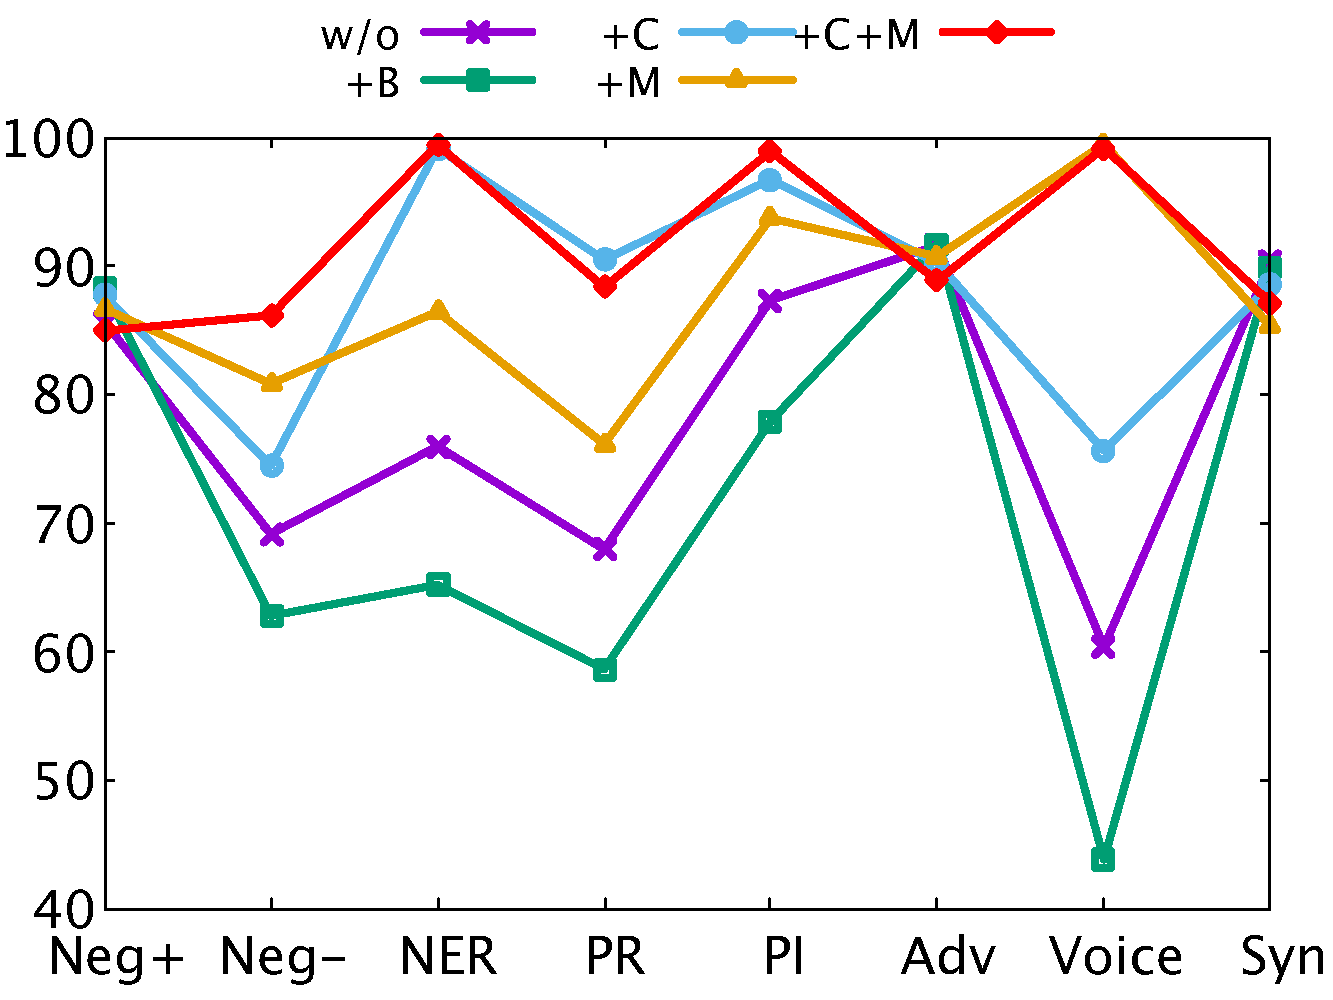
\includegraphics[width=0.6\columnwidth]{data/roc_roberta.pdf}
%   \caption{Detailed stress test with different aspects on ROC dataset. The x-axis indicates different stress test aspects and the y-axis indicates model accuracy in percentage.}
%   \label{fig:detailed}
% \end{figure}


%\begin{figure*}[!th]
%\centering
%\begin{subfigure}[b]{0.28\textwidth}
%\centering
%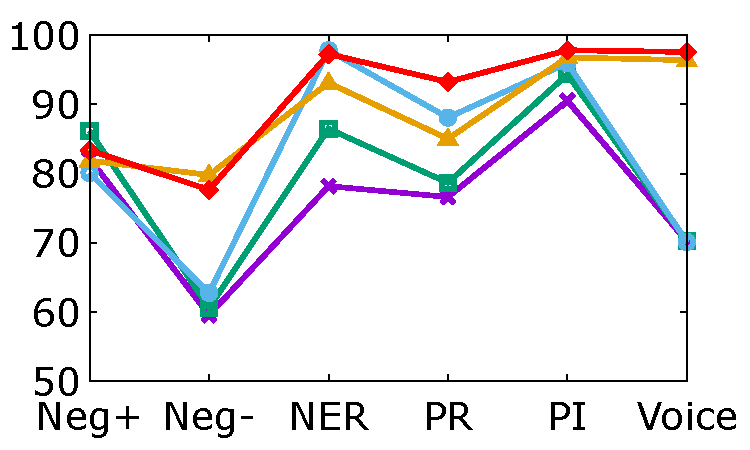
\includegraphics[width=\columnwidth]{data/roc_bert.pdf}
%\caption{BT (ROC)}
%\label{fig:roc_bert}
%\end{subfigure}
%\hfill
%\begin{subfigure}[b]{0.28\textwidth}
%\centering
%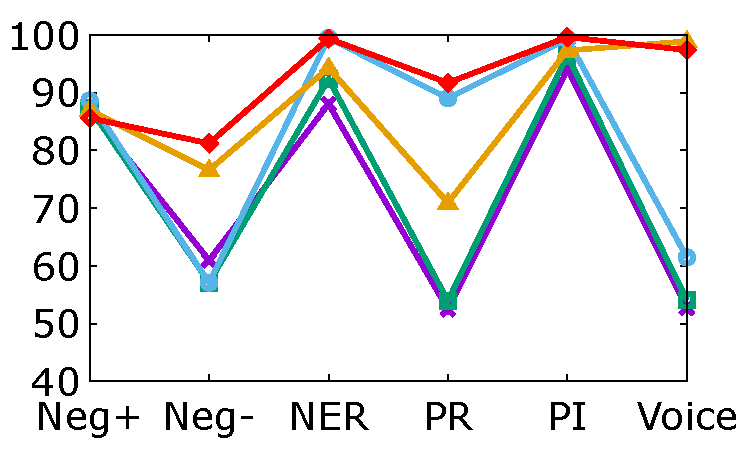
\includegraphics[width=\columnwidth]{data/roc_xlnet.pdf}
%\caption{XL (ROC)}
%\label{fig:roc_xlnet}
%\end{subfigure}
%\hfill
%\begin{subfigure}[b]{0.28\textwidth}
%\centering
%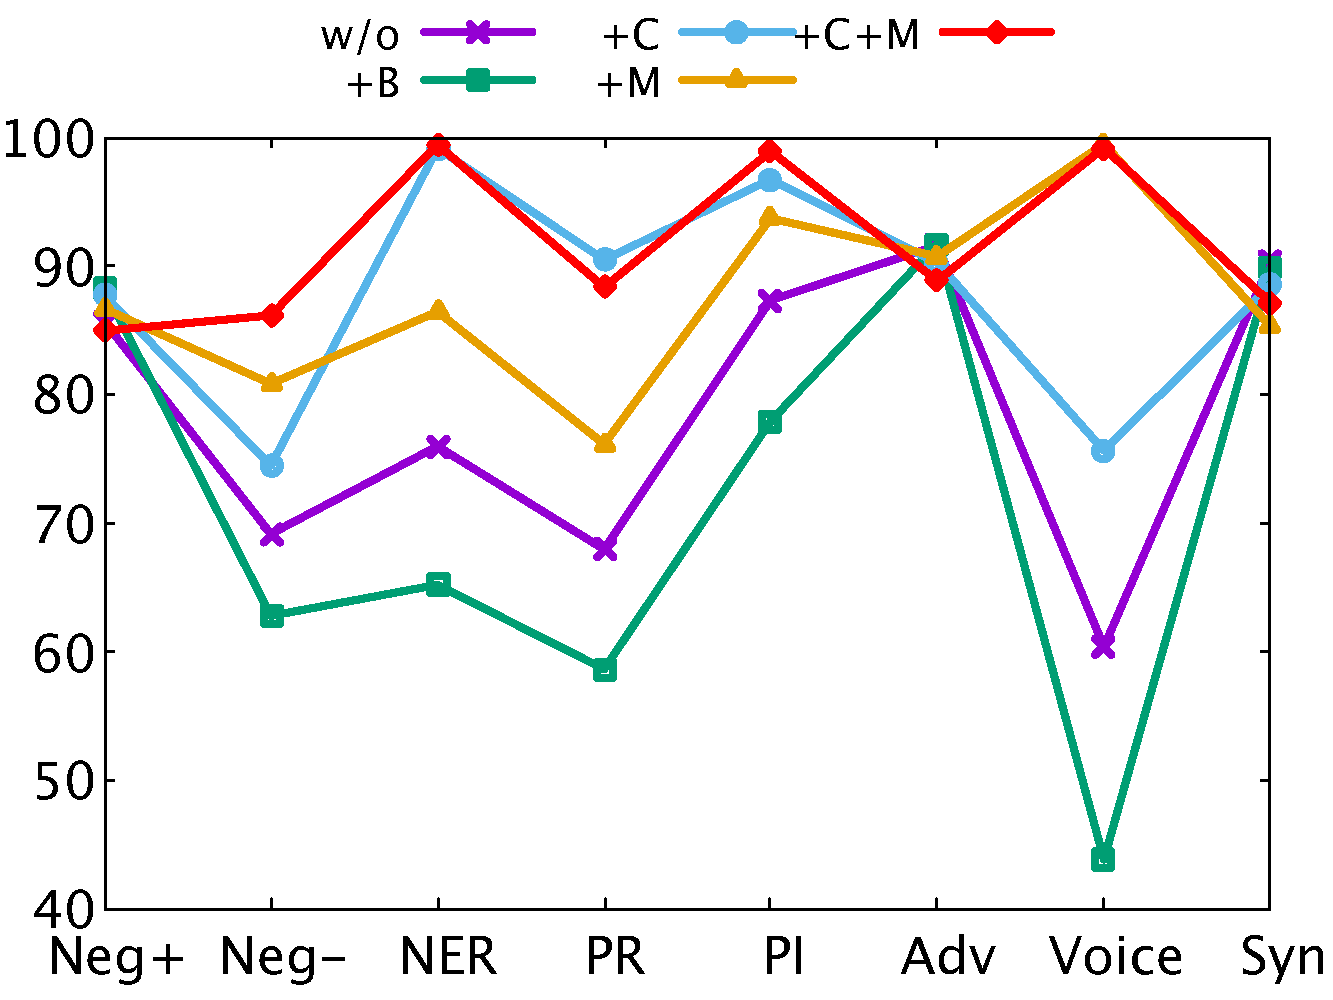
\includegraphics[width=\columnwidth]{data/roc_roberta.pdf}
%\caption{RB (ROC)}
%\label{fig:roc_roberta}
%\end{subfigure}
%\newpage
%\begin{subfigure}[b]{0.28\textwidth}
%\centering
%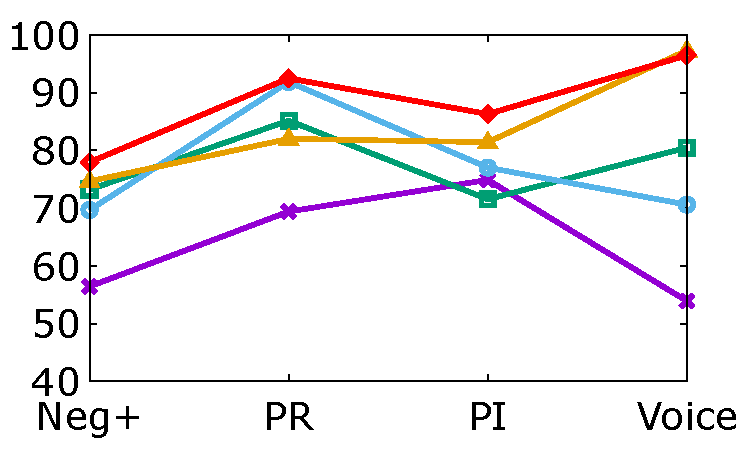
\includegraphics[width=\columnwidth]{data/copa_bert.pdf}
%\caption{BT (COPA)}
%\label{fig:copa_bert}
%\end{subfigure}
%\hfill
%\begin{subfigure}[b]{0.28\textwidth}
%\centering
%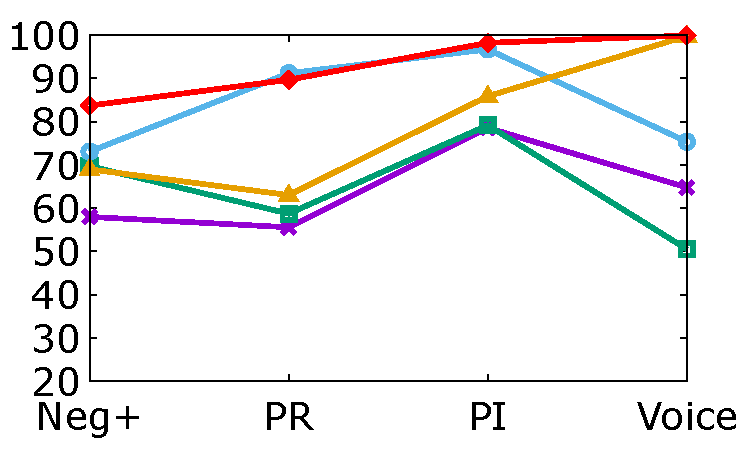
\includegraphics[width=\columnwidth]{data/copa_xlnet.pdf}
%\caption{XL (COPA)}
%\label{fig:copa_xlnet}
%\end{subfigure}
%\hfill
%\begin{subfigure}[b]{0.28\textwidth}
%\centering
%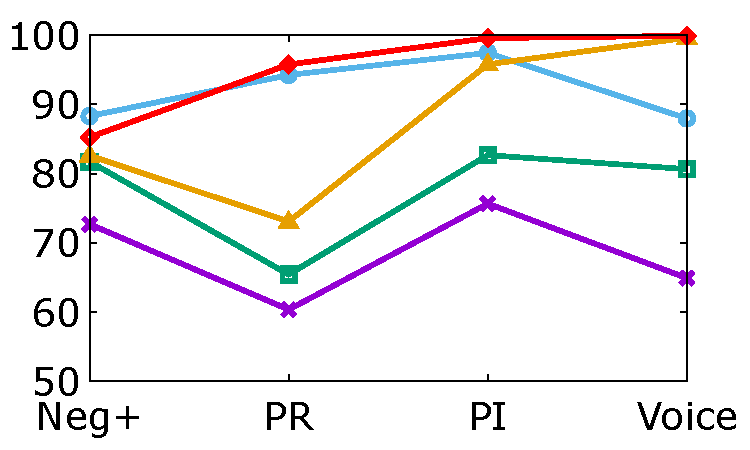
\includegraphics[width=\columnwidth]{data/copa_roberta.pdf}
%\caption{RB (COPA)}
%\label{fig:copa_roberta}
%\end{subfigure}
%\newpage
%\begin{subfigure}[b]{0.28\textwidth}
%\centering
%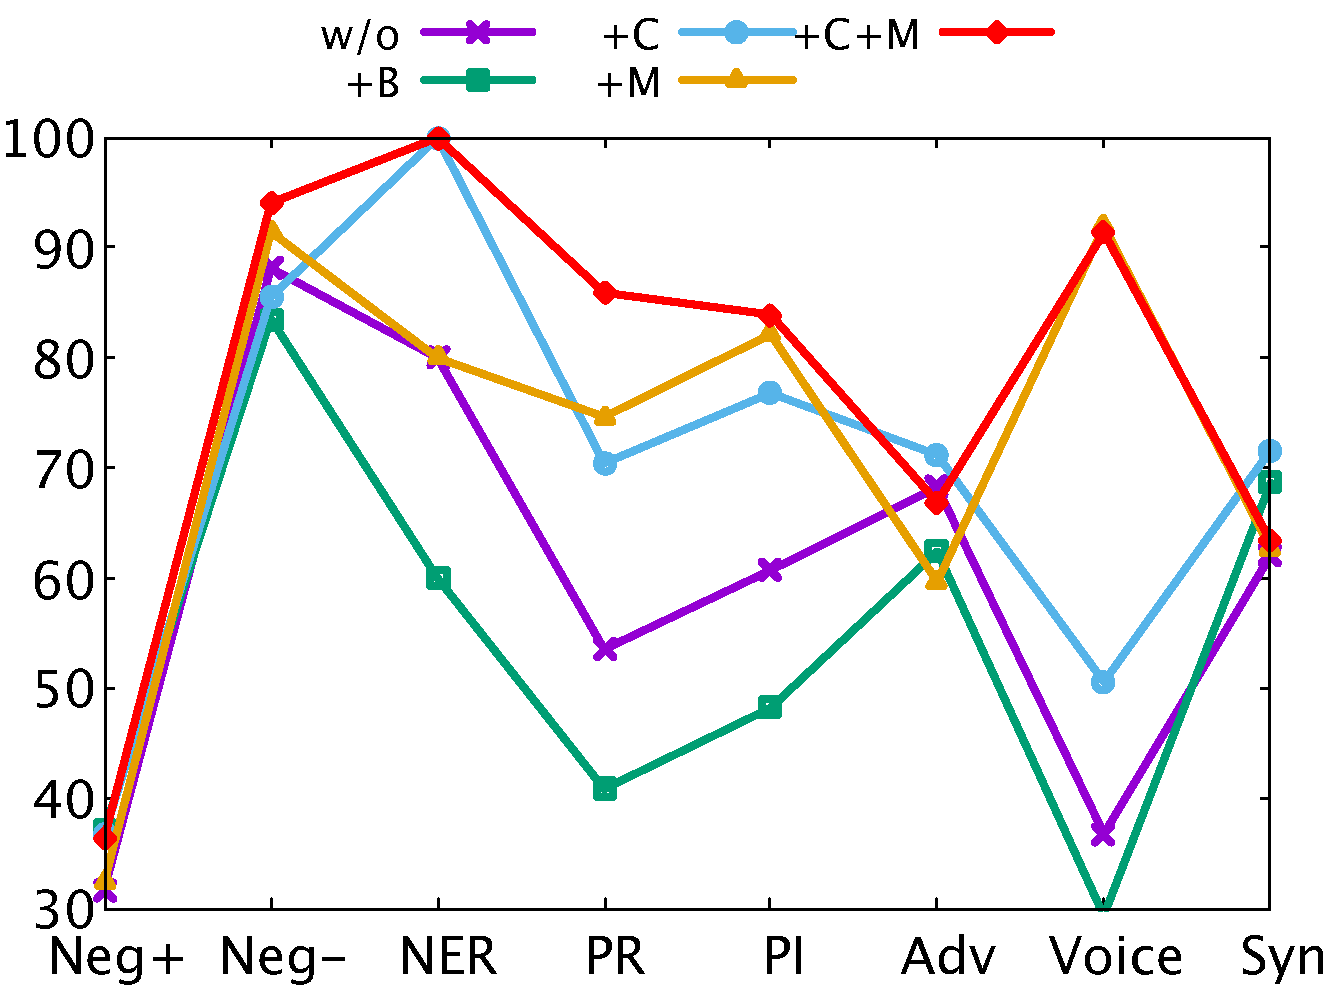
\includegraphics[width=\columnwidth]{data/arct_bert.pdf}
%\caption{BT (ARCT)}
%\label{fig:arct_bert}
%\end{subfigure}
%\hfill
%\begin{subfigure}[b]{0.28\textwidth}
%\centering
%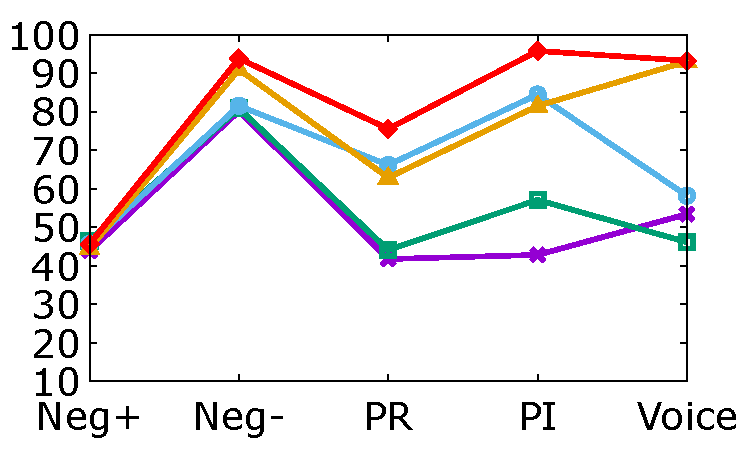
\includegraphics[width=\columnwidth]{data/arct_xlnet.pdf}
%\caption{XL (ARCT)}
%\label{fig:arct_xlnet}
%\end{subfigure}
%\hfill
%\begin{subfigure}[b]{0.28\textwidth}
%\centering
%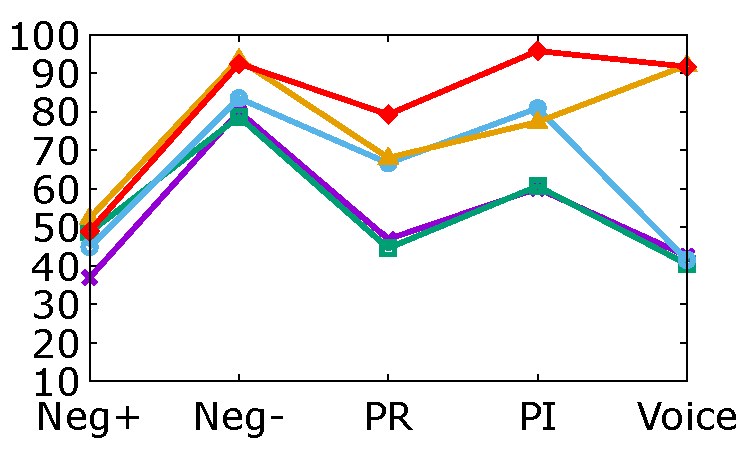
\includegraphics[width=\columnwidth]{data/arct_roberta.pdf}
%\caption{RB (ARCT)}
%\label{fig:arct_roberta}
%\end{subfigure}
%\newpage
%\begin{subfigure}[b]{0.28\textwidth}
%\centering
%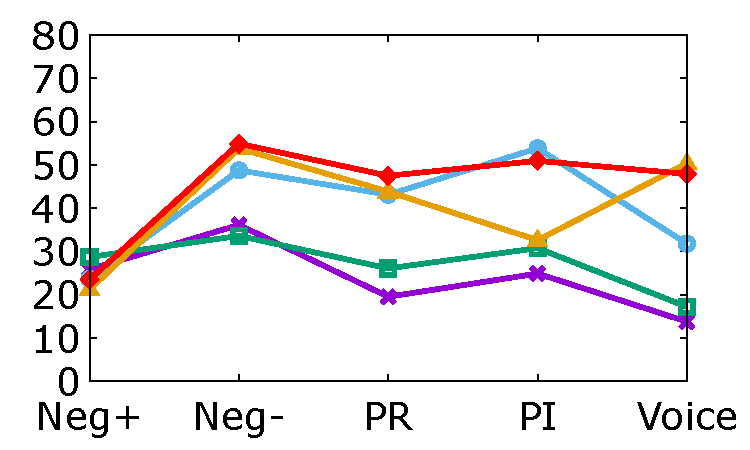
\includegraphics[width=\columnwidth]{data/reclor_bert.pdf}
%\caption{BT (RECLOR)}
%\label{fig:reclor_bert}
%\end{subfigure}
%\hfill
%\begin{subfigure}[b]{0.28\textwidth}
%\centering
%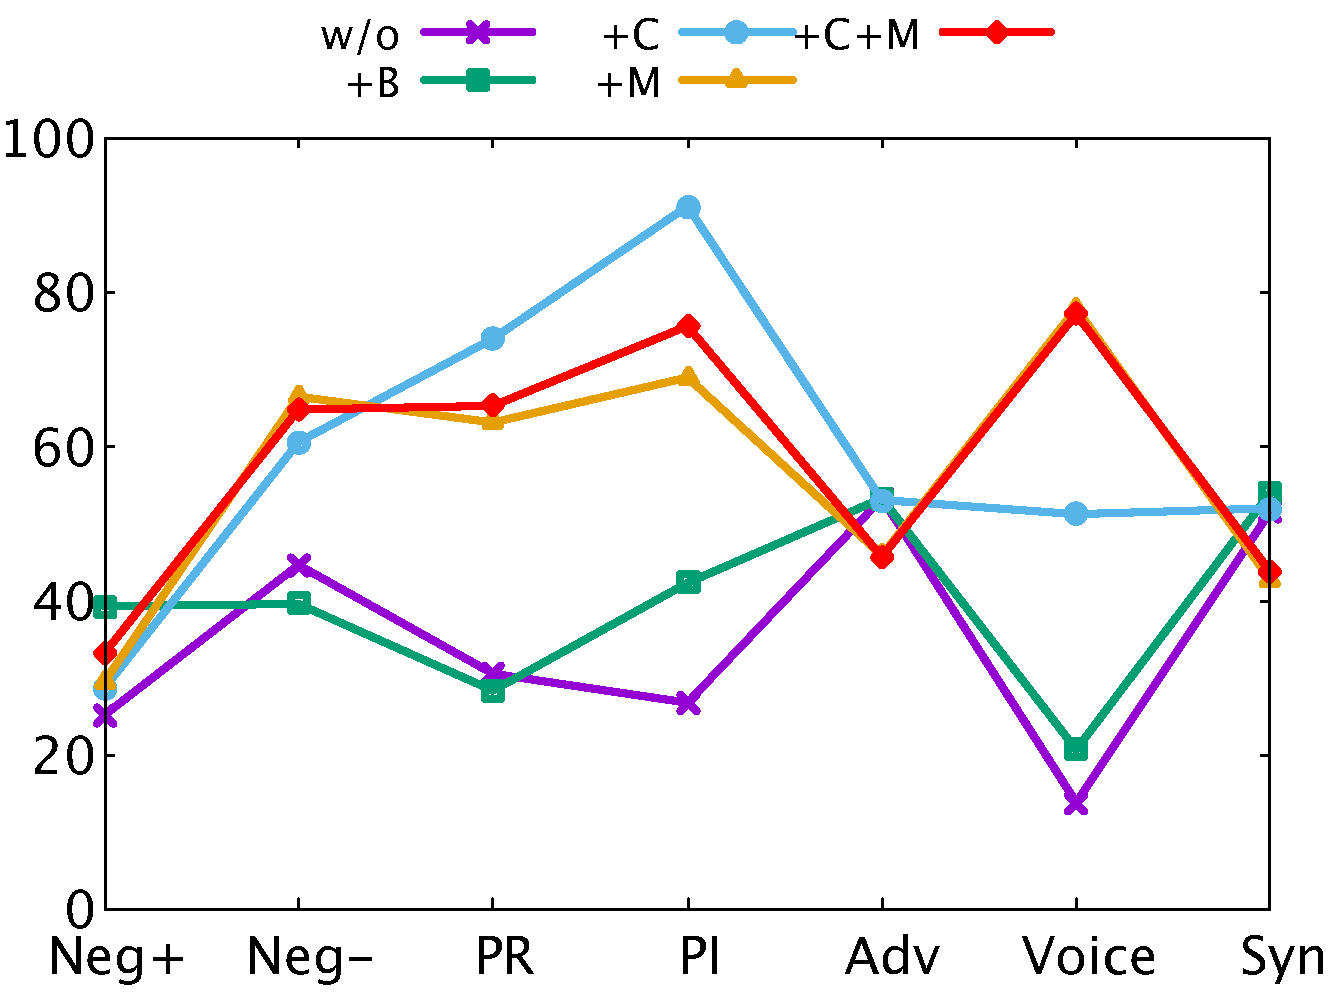
\includegraphics[width=\columnwidth]{data/reclor_xlnet.pdf}
%\caption{XL (RECLOR))}
%\label{fig:reclor_xlnet}
%\end{subfigure}
%\hfill
%\begin{subfigure}[b]{0.28\textwidth}
%\centering
%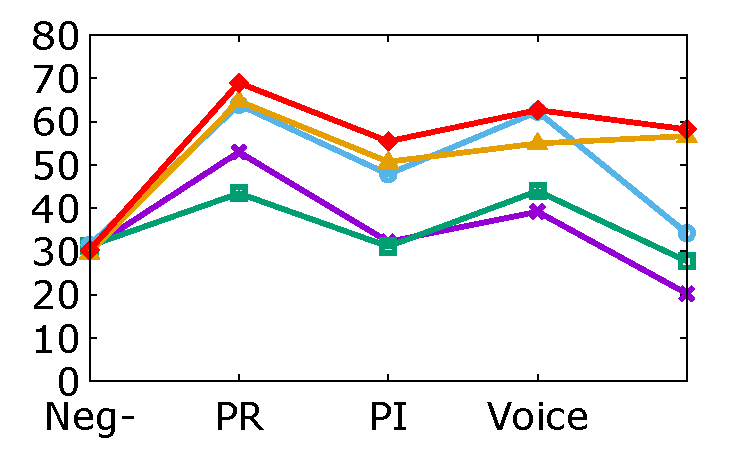
\includegraphics[width=\columnwidth]{data/reclor_roberta.pdf}
%\caption{RB (RECLOR)}
%\label{fig:arct_roberta}
%\end{subfigure}
%\newpage
%\begin{subfigure}[b]{1.0\textwidth}
%\centering
%
\includegraphics[width=0.4\columnwidth]{data/label.jpg}
%\label{fig:label}
%\end{subfigure}
%\caption{Fine-grained stress test with different aspects on 4 different tasks. 
%The x-axis in the figures indicates different stress test aspects and the y-axis indicates model accuracy in percentage.}
%%\KZ{Caption is wrong! most graphs are fine. 
%%But ReCLOR (RB) is a bit strange. 
%%Why is BT line exactly the same as the BT+C? And why is BT+B so bad?}}
%\label{fig:detail}
%\end{figure*}
%%
%
\begin{figure*}[!th]
\centering
\begin{subfigure}[b]{0.24\textwidth}
\centering
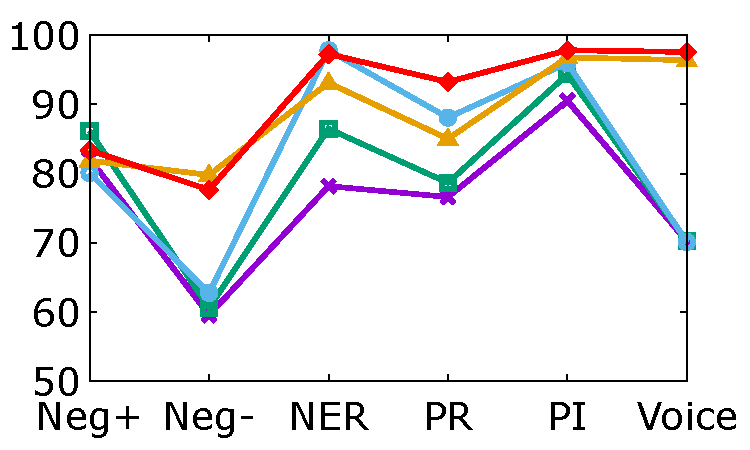
\includegraphics[width=\columnwidth]{data/roc_bert.pdf}
\caption{BT (ROC)}
\label{fig:roc_bert}
\end{subfigure}
\hfill
\begin{subfigure}[b]{0.24\textwidth}
\centering
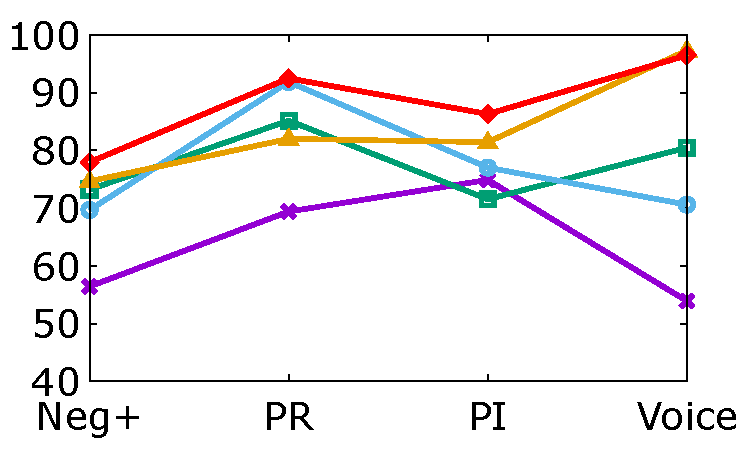
\includegraphics[width=\columnwidth]{data/copa_bert.pdf}
\caption{BT (COPA)}
\label{fig:copa_bert}
\end{subfigure}
\hfill
\begin{subfigure}[b]{0.24\textwidth}
\centering
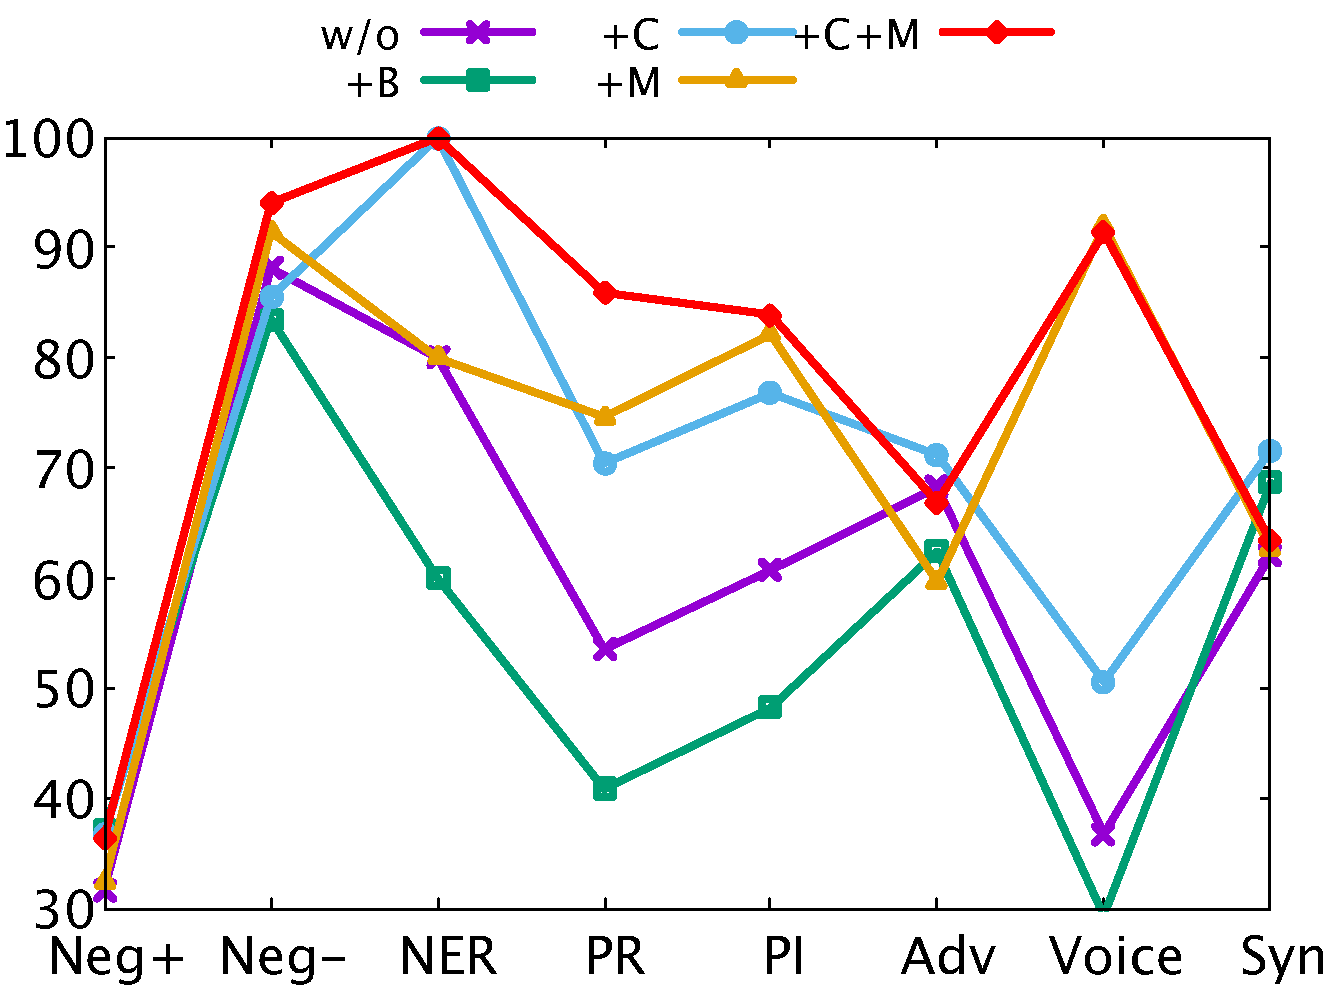
\includegraphics[width=\columnwidth]{data/arct_bert.pdf}
\caption{BT (ARCT)}
\label{fig:arct_bert}
\end{subfigure}
\hfill
\begin{subfigure}[b]{0.24\textwidth}
\centering
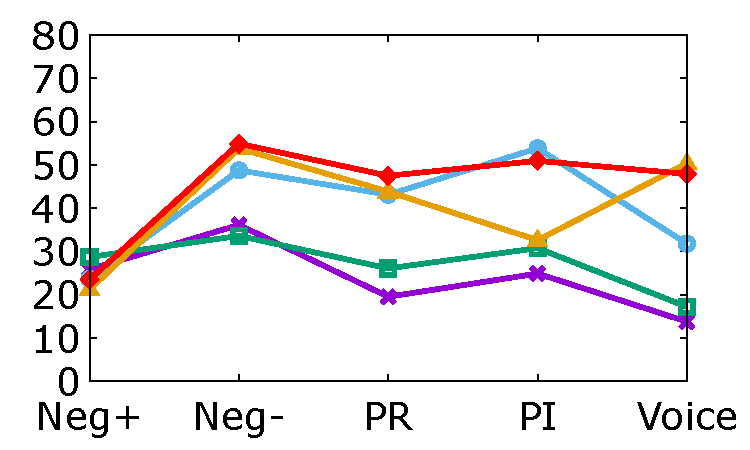
\includegraphics[width=\columnwidth]{data/reclor_bert.pdf}
\caption{BT (RECLOR)}
\label{fig:reclor_bert}
\end{subfigure}
\newpage
\begin{subfigure}[b]{0.24\textwidth}
\centering
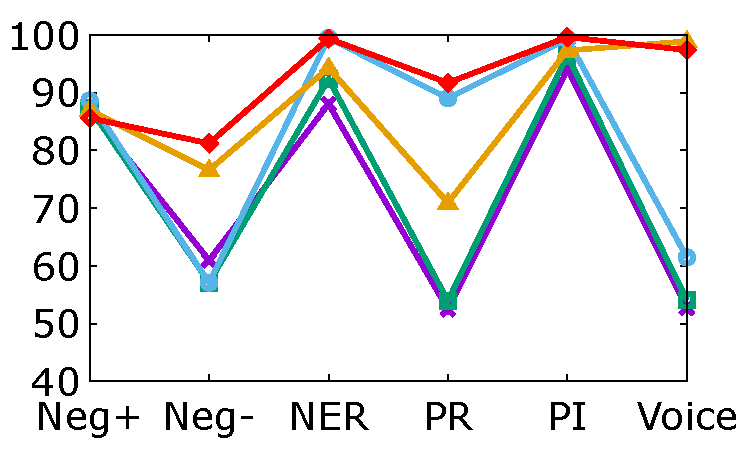
\includegraphics[width=\columnwidth]{data/roc_xlnet.pdf}
\caption{XL (ROC)}
\label{fig:roc_xlnet}
\end{subfigure}
\hfill
\begin{subfigure}[b]{0.24\textwidth}
\centering
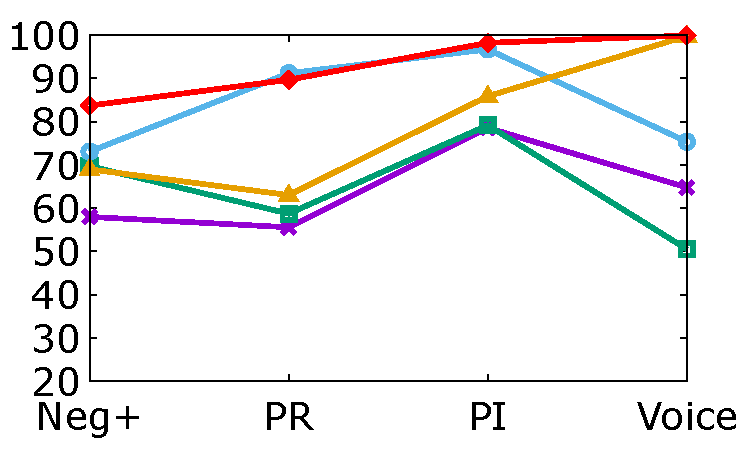
\includegraphics[width=\columnwidth]{data/copa_xlnet.pdf}
\caption{XL (COPA)}
\label{fig:copa_xlnet}
\end{subfigure}
\hfill
\begin{subfigure}[b]{0.24\textwidth}
\centering
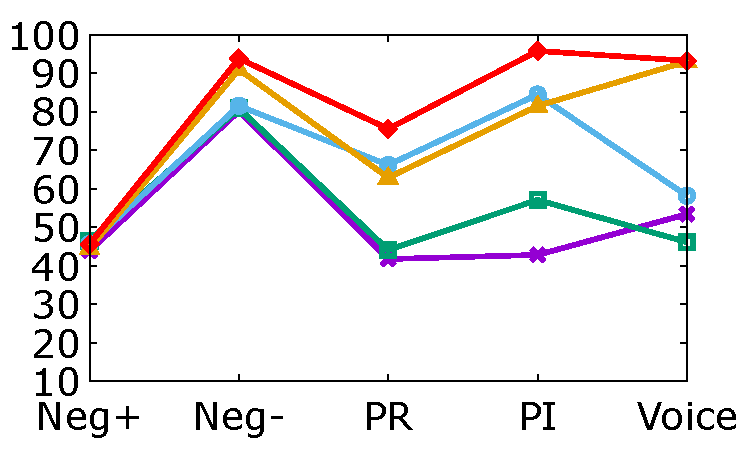
\includegraphics[width=\columnwidth]{data/arct_xlnet.pdf}
\caption{XL (ARCT)}
\label{fig:arct_xlnet}
\end{subfigure}
\hfill
\begin{subfigure}[b]{0.24\textwidth}
\centering
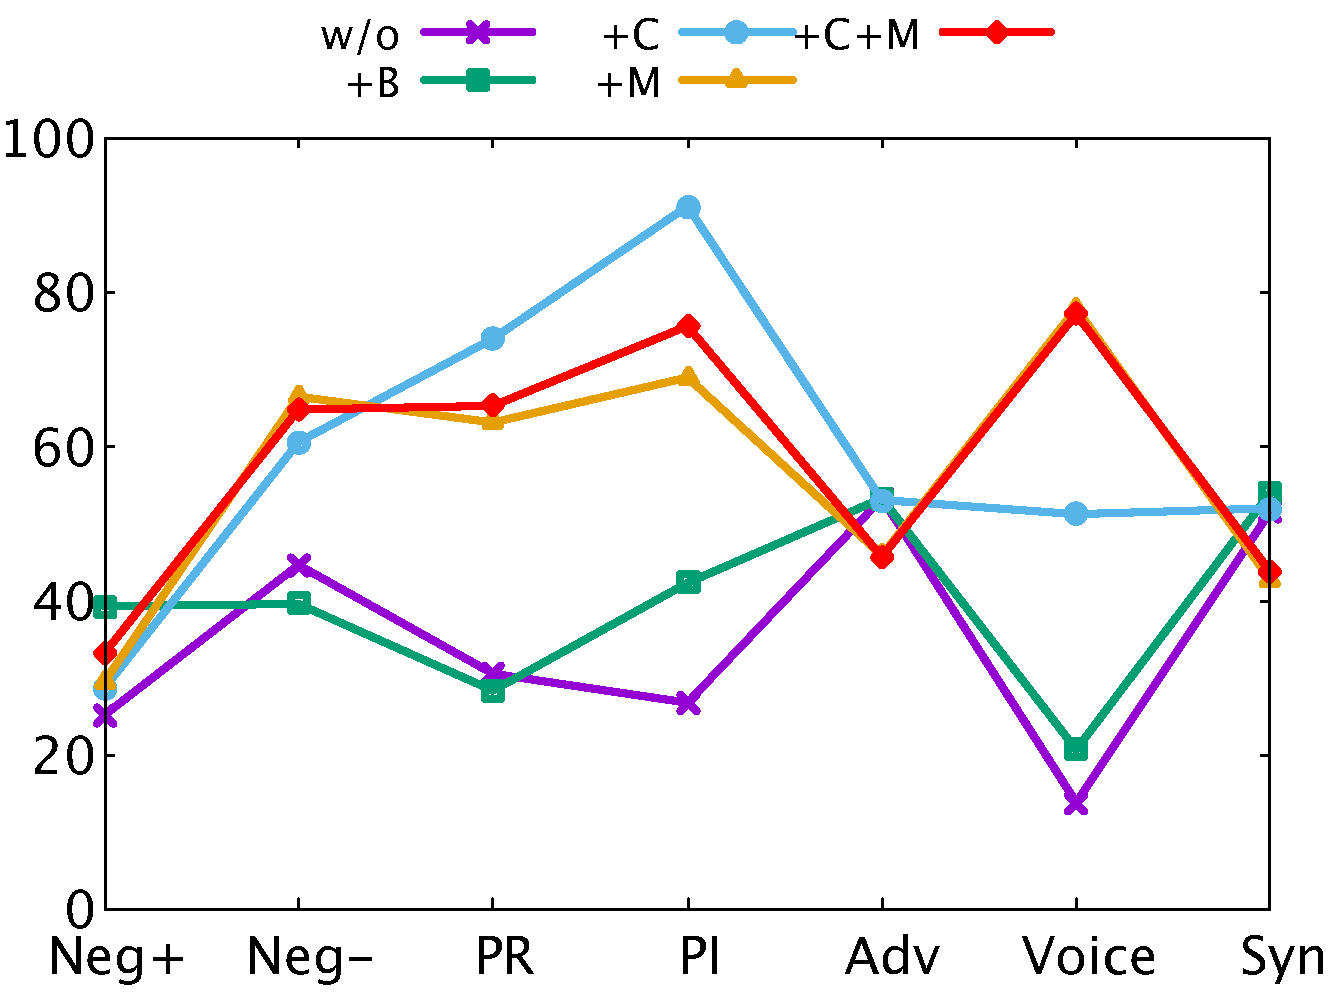
\includegraphics[width=\columnwidth]{data/reclor_xlnet.pdf}
\caption{XL (RECLOR))}
\label{fig:reclor_xlnet}
\end{subfigure}
\newpage
\begin{subfigure}[b]{0.24\textwidth}
\centering
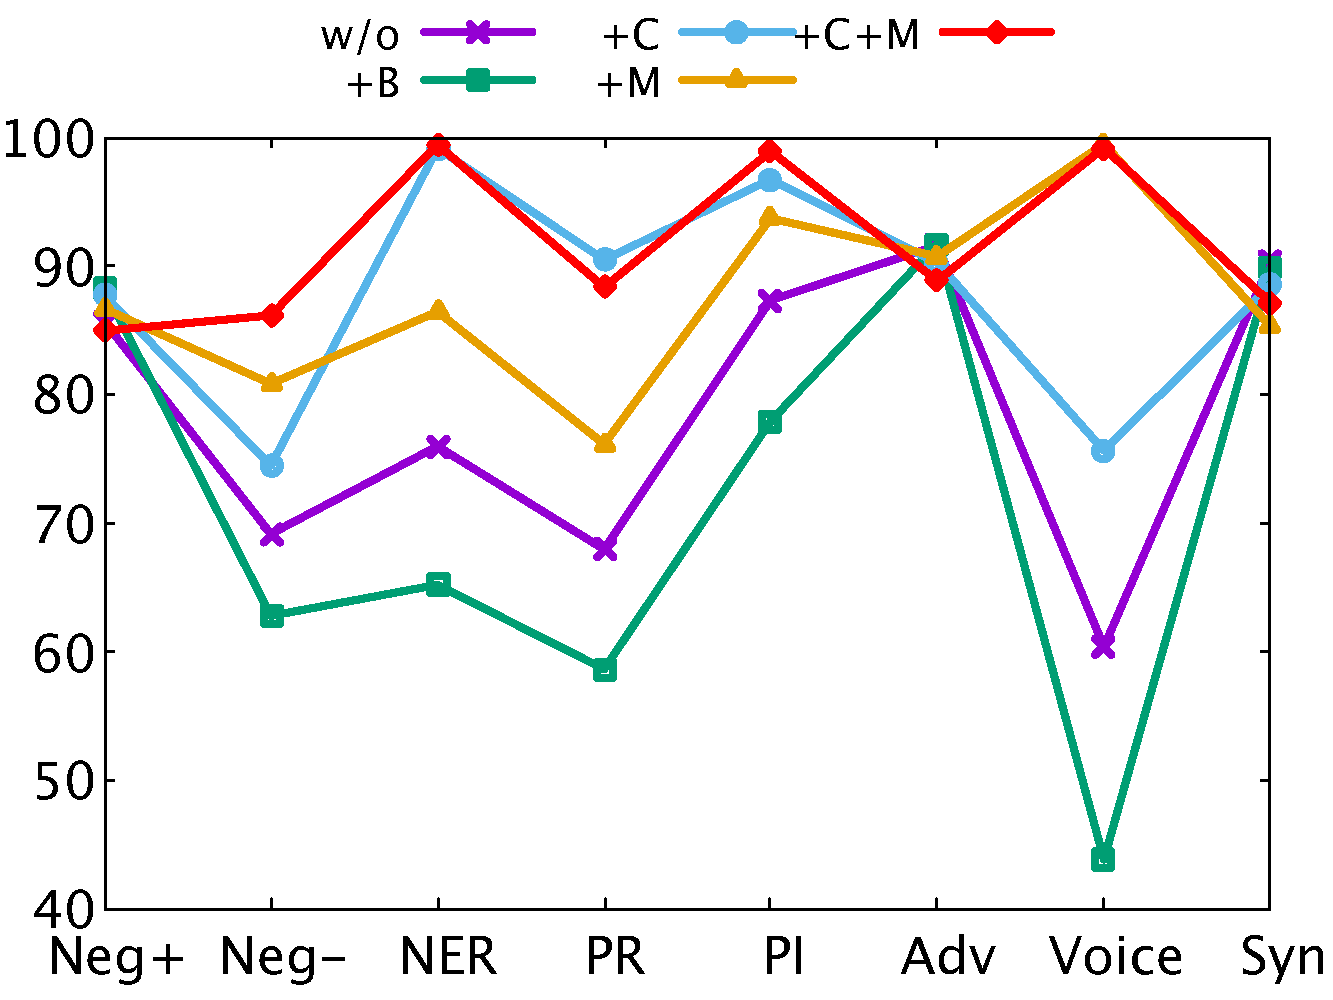
\includegraphics[width=\columnwidth]{data/roc_roberta.pdf}
\caption{RB (ROC)}
\label{fig:roc_roberta}
\end{subfigure}
\hfill
\begin{subfigure}[b]{0.24\textwidth}
\centering
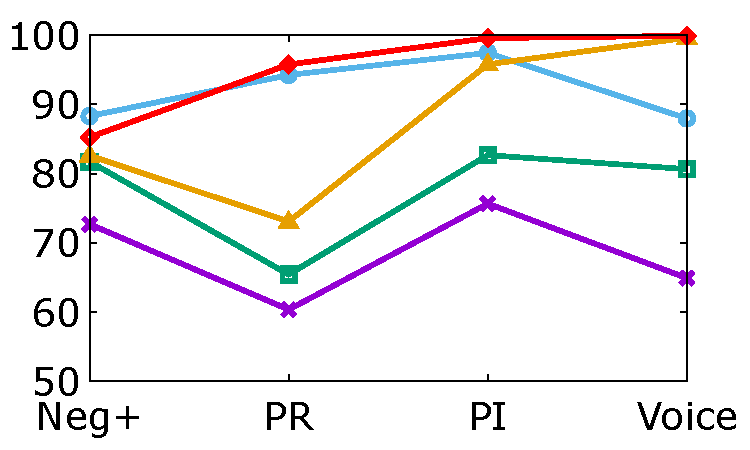
\includegraphics[width=\columnwidth]{data/copa_roberta.pdf}
\caption{RB (COPA)}
\label{fig:copa_roberta}
\end{subfigure}
\hfill
\begin{subfigure}[b]{0.24\textwidth}
\centering
\includegraphics[width=\columnwidth]{data/arct_roberta.pdf}
\caption{RB (ARCT)}
\label{fig:arct_roberta}
\end{subfigure}
\hfill
\begin{subfigure}[b]{0.24\textwidth}
\centering
\includegraphics[width=\columnwidth]{data/reclor_roberta.pdf}
\caption{RB (RECLOR)}
\label{fig:arct_roberta}
\end{subfigure}
\newpage
\begin{subfigure}[b]{1.0\textwidth}
\centering
\includegraphics[width=0.4\columnwidth]{data/label.jpg}
\label{fig:label}
\end{subfigure}
\caption{Fine-grained stress test with different aspects on 4 different tasks. 
The x-axis in the figures indicates different stress test aspects and the y-axis indicates model accuracy in percentage.}
%\KZ{Caption is wrong! most graphs are fine. 
%But ReCLOR (RB) is a bit strange. 
%Why is BT line exactly the same as the BT+C? And why is BT+B so bad?}}
\label{fig:detail}
\end{figure*}
%
\subsubsection{Fine-grained results}
\label{sec:fine-grained}
We proceed to break down the results in \tabref{tab:stressresults} into accuracies on stress tests
created by different operators. 
%We show the detailed results in~\figref{fig:detail} 
%Concretely, six different aspects of stress test data are 
%utilized for testing.
COPA and RECLOR datasets do not show all six operators
because some of the operators generate too little data
for them, as shown in \tabref{tab:cases}. 
%The x-axis in the figures indicates different stress test aspects 
%and the y-axis indicates model accuracy in percentage.
%We apply the proposed two operators \textit{crossover} and \textit{mutation} to BERT, XLNet and RoBERTa 
%models and compare it with back-translation.
%and test on various stress test cases with different aspects. 
The corresponding results are presented in~\figref{fig:detail}. 
We observe that the vanilla model in purple and back-translation in green show
worse results across different aspects than other lines. 
The models trained with data augmented by \textit{crossover} and \textit{mutation} 
(the red lines) are generally more robust than others.
%\KZ{It is consistent with our overall results in~\tabref{tab:results}.} 
Please refer to Appendix A. 
%\footnote{There are some dashes in the table because the } 
for complete results. 
%\KZ{You need to explain why there are some dashes in the table in appendix.}

%We also observe that the 
%accuracy performance points for ``Syn'' and ``Adv'' are concentrated 
%but scattered on other operator aspects. 
Since every type of stress tests 
%(except ``Syn'' and ``Adv) 
can evaluate if a model is robust, particularly if it considers the 
premise by giving it two very similar choices, 
the above results on the stress tests of all types show that our two methods do 
%improves the model robustness, and may even encourage the models to look toward the
reduce short-circuits, and may even encourage the models to look toward the
premises.
We will provide additional pieces of evidence to confirm this in the next two subsections.

%\KZ{The weakness can be on the same table as the improvements
%to save space.}
%\KZ{Check the following analysis to make sure it's consistent with the tables.}

%Compared with 
%base models without data augmentation, we find that 
%all four data augmentation methods moderately improve
%the models when tested on the original test set. 
%In ROC, accuracy of BERT and RoBERTa trained with crossover augmented data 
%exceeds base models and ranks top. Crossover method also works on COPA. 
%Even though back-translation obtains higher score mostly on ARCT and RECLOR,
%crossover, mutation and crossover+mutation barely fall below the base model. 
%
%Augmentation fares much better in the ``Stress'' columns, though
%different methods show varying degree of success.
%Compared with the model without data augmentation, 
%the performance of models with crossover 
%has always been greatly improved (i.e., by 21.44\% for BERT on COPA).
%It indicates that reducing the short circuits 
%is a good way to improve the robustness of a model.
%The performance of new models with crossover has 
%great improvement for all models on different dataset 
%compared with the model without data augmentation, like 21.44% for BERT on COPA. 
%Mutation alone can also help with robustness on stress test better than crossover.
%This result suggests that mutation is a good method 
%for enhancing the robustness of models. 
%Though, mutation may be not a 
%good method to decrease the short circuits (\secref{sec:fix-sc}). 
%Overall, crossover+mutation 
%can mostly get the best performance on the stress test except for 
%training on RECLOR with RoBERTa. 
%to This result indicates that this kind of data can prevent models from being confused 
%by simple perturbations thus improving the robustness of models. 
%Besides, we can also find that back-translation doesn't improve the models' robustness much.
%Crossover alone can also help with robustness on stress test but 
%no better than mutation and crossover+mutation.  

%some of Table 5's AW scores being 
%some of Table 5's AW scores being 
%lower than AW for model w/o augmentation (e.g., 45.13 in (b)), 
%then the reason is AW is only a proxy test
%that catches majority of short circuit cases in our opinion, 
%but it's not perfect, as we pointed out in A2 of R1. 
%If you are referring to some accuracies in the Original columns 
%being lower than models w/o augmentation in Table 5 (e.g., 72.6 in (b)), 
%the reason is some models w/o augmentation might have 
%"cheated" to get high accuracy. Augmenting (C or M) corrects the
%biases in these models and may reduce the accuracy on the original test set.
%Nevertheless, all models after augmentation do better on the stress tests.

%have least short circuits based on BERT and XLNet. 
%Crossover+mutation based on RoBERTa takes less short circuits than others. 
%In the CO and AW columns, the result are consistent on ROC. 

%\subsection{White-box Attention Weights~(AW)}
%\KZ{Here we first talk about human testing by visualizastion,
%then talk about how to automatic it thru code.}

%show human annotation results of bert, roberta, xlnet.
%For exploiting whether attention-based models are suffered from short circuits, 
%we propose to 
%use the AW method which we have described in~\secref{}.
%It is noted that t\_1 is greater than t\_2. 
%Here t\_1 and t\_2 are tuned to 0.14 and 0.13 separately.

\subsection{Choice-only Test}
\label{sec:choice-only}

%In this section, we use choice-only test for different models on four tasks. 
%We have shown the effectiveness of \textit{crossover} and \textit{mutation} on in robustness test. 
The end-to-end test has shown the success of our data augmentation 
methods. To further explore the reason behind the performance gain, 
we also use choice-only test here.

%somewhat confirm the reason for model improvement with data augmentation 
%strategies. Moreover, this test is used to further explore 
%whether our strategies can encourage models pay more attention to premise.
In choice-only test, we only feed choices into a model without a premise which is replaced 
by an empty string. This way, 
models cannot utilize the relationship between premise and choices. 
%what we can know whether a model can 
%solve cases easily without awaring premise by test accuracy. 
Normally, we would expect the model to make arbitrary choices.
However, if a model can easily ``guess'' the ``right'' choice which 
normally requires the relationship between premise and choices,  
one possibility is that this model cheats on evaluation procedure and 
may be fragile. Thus, the higher score may indicate more use of short-circuits.

In~\figref{fig:choice-only}, we observe that in choice-only tests,
the accuracy of models augmented with \textit{crossover} and \textit{mutation} 
(red line) drops the most. 
Sometimes the performances are similar to random selection, e.g., 
RB+C+M on ARCT (56.38\%), which indicates that models 
are no longer cheating. 
In other words, models augmented by crossover and mutation 
are more likely to consider the premises. 
The results on the choice-only tests provide another perspective for us
to re-assure that models augmented with crossover and mutation can reduce
short circuits and thus model fragility.

%\KZ{Rephrase: 
%However, another possibility reason for lower choice-only test accuracy 
%that is also not ruled out is that 
%even if the model can tell the result with only choices, 
%it still chooses to look at the premise context. 
%Although high scores do not necessarily imply models 
%are not looking forward, low scores necessarily mean that models cannot 
%conclude that solely relying on choices.} 

%\begin{table}[th]
%\centering
%\scriptsize
%\begin{tabular}{c|rrrr}
%\toprule
%\textbf{Model} & \textbf{ROC} & \textbf{COPA} & \textbf{ARCT} & \textbf{RECLOR} \\ \midrule
%%BT  &98.76 &89.68&\textbf{99.65}&82.46    \\ \hline
%%BT+B  &99.26 &96.79   &99.34  &86.01  \\ \hline
%%BT+C  &\textbf{99.69} &\textbf{98.35}&98.37   &80 \\ \hline
%%BT+M  &99.26 & 95.17 &98.67 &82.48    \\ \hline
%%BT+C+M  &98.82 &96.96 &98.00 &\textbf{96.79}  \\ \midrule
%%XL  &28.08 &93.16 & 85.67 & 79.64 \\ \hline
%%XL+B  &19.27  &91.46 &95.73 & 81.40   \\ \hline
%%XL+C  &\textbf{64.58} &45.13  &55.59  &\textbf{87.87} \\ \hline
%%XL+M  &62.77  &96.85 & \textbf{95.74}& 72.76  \\ \hline
%%XL+C+M  &60.25 & \textbf{98.51}&86.26 &   48.71\\ \midrule
%%RB  &77.41 & 80.89 & 99.14& 85.88 \\ \hline
%%RB+B  &   58.15 &\textbf{96.36}   & 97.78& 15.69  \\ \hline
%%RB+C  &   82.71& 89.62&79.19& 89.68\\ \hline
%%RB+M  &71.73& 62.26& \textbf{100.00}&\textbf{100.00}  \\ \hline
%%RB+C+M  &\textbf{93.31} &61.89    &71.47 & 89.26\\ 
%%
%BT (w/o)&54.62&51.4&61.94&42.8 \\ \hline
%BT+B&58.26&50.8&64.41&39.2  \\ \hline
%BT+C&51.2&48.2&55.63&30.8  \\ \hline
%BT+M&51.79&48.8&55.18&38   \\ \hline
%BT+C+M&43.56&49.4&52.03&33.8  \\ \midrule
%XL (w/o)&71.14&57&65.99&42.2 \\ \hline
%XL+B&73.17&60&66.89&41.4  \\ \hline
%XL+C&65.63&55&55.86&34.2  \\ \hline
%XL+M&71.94&57.8&66.22&42  \\ \hline
%XL+C+M&66.22&58.4&62.84&35  \\ \midrule
%RB (w/o)&73.97&59.4&67.79&30.2 \\ \hline
%RB+B&74.77&61.4&69.37&42.2  \\ \hline
%RB+C&73.06&58.4&68.47&34.6  \\ \hline
%RB+M&70.34&56&61.49&40      \\ \hline
%RB+C+M&71.3&54.8&67.79&32.2  \\ 
%\bottomrule
%\end{tabular}
%\caption{Choice-only test for transformer-based models on 4 datasets. All numbers are percentages (\%)}
%%\KZ{I assume this is the ending-only test? But isn't scriptsizeer the better
%%for ending-only tests?}}
%\label{tab:only-test}
%\end{table}
%
\begin{figure}[th]
    \centering
    \includegraphics[width=0.7\columnwidth]{data/choice-only.pdf}
    \caption{Choice-only test: Accuracies of different data augmentation methods with 3 models on 4 tasks. 
    The detailed numbers are in Appendix B.}
    \label{fig:choice-only}
\end{figure}

However, one may argue that even if a model can 
choose or ``guess'' correctly given only the choices but no premise, 
it may still have the ability to look at the premise if it's given one,
like in the end-to-end test.
Therefore, next we conduct an additional case study to show that short-circuit
does take place and our augmentation methods alleviate it.

\subsection{Case Study}
\label{sec:case}

%\begin{figure}[th!]
%\centering
%\begin{subfigure}[b]{0.21\textwidth}
%\centering
%
%\framebox{\includegraphics[width=\columnwidth]{figure/case_original.eps}}
%\caption{RB(w/o)}
%\label{fig:case_original}
%\end{subfigure}
%\hfill
%\begin{subfigure}[b]{0.21\textwidth}
%\centering
%\framebox{\includegraphics[width=\columnwidth]{figure/case_b.eps}}
%\caption{RB+B}
%\label{fig:case_b}
%\end{subfigure}
%\hfill
%\newpage
%\begin{subfigure}[b]{0.21\textwidth}
%\centering
%\framebox{\includegraphics[width=\columnwidth]{figure/case_c.eps}}
%\caption{RB+C}
%\label{fig:case_c}
%\end{subfigure}
%\hfill
%\begin{subfigure}[b]{0.21\textwidth}
%\centering
%\framebox{\includegraphics[width=\columnwidth]{figure/case_cm.eps}}
%\caption{RB+C+M}
%\label{fig:case_cm}
%\end{subfigure}
%\caption{Attention map on a COPA example for models.}
%%\KZ{Caption is wrong! most graphs are fine. 
%%But ReCLOR (RB) is a bit strange. 
%%Why is BT line exactly the same as the BT+C? And why is BT+B so bad?}}
%\label{fig:case}
%\end{figure}
%

%In \figref{fig:case}, 
%%illustration. There is no positive attention value in front of the 
%%fourth sentence, so we intercept it from where it is worth. 
%RoBERTa trained on the original training set fails to pick up the 
%relation between ``pushed'' and ``opened''. 
%%right choice likely due to there being virtually no attention 
%%connection between words in the choice and words in the premise. 
%After training with \textit{crossover} data augmentation, 
%the model learns to build contextual reasoning  
%by attending to relevant concepts in the premise. 
%%i.e., ``show'' in this example. The rationale behind 
%%such a change of attention pattern is that, 
%%in a MCQ created by crossover operation, 
%%the model needs to combine information 
%%in the premise to effectively 
%%distinguish the true ``right'' choice from the wrong one, 
%%which is also a right choice in another MCQ. 
%to have not enhanced such abilities. We provide additional cases in Appendix C.

%\begin{figure}[th]
%\centering
%{\setlength{\fboxsep}{0pt}
%5\framebox{%
%\includegraphics[width=0.47\columnwidth]{figure/o_un.eps}
%}
%\hfill
%\framebox{%
%\includegraphics[width=0.47\columnwidth]{figure/cross_un.eps}
%}
%}
%\caption{Attention maps showing that RoBERTa short-circuits on a ROC
%question (left) and no longer short-circuits after data augmentation (right). \KZ{I suggest we show a few more cases here to be more convincing. Show the before and after. Before there's no attention to the
%premise, after there is.}}
%\label{fig:case_study}
%\end{figure}

%\begin{example}\label{ex:roc}
%An MCQ from ROC:\\ \\
%\noindent
%\textbf{Premise:} Sarah was home alone. She wanted to stay busy. She turned on the TV. 
%She found a reality show to watch.  \\
%\textbf{Choice 1:} Sarah then happily watched the show.  \checksymbol  \\
%\textbf{Choice 2:} Sarah could not find anything to watch. \crosssymbol
%\end{example}

Our case study is a series of white-box tests that demonstrate
the change in attention patterns.

We take an example from ROC which is shown in~\tabref{table:dataset}.
We explore BERT-based models by 
analyzing their attention maps on this case in~\figref{fig:roc_bert}.  
In this example, the word ``show'' in the premise is strongly
related to the token ``reality show'' in the right choice from human knowledge. 
%The relationship between these two words is the key to answering this question. 
%We explore different models with the augmentation method with attention map 
%to visualize if these two words have a relationship or not.
The attention map is visualized via an off-the-shelf tool~\cite{vig-2019-multiscale}.


There is no positive attention value in front of the fourth sentence, 
so we intercept it from where it is worth. 
BERT trained on the original training set fails 
to pick up the right choice likely due to there being 
virtually no attention connection between words in 
the choice and words in the premise.
After training with \textit{crossover} data augmentation, 
the model learns  
to pay attention to the premise and the relationship 
between premise and choices. 
i.e., ``show'' in this example. 
Similar trends also exist for the \textit{mutation} operation in \figref{fig:roc_m} 
and the combination of \textit{crossover} 
and \textit{mutation} operation in~\figref{fig:roc_cm}. 
The rationale behind 
such a change of attention pattern is that, 
in an MCQ created by \textit{crossover} operation (\figref{fig:roc_c}), \textit{mutation}(\figref{fig:roc_m}), 
and the combination of them (\figref{fig:roc_cm}), 
the model needs to combine the information 
in the premise to effectively 
distinguish the true ``right'' choice from the wrong one. 
However, the light and sparse attention color blocks on the attention map for back-translation 
in \figref{fig:roc_b} indicate back-translation 
can not help BERT connect the choice and premise very well in this question.
These observations empirically demonstrate the effectiveness of our methods 
in encouraging the model to pay attention to the premise to reduce 
short circuits. We provide additional cases in Appendix C. 

%\begin{figure}[th!]
%\centering
%\begin{subfigure}[b]{0.35\textwidth}
%\centering
%\framebox{\includegraphics[width=\columnwidth]{figure/roc_b.eps}}
%\caption{BT+B}
%\label{fig:roc_b}
%\end{subfigure}
%\hfill
%\begin{subfigure}[b]{0.35\textwidth}
%\centering
%\framebox{\includegraphics[width=\columnwidth]{figure/roc_c.eps}}
%\caption{BT+C}
%\label{fig:roc_c}
%\end{subfigure}
%%\hfill
%\newpage
%\begin{subfigure}[b]{0.35\textwidth}
%\centering
%\framebox{\includegraphics[width=\columnwidth]{figure/roc_m.eps}}
%\caption{BT+M}
%\label{fig:roc_m}
%\end{subfigure}
%\hfill
%\begin{subfigure}[b]{0.35\textwidth}
%\centering
%\framebox{\includegraphics[width=\columnwidth]{figure/roc_cm.eps}}
%\caption{BT+C+M}
%\label{fig:roc_cm}
%\end{subfigure}
%\caption{Attention map on a ROC example for BERT-based models.}
%%\KZ{Caption is wrong! most graphs are fine. 
%%But ReCLOR (RB) is a bit strange. 
%%Why is BT line exactly the same as the BT+C? And why is BT+B so bad?}}
%\label{fig:roc_bert}
%\end{figure}
%
\begin{figure}[h!]
\centering
\begin{minipage}{0.30\linewidth}
    \centering
    \fbox{\includegraphics[width=\linewidth]{figure/roc_b.eps}}
    \caption*{BT+B}
    \label{fig:roc_b}
\end{minipage}
\hspace{0.5cm}
\begin{minipage}{0.30\linewidth}
    \centering
    \fbox{\includegraphics[width=\linewidth]{figure/roc_c.eps}}
    \caption*{BT+C}
    \label{fig:roc_c}
\end{minipage}
\hspace{1.5cm}
\vspace{0.5cm}
\begin{minipage}{0.30\linewidth}
    \centering
    \fbox{\includegraphics[width=\linewidth]{figure/roc_m.eps}}
    \caption*{BT+M}
    \label{fig:roc_m}
\end{minipage}
\hspace{0.5cm}
\begin{minipage}{0.30\linewidth}
    \centering
    \fbox{\includegraphics[width=\linewidth]{figure/roc_cm.eps}}
    \caption*{BT+C+M}
    \label{fig:roc_cm}
\end{minipage}
\caption{Attention map on a ROC example for BERT-based models.}
\label{fig:roc_bert}
\end{figure}


%\subsection{Discussion}
%
%From previous test results on original test, stress test, choice-only test and test cases analysis, 
%we can illustrate that \textit{crossover} and \textit{mutation} can teach models to pay more attention to 
%the relationship between the premise and the choices. However, there is a doubt that \textit{mutation} 
%can triger a new bias cue that once the model find the choice is ingrammatically, it will choose another 
%choice. 
%%Thus we make another experiment to verify whether the augmentation operator \textit{mutation} can 
%Thus in this section, we make an experiment that we generate new grammar test cases which only 
%mutate words in the right choices. If models' prediction results are unchanged, 
%it can indicate that these models which trained with augmentation 
%data can't be easily triggered by the grammatical cues. The test result for models are shown in \tabref{tab:mutate} on ROC dataset. 
%We can find that the predicting change rate for +M models are not higher than vanilla models which illustrates 
%that +M will not introduce extra grammatical bias cues.
%\begin{table}[th!]
%   \centering
%   \scriptsize
%   \begin{tabular}{lc}
%       \toprule
%       \textbf{Model}& Change Rate \\
%       \midrule
%       BT(w/o)& 7.35\\
%       BT+M&6.37\\
%       \midrule
%       XL(w/o)&8.17 \\
%       XL+M&8.45 \\
%       \midrule
%       RB(w/o)&5.94\\
%       RB+M&5.73\\
%       \bottomrule
%   \end{tabular}
%   \caption{Grammatical sensitivity test on ROC dataset. All the numbers are percentage(\%)}
%   \label{tab:mutate}
%\end{table}




\section{Related Work}
\paragraph{Clarification Question Generation} The concept of CQ can be naturally raised in a dialogue system where the speech recognition results tend to be erroneous so that we raise CQs for sanity check \citep{stoyanchev2014towards}, or the intents for a task is incomplete or ambiguous in a first short utterance and further CQs are needed to fill in the slots \citep{dhole2020resolving}. The concept is then extended to IR to clarify ambiguous queries \citep{aliannejadi2019asking}, and has been successfully put into practice \citep{zamani2020generating}. Other application areas including KBQA \citep{xu2019asking} and open-domain dialogue systems \citep{aliannejadi2020convai3}. CQGen can also be applied to help refine posts on websites like StackExchange \citep{Kumar_2020} and Amazon \citep{rao2019answer}. In this context, our work closely follows the research line of \citep{rao2018learning, rao2019answer, cao2019controlling}. \citet{rao2018learning} first adopted a retrieval-then-rank approach. They \citep{rao2019answer} then proposed a generation approach to train the model to maximize the utility of the hypothetical answer for the questions with GAN, to better promote specificity. \citet{cao2019controlling} propose to control the specificity by training on data with explicit indicator of specificity, but it requires additional specificity annotation. Towards the similar specificity goal, we adopted a different keyword-based approach. They also assume generating one question per context, which we claim is not sufficient to cover various possible information needs, and thus propose the task of the diverse CQGen.

\paragraph{Diverse Generation} The demand for diverse generation exists in many other fields~\cite{vijayakumar2018diverse, LiangZ18code, shen2019mixture}, and we've drawn inspirations from these literatures. For image captioning, we may use multiple descriptions for different focusing points of a scene. \textit{Diverse Beam Search} \citep{vijayakumar2018diverse} was proposed to broaden the searching space to catch such diversity by dividing groups in decoding and imposing repetition penalty between them. For machine translation, a context can be translated with different styles. \citet{shen2019mixture} thus proposed \textit{Mixture of Expert} models including hMup to reflect various styles with a discrete latent variable (\textit{expert}). And here for CQGen, diversity is required to cover various potentially missing aspects, so we come up with the idea to use keywords as a controlling variable like \textit{expert} to promote diversity.



\section{Conclusion}
\label{sec:conclude}
Ad hoc data sources
are extremely difficult to manage because of their large size,
evolving format, and lack of documentation.
In this paper, we have presented the design, implementation and
evaluation of a system for incrementally learning the structure of 
large or stream ad hoc data files. The output of the
system is a data description in \pads{} language which can further
generate end-to-end data processing tools. 
The system allows the users to get into the iterative learning process
and make the description more accurate and readable.

%\paragraph*{Acknowledgements.}
%This work was partially supported by NSFC Grants No. 61033002 and 61100050
%and by NSF grant CCF-1016937. Any opinions, findings, and recommendations
%expressed in this material are those of the authors and do not
%necessarily reflect the views of these agencies.
%The system not only
%produces documentation for the files in the form of a \pads{}
%description, but it can also be used to generate end-to-end
%data processing tools such as a statistical analysis or an
%XML translator.  
%We have shown that the system
%can scale to the point where it can process and learn the
%structure of logs on the order of up to 30GB or more in 
%a few hours.

{\renewcommand{\baselinestretch}{0.9}
\small
\bibliographystyle{plain}
\bibliography{pads}
}

\end{document}


